
\RequirePackage{lineno} 
\documentclass[prc,twocolumn,superscriptaddress,showpacs,amssymb,amsmath,amsfonts,linenumbers,aps]{revtex4-1}
%\documentclass[prc,preprint,superscriptaddress,showpacs,amssymb,amsmath,amsfonts,aps]{revtex4}
%\setlength{\topmargin}{-1.0cm}
\usepackage{graphicx}
\usepackage{dcolumn}
\newcolumntype{d}[1]{D{.}{.}{-1}} 
%\usepackage{epsfig}
\usepackage{latexsym}
\usepackage{amsmath} 
\usepackage{url}
\usepackage{natbib}

\usepackage{mathtools}
\usepackage{framed}
\usepackage{diagbox}
\usepackage{multirow}
\usepackage{hyperref}
\usepackage{float}
\restylefloat{table}
\usepackage[margin=20mm]{geometry}



\newcolumntype{C}[1]{>{\Centering}p{#1}}
\def\Tab#1{\tabular{C{3cm}}\rule[-5mm]{0pt}{1cm}#1\\\hline
                           ~\\\hline~\endtabular}




%\usepackage[dvips]{color}

%\newcommand{\Dfrac}[2]{\frac{\displaystyle #1}{\displaystyle #2}}
%\newcommand{\F}[1]{Figure~\ref{#1}}
\pagenumbering{arabic}
\pdfminorversion=5 
\pdfcompresslevel=9
\pdfobjcompresslevel=9

%
\begin{document}
\linenumbers
\date{\today}
\title{\large Measurements of  $e p \rightarrow e' p'
\pi^{+} \pi^{-}$
cross section with the CLAS detector  for
$0.4\enskip {\rm GeV^{2}} < Q^{2} < 1.0\enskip {\rm GeV^{2}}$ and
$1.3\enskip {\rm GeV} < W <1.825\enskip {\rm GeV}$\\}

\newcommand*{\MSU}{Skobeltsyn Nuclear Physics Institute and Physics Department at Moscow State University, 
119899 Moscow, Russia}
\newcommand*{\MSUindex}{31}
\affiliation{\MSU}
\newcommand*{\JLAB}{Thomas Jefferson National Accelerator Facility, Newport News, Virginia 23606}
\newcommand*{\JLABindex}{33}
\affiliation{\JLAB}
\newcommand*{\SCAROLINA}{University of South Carolina, Columbia, 712 Main St., South Carolina 29208}
\newcommand*{\SCAROLINAindex}{32}
\affiliation{\SCAROLINA}
\newcommand*{\OHIOU}{Ohio University, Athens, Ohio  45701}
\newcommand*{\OHIOUindex}{27}
\affiliation{\OHIOU}

\author {G.V.~Fedotov} 
\affiliation{\MSU}
\author {Iu.A.~Skorodumina} 
\affiliation{\SCAROLINA}
\author {V.D.~Burkert} 
\affiliation{\JLAB}
\author {R.W.~Gothe} 
\affiliation{\SCAROLINA}
\author {K.~Hicks} 
\affiliation{\OHIOU}
\author {V.I.~Mokeev} 
\affiliation{\JLAB}
\author {CLAS Collaboration}
\begin{abstract}
{ 
}
\end{abstract}



\pacs{ 11.55.Fv, 13.40.Gp, 13.60.Le, 14.20.Gk  }

\maketitle


\section{Introduction  }
\label{intro}

Victor \& Ken.

\section{Experimental setup}
%Run conditions, target photo, z-vertex plot for data (full + empty targets) one for all sectors.


The data reported in this paper were taken at JLab Hall B  with CEBAF Large Acceptance Spectrometer (CLAS)~\cite{Me03} which consists of six sectors that are operated as independent detectors. Each sector includes Drift Chamber (DC), \v Cherenkov Counter (CC), Time-Of-Flight system (TOF), and Electromagnetic Calorimeter (EC). 
The electron beam was provided by Continuous Electron Beam Accelerator Facility (CEBAF).
The measurements were part of the  ``e1e" run period which lasted from November 2002 until January 2003 and included several datasets with different configurations (hydrogen and deuterium targets as well as two different beam energies of 1 GeV and 2.039 GeV). 
 


\begin{figure}[htp]
\begin{center}
 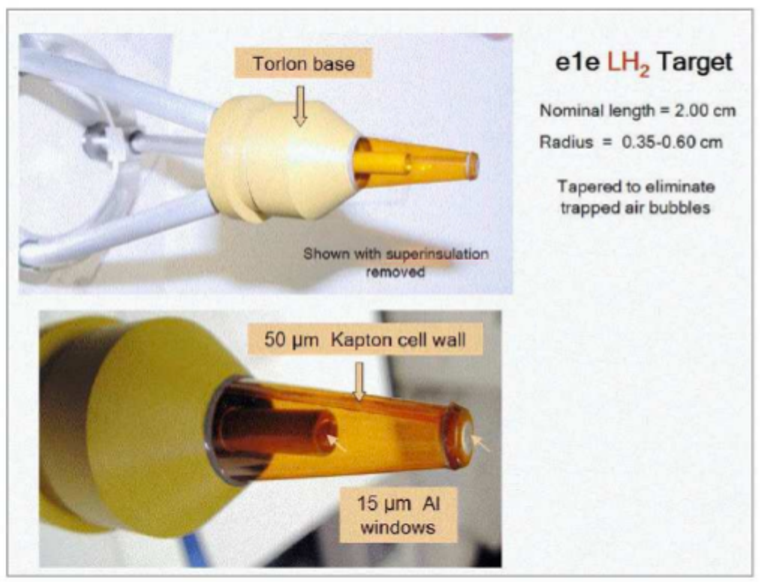
\includegraphics[width=5cm,keepaspectratio]{pictures/vertex/e1e_target_new.pdf}
\vspace{-0.1cm}
\caption{(colors online) The target cell and support structure used during ``e1e" run period.}
\label{fig:e1e_target}
\end{center}
\end{figure} 

Experimental configuration for the particular dataset was the following. The torus current was 2250~A and the mini torus current 5995~A.
The data  were obtained with the 2 cm long liquid hydrogen target located at -0.4 cm along z-axis and a 2.039 GeV polarized electron beam.


The target is specific to the ``e1e" experiment and its setup is presented in Fig.~\ref{fig:e1e_target}. It has a conical shape with the diameter varying from 0.4 to 0.6 cm. The reason for the target to be conical originates from the following issue. In some instances cooling system could not extract all the heat generated by the beam and the hydrogen in the target cell could boil. If bubbles stay along the beamline, the real luminosity would deviate from the expected value and the absolute measurement would lack accuracy. The conical shape helps to direct bubbles upwards and into a wider area of the target, thus clearing the beamline. The target cell has entry and exit 15-$\mu$m-thick aluminum windows. Beside this, an aluminum foil is located upstream at the distance two cm from the target center.  This foil is made exactly the same as the entry/exit windows of the target cell and can serve for both  the estimation of the number of events originated in the target windows and the precise determination of the target $z$ position along the beamline.




\begin{figure}[htp]
\begin{center}
 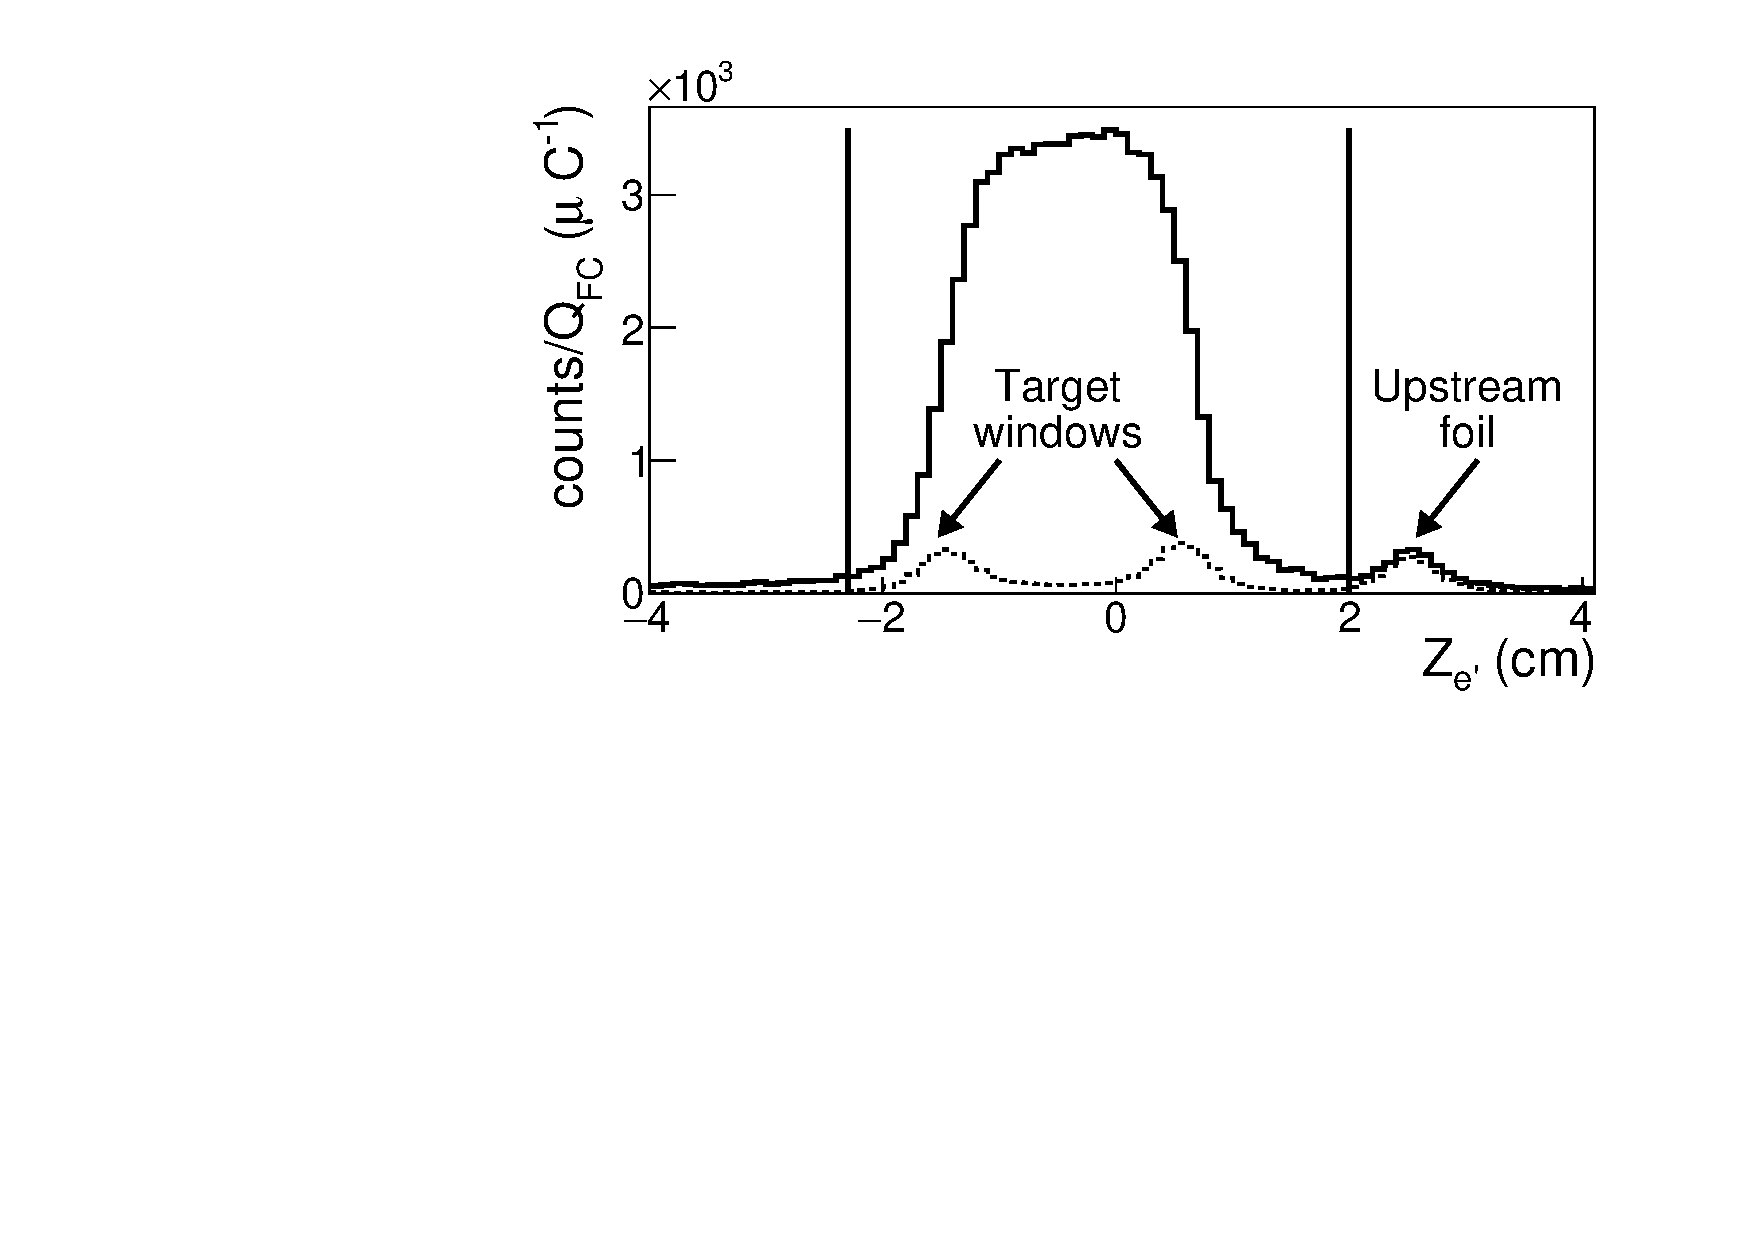
\includegraphics[width=8cm,keepaspectratio]{pictures/vertex/vertex_new.pdf}
\vspace{-0.1cm}
\caption{Distributions of the electron $z$ coordinate at the vertex for full (solid curve) and empty (dashed curve) target runs. Vertical lines show the applied cuts. Both full and empty target distributions are normalized to the corresponding charge accumulated on the Faraday Cup (FC).}
\label{fig:zvertex}
\end{center}
\end{figure} 

The dataset includes either runs with target cell filled out with liquide hydrogen (full target runs) as well as runs with empty target cell (empty target runs). The latter serve to subtract contribution from the non-signal events produced  by the scattering of electrons on the target windows. 
In Fig.~\ref{fig:zvertex} distributions of electron coordinate $z$ at the interaction vertex are shown for events from both empty (dashed curve) and full (solid curve) target runs. Both of them are normalized to the corresponded charge accumulated on the Faraday Cup (FC). The value of the vertex coordinate $z$ was corrected for the effects of beam-offset at the stage of data ``cooking". Both distributions in Fig.~\ref{fig:zvertex} demonstrate the well-separated peak around $z_{e'} = 2.4$~cm originated from the forward aluminum foil. The distribution of events from the empty target runs also shows two other similar peaks that correspond to the windows of the target cell. In addition to the empty target event subtraction the cut on $z$ coordinate of electron is applied. This cut is shown by two vertical lines in Fig.~\ref{fig:zvertex}, events outside these lines are excluded from the consideration. 
 
\section{Exclusive reaction event selection}
\label{expt}

To identify the reaction $e p \rightarrow e' p' \pi^{+} \pi^{-}$ the scattered electron and at least two final state hadrons need to be registered, while the four-momentum of the remaning hadron can be restored from the energy-momentum conservation.
The first in time particle that gives signals in all four parts of the CLAS detector (DC, CC, TOF, and EC) is chosen as electron candidate for each event. To identify hadrons only signals in DC and TOF are required.


\subsection{Electron identification}

To reveal good electrons from the electron candidates  electromagnetic calorimeter (EC) and \v Cerenkov counter (CC) responses need to be analyzed.

According to~\cite{Egian:007} overall EC resolution, as well as uncertainties in the EC output summing electronics lead to the fluctuation of the EC response near the hardware threshold. Therefore, to select only reliable EC signals the minimal cut on the scattered electron momentum $P_{e'}$ should be applied on the software level. As it is suggested in~\cite{Egian:007} this cut is chosen to be $P_{e'} > 0.461$~GeV.


Then so-called sampling fraction cut is applied to  eliminate in part pion contamination. To develop this cut the fact that electrons and pions
have different  energy deposition patterns in EC was used. An electron produces an electromagnetic shower, where the
deposited energy $(E_{tot})$ is proportional to its momentum $(P_{e'})$, while a $\pi^{-}$ as  a minimum ionizing particle loses a constant
amount of energy per scintillator (2~MeV/cm) independently of its momentum. 
Therefore, for electrons the quantity $E_{tot}/P_{e'}$ plotted as a function of $P_{e'}$ should follow the straight line that is parallel to the $X$-axis and located around the value 1/3 on the $Y$-axis, since electrons lose 2/3 of their energy in lead sheets (in reality this line has a slight slope).


In Fig.~\ref{fig:ec_cut} total energy deposited in EC sector one divided by the particle momentum is shown as function of particle momentum for data (top plot) and Monte Carlo (bottom plot). In this figure cut on minimal scattered electron momentum is shown by the vertical line, while two other curves correspond to the sampling fraction cut which was determined via Gaussian fit of different momentum slices of the distribution. The distributions for experimental data and Monte Carlo simulation differ, since the former was plotted for inclusive electrons while the latter for simulated double pion events only.
Mean value of the simulated distribution turned out to be slightly below than that of the experimental one 
due to the inaccuracy in reproduction of electromagnetic showers in the Monte Carlo reconstruction procedure.


\begin{figure}[htp]
\begin{center}
 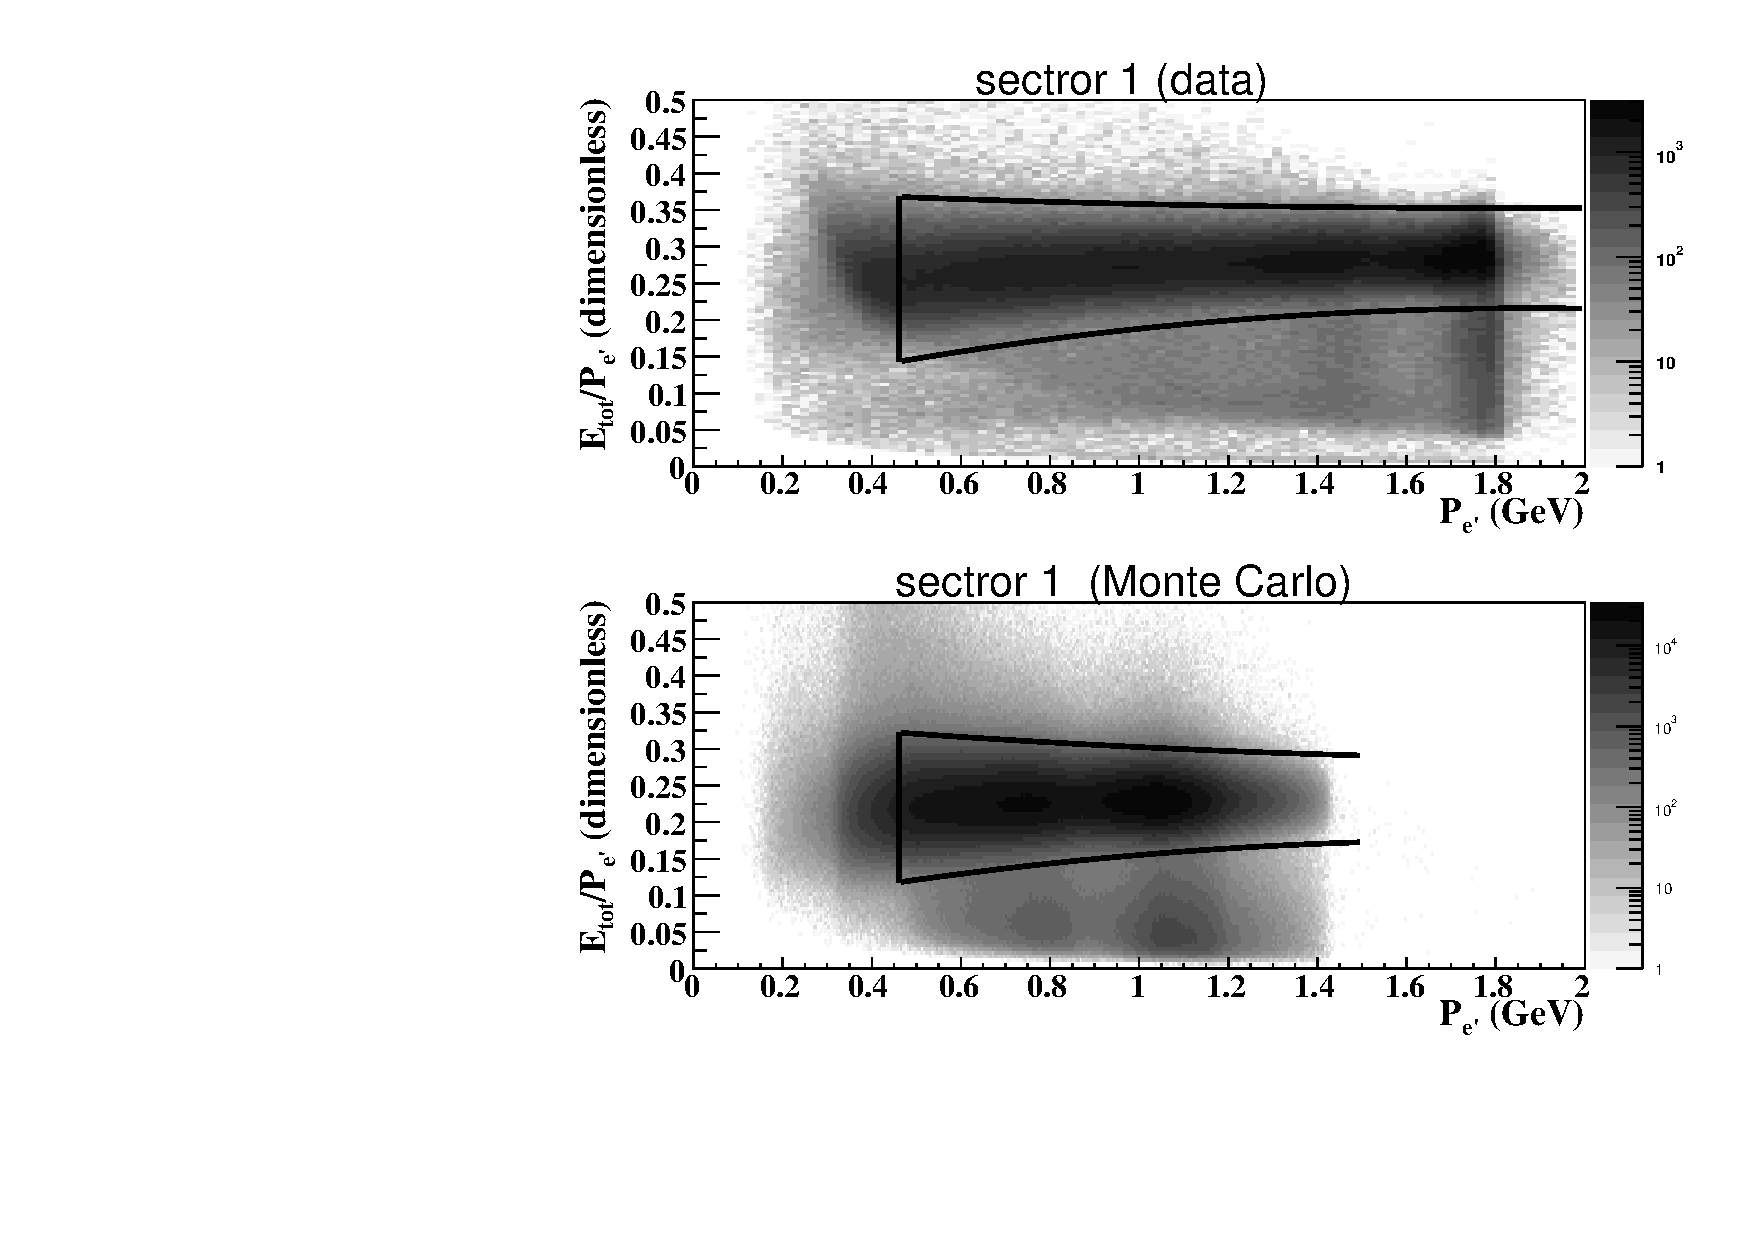
\includegraphics[width=7cm,keepaspectratio]{pictures/electron_id/ec_cut.pdf}
\vspace{-0.1cm}
\caption{Sampling fraction distributions for the data (top plot) and Monte Carlo (bottom plot). Both plots correspond to CLAS sector one. Events between the curves are treated as good electron candidates.}
\label{fig:ec_cut}
\end{center}
\end{figure} 


To improve the quality of electron candidate selection and $\pi^{-}/e^{-}$ separation a \v Cerenkov counter is used.
It turned out that CC had some inefficient zones  and their map could not be reproduced by Monte Carlo. Moreover, as it was shown in~\cite{Osipenko:2004} there was a contamination in the measured CC spectrum that manifested itself as a so-called single photoelectron peak, which was actually located at a few photoelectrons. The main source of this contamination was found to be the coincidence of accidental PMT noise signal with measured pion track~\cite{Osipenko:2004}. 

\begin{figure}[htp]
\begin{center}

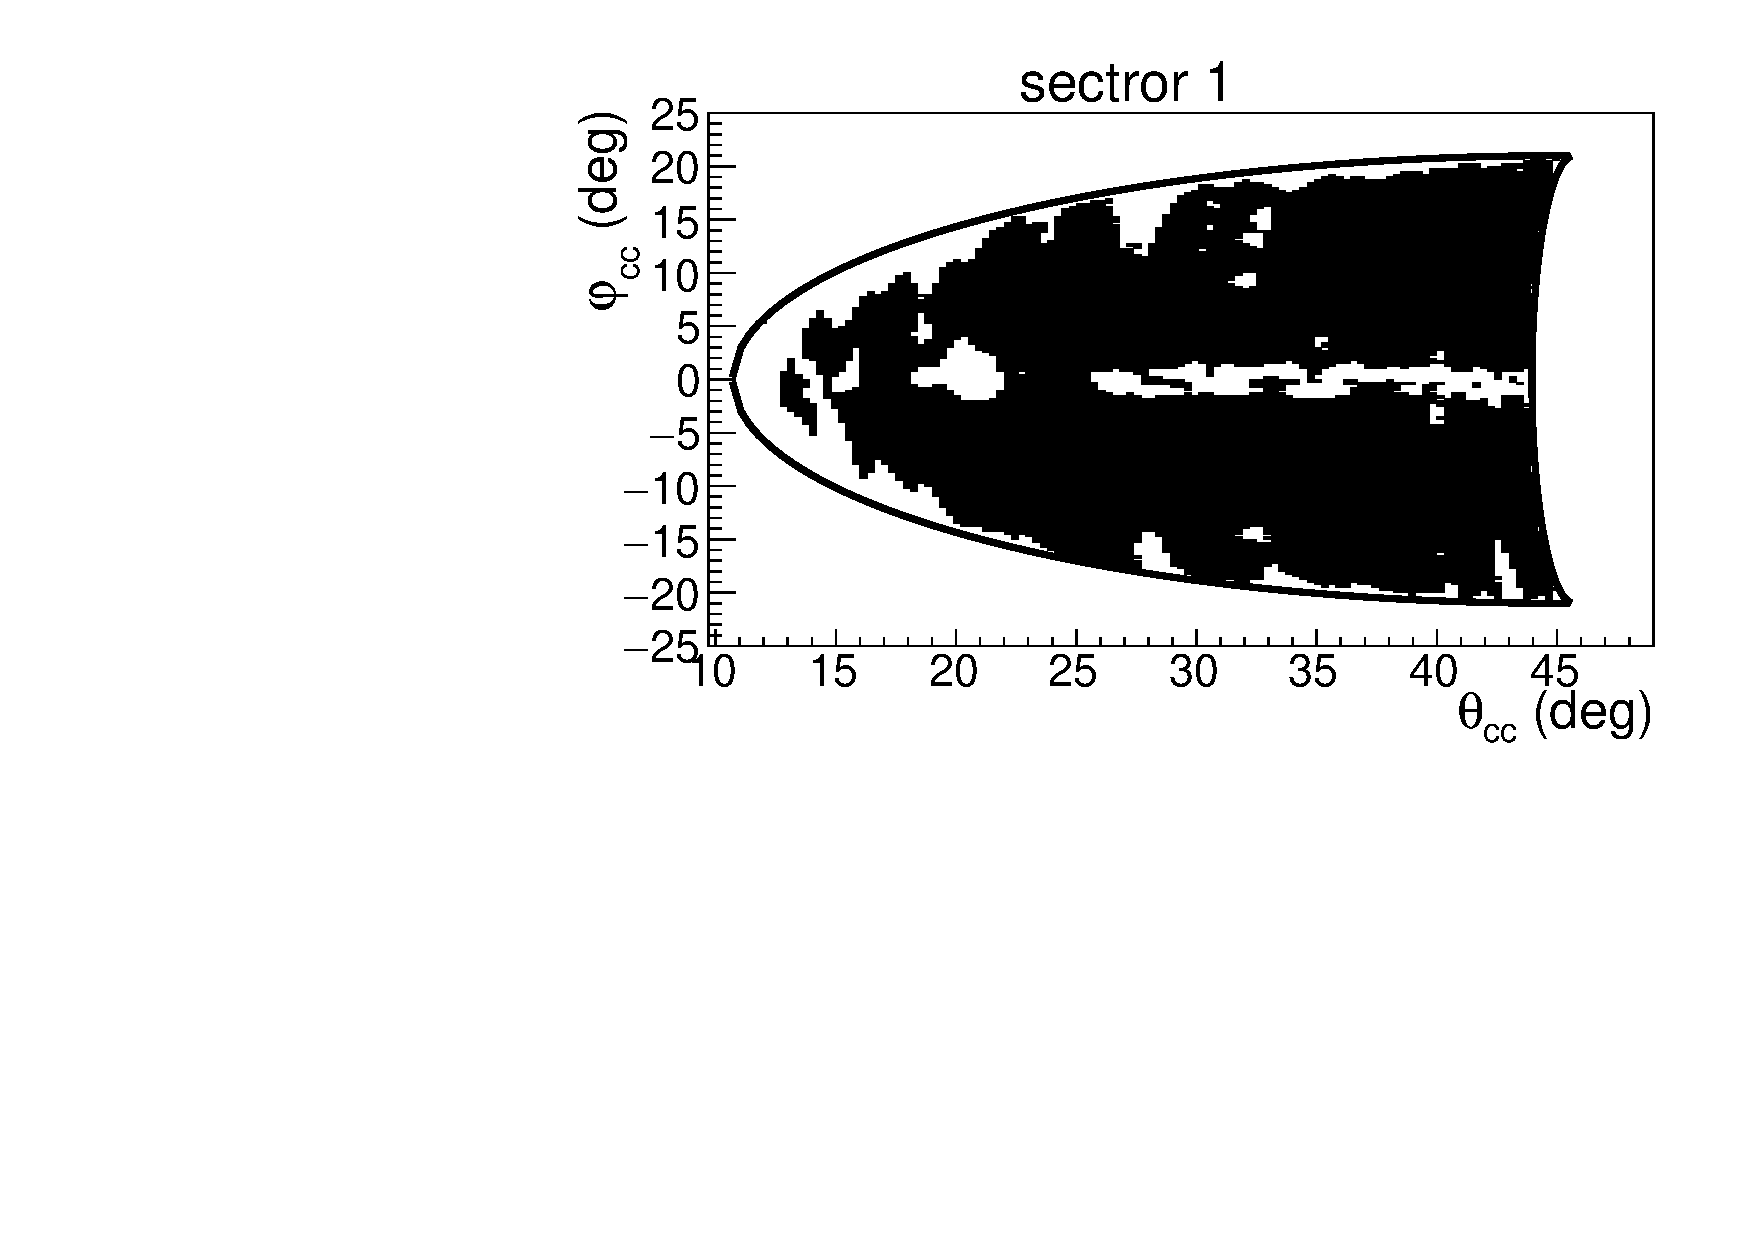
\includegraphics[width=7cm,keepaspectratio]{pictures/electron_id/ph_vs_ph_cc.pdf}
\vspace{-0.1cm}
\caption{Zones where CC is efficient enough to accept good electron candidates are shown in black as function of the polar ($\theta_{cc}$) and azimuthal ($\varphi_{cc}$) angles in the CC plane for CLAS sector one. }
\label{fig:ph_vs_ph_cc}
\end{center}
\end{figure} 

Signals from inefficient zones being depleted of good events have therefore strong relative noise contribution that in turns results in very pronounced single photoelectron peak. This fact was used for geometrical separation of CC regions with reliable detection efficiency from the inefficient areas.  In Fig.~\ref{fig:ph_vs_ph_cc} the distribution of zones with small relative noise contribution are shown in black as a function of polar and azimutal angles defined in the CC plane for CLAS sector one. As it is seen in Fig.~\ref{fig:ph_vs_ph_cc}, there is an inefficient area in the middle of the sector shown in white, that is expected since two CC mirrors are joined there. The curves which are superimosed on the distribution  show fiducial cut that is applied in the CC plane. For both experimental data and Monte Carlo simulation only electron candidates originated from black regions within the fiducial cut were analyized.



\begin{figure}[htp]
\begin{center}
 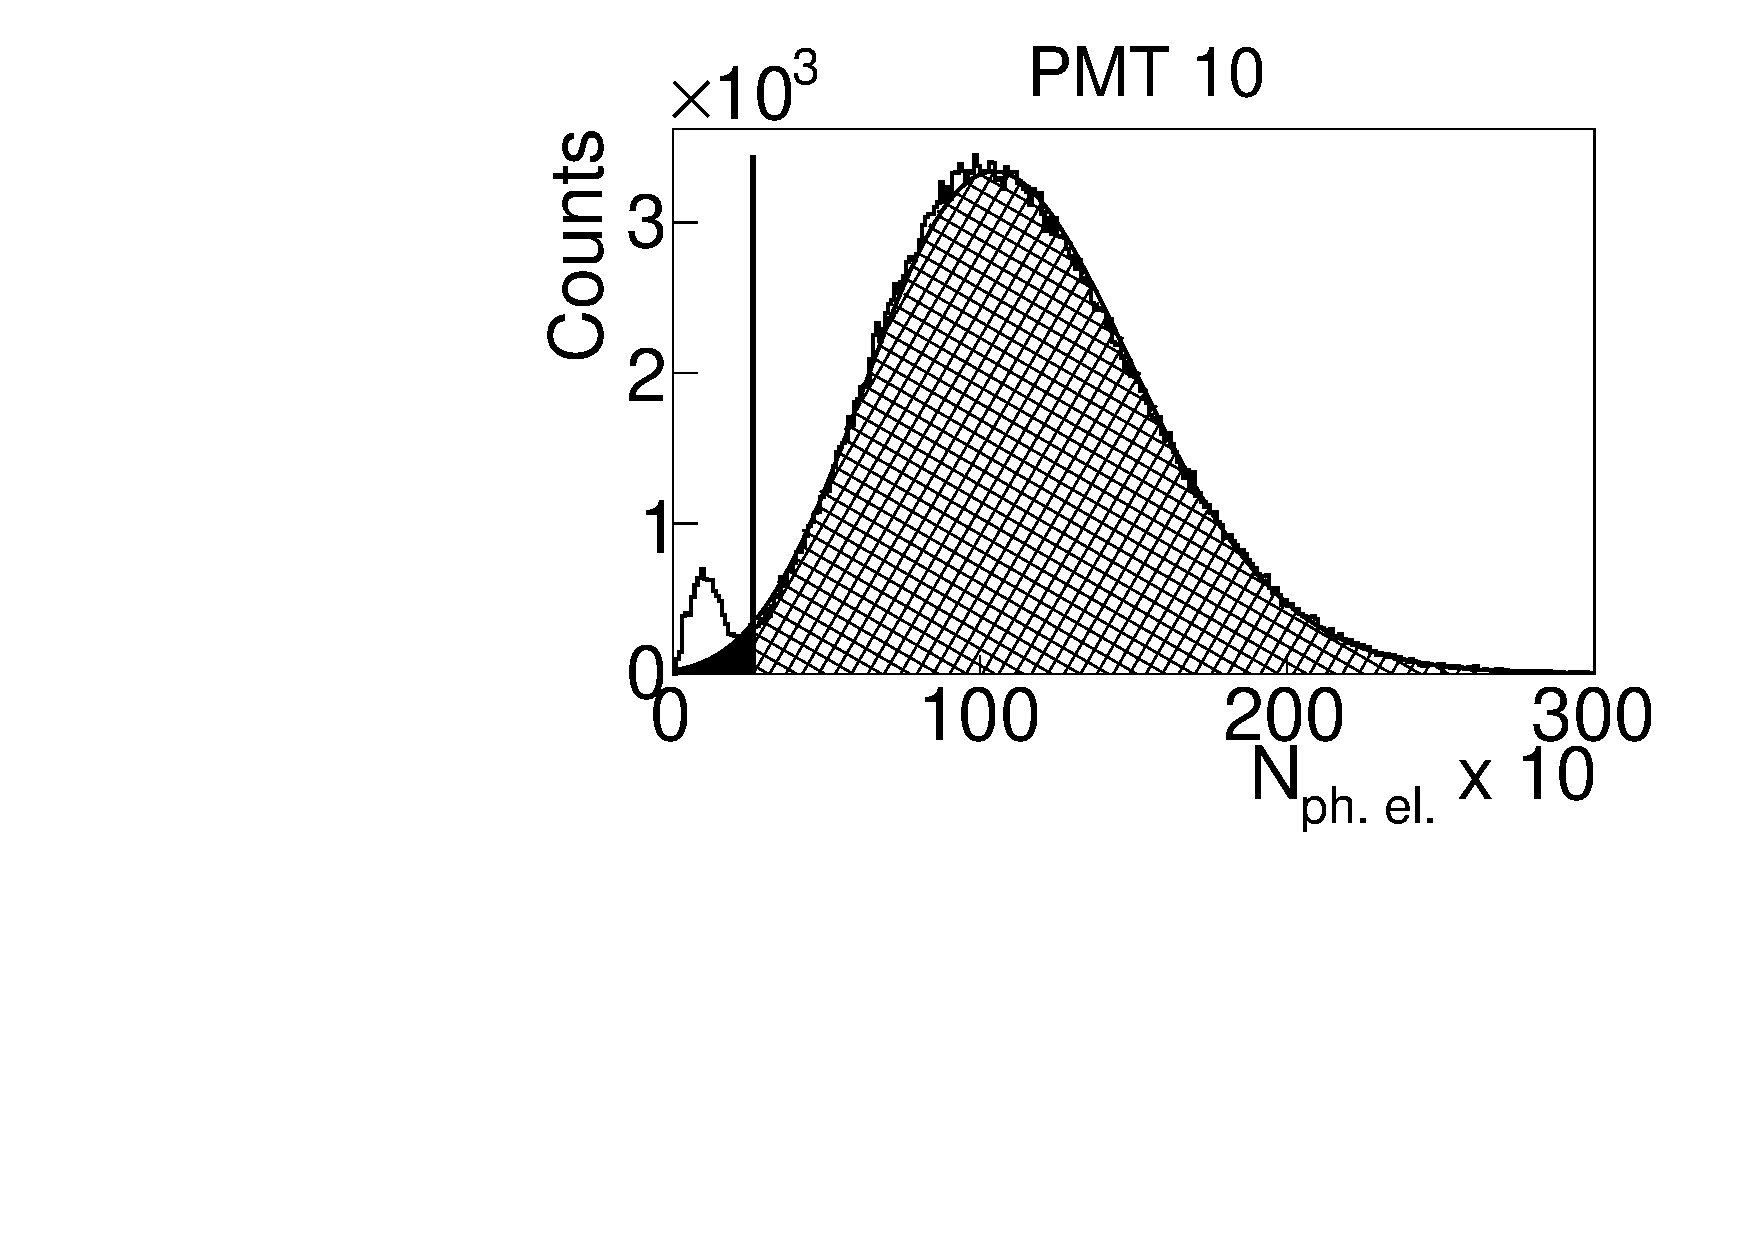
\includegraphics[width=7cm,keepaspectratio]{pictures/electron_id/ph_el.pdf}
\vspace{-0.1cm}
\caption{Number of photoelectrons multiplied by ten for the left side PMT in segment ten of sector one of CC. Black curve shows the fit by function~\eqref{eq:cc_Poisson}. Vertical line shows the applied cut. Regions that are needed to calculate the correction factor are shown in hatch and black. }
\label{fig:ph_el}
\end{center}
\end{figure} 
 

 



Although being substentionally reduced after eliminating of signals from inefficient zones, single photoelectron peak is still presented in the experimental CC spectrum as it is shown in Fig.~\ref{fig:ph_el} for left PMT in CC segment ten from sector one. This peak in photoelectron distribution is cut out for each PMT in each CC segment individually. The cut position is shown by the vertical line in Fig.~\ref{fig:ph_el}.
Since Monte Carlo does not reproduce photoelectron spectrum well enough, this cut is applied only to the experimental data, and good electrons lost in this way are recovered by the following procedure. The part of the distribution on the right side of the vertical line is fit by the function $y = y(x)$, which is a slightly modified Poisson distribution~\eqref{eq:cc_Poisson}. 

\begin{equation}
y = P_{1}\left(\frac{P_{3}^{\frac{x}{P_{2}}}}{\Gamma\left(\frac{x}{P_{2}}+1\right)}
\right)e^{-P_{3}},
\label{eq:cc_Poisson}
\end{equation}

where $P_{1}$, $P_{2}$, and $P_{3}$ are free fit parameters.

The fitting function is then continued into the region on the left side of the vertical line. In this way the two regions, shown in black and hatch in Fig.~\ref{fig:ph_el}, are determined. Finally, the correction factors are defined by~\eqref{eq:cc_corr_fact} and applied as a weight for each event which corresponds to the particular PMT. 

\begin{equation}
F_{ph.\,\, el.} = \frac{{hatched\,\,  area} {\,\,+\,\,} {black\,\,  area}}{{hatched\,\,  area}}
\label{eq:cc_corr_fact}
\end{equation}

The correction factor $F_{ph.\,\, el.}$ depends on PMT number and is typically on a level of a few percent.







 






%%%%%%%%%%%%%%%%%%%%%%%%%%%%%%%%%%%%%%%%%%%%%%%%%%%%%%%%%%%%%%%%%%%%%%%%%%%%%%%%%%%%%%%%%%%%%%%%%%%%%%%%%%

\subsection{Hadron identification}

\begin{figure}[htp]
\begin{center}
 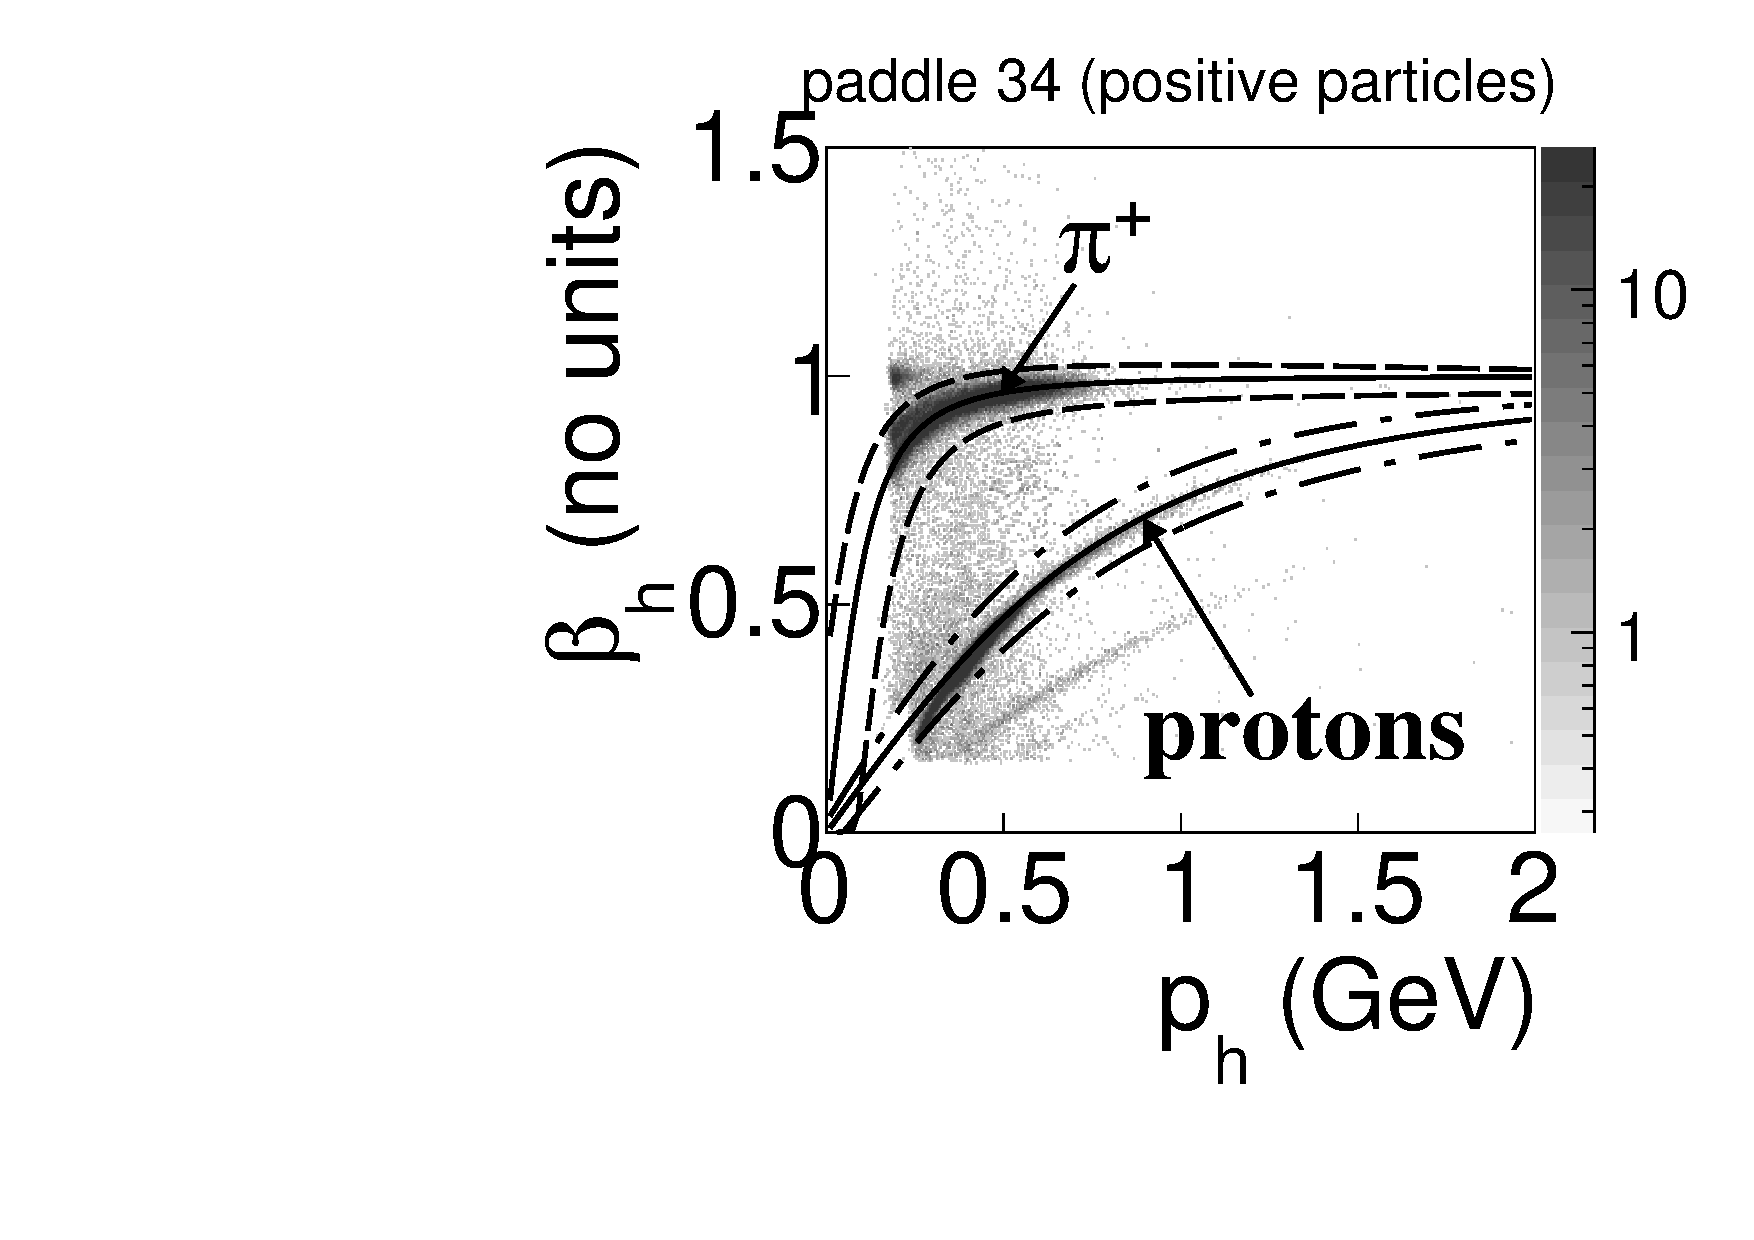
\includegraphics[width=6cm,keepaspectratio]{pictures/hadron_id/b_vs_p_positiv_time_corr.pdf}
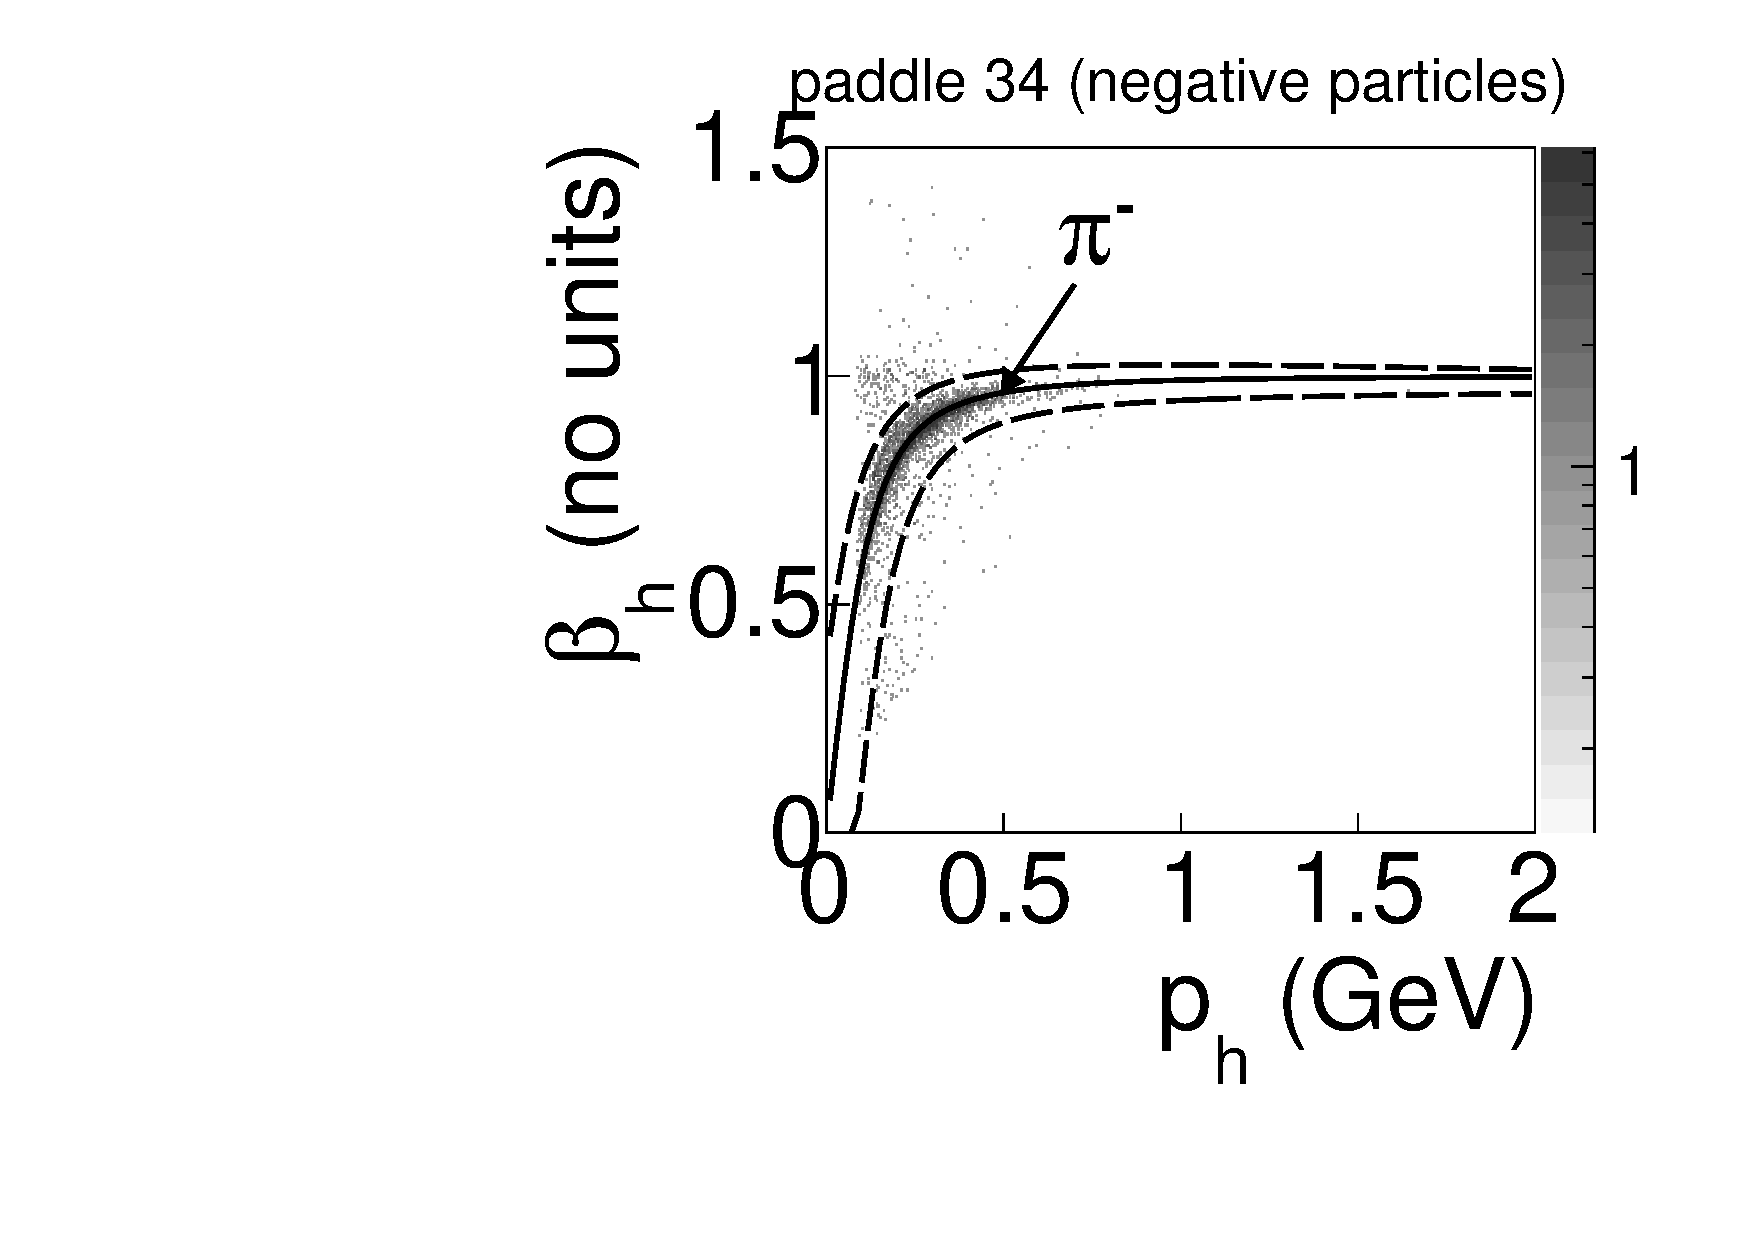
\includegraphics[width=6cm,keepaspectratio]{pictures/hadron_id/b_vs_p_negative_time_corr.pdf} 
\vspace{-0.1cm}
\caption{$\beta_{h}$ versus momentum distributions for positively charged hadron candidates (top plot) and  negatively charged hadron candidates (bottom plot) for scintillator number 34 in CLAS sector one. Black solid curves correspond to the nominal $\beta_{n}$ given by~\eqref{eq:hadron_hadronmass}. 
Events between the dashed and dot-dashed curves are selected as $\pi^{+}$ ($\pi^{-}$) and protons, respectively.}
\label{fig:b_vs_p}
\end{center}
\end{figure} 



The CLAS TOF system provides information, based on which the 
velocity $(\beta_{h} = v_{h}/c)$ of the hadron candidate can be determined.  
The value of the hadron candidate momentum $(p_{h})$
is in turn provided by the Drift
Chambers.  The
charged hadron can be identified by the comparison of $\beta_{h}$ determined by TOF with $\beta_{n}$ given by the following formula~\eqref{eq:hadron_hadronmass}.
\begin{equation}
\beta_{n}=\frac{p_{h}}{\sqrt{p_{h}^{2}+m_{h}^{2}}}.
\label{eq:hadron_hadronmass}
\end{equation}
In~\eqref{eq:hadron_hadronmass} $\beta_{n}$ is a so-called nominal value that is calculated using the hadron candidate momentum $(p_{h})$ and exact hadron mass assumption $m_{h}$. 






The experimental event distributions $\beta_{h}$ versus $p_{h}$ were investigated for each TOF paddle in each CLAS sector. An example of these distributions is shown in Fig.~\ref{fig:b_vs_p} for positively charged hadron candidates (top plot) and negatively charged hadron candidates (bottom plot). 
 The example is given for the paddle 34 of the CLAS sector one. In Fig.~\ref{fig:b_vs_p} solid curves are given for $\beta_{n}$ calculated according to~\eqref{eq:hadron_hadronmass} for the corresponded hadron mass assumptions. 
The event bands of the pion and proton candidates are clearly seen around the corresponded $\beta_{n}$ curves.  
The dashed curves show the cuts that were used for pions identification, while the dot-dashed curves serve to identify protons. 

It was figured out that during the run some TOF paddles worked improperly and therefore their signals were considered to be unreliable and were removed from the consideration either for data and simulation. 
For all remaining properly worked paddles the hadron identification cuts were chosen to be the same as shown in Fig.~\ref{fig:b_vs_p}. They were applied for both experimental and reconstructed Monte Carlo events. It needs to be mentioned that in experimental distributions hadron candidate bands were slightly shifted from the nominal positions for some paddles. To cure that effect a special procedure of correcting the timing information provided by TOF was used.




\subsection{Momentum correction}

Due to the slight misalignments in the DC position,  small inaccuracies in
the description of the torus magnetic field, and other possible reasons the momentum and angle of
particles may have some small systematic deviations from the real values. 
Since the effects are of unknown origin, they cannot be simulated, and therefore a special  momentum correction procedure is needed for the experimental data. 
According to~\cite{KPark:momcorr} the evidence of the need of such corrections is most directly seen in the dependence of the elastic peak position on the azimutal angle of the scattered electron. It is shown in~\cite{KPark:momcorr} that the elastic peak position turned out to be shifted from the proton mass value and this shift depends on CLAS sector. 

The significance of the named above effect depends on beam energy. It was found that in this dataset with the beam energy 2.039 GeV  the small shift ($\sim$ 3 MeV) in elastic peak position took place, while the study~\cite{KPark:momcorr} demonstrated that in case of  5.754 GeV beam energy this shift reached 20 MeV. Moreover, the study~\cite{KPark:momcorr} also showed that this effect became discernible only if the particle momentum was sufficiently high (e.g. for pions the correction was needed only if their momentum was higher than 2 GeV). Thus, the small beam energy and the fact that in double pion kinematics hadrons carry only a small portion of the total momentum allow to come to the conclusion that for the presented data the correction is needed only for electrons, while deviation in hadron momenta can be neglected.

The electron momentum corrections used in this analysis had been developed according to~\cite{KPark:momcorr} for each CLAS sector individually and included  electron momentum magnitude correction as well as electron polar angle correction. Although the corrections had been established using elastic events, they were applied for all electron candidates in the dataset.  The influence of these corrections on the elastic peak position is shown in Fig.~\ref{fig:elast_pic_position}. As it is seen from Fig.~\ref{fig:elast_pic_position} the corrections bring the position of the elastic peak closer to the proton mass for all six CLAS sectors.


\begin{figure}[htp]
\begin{center}
 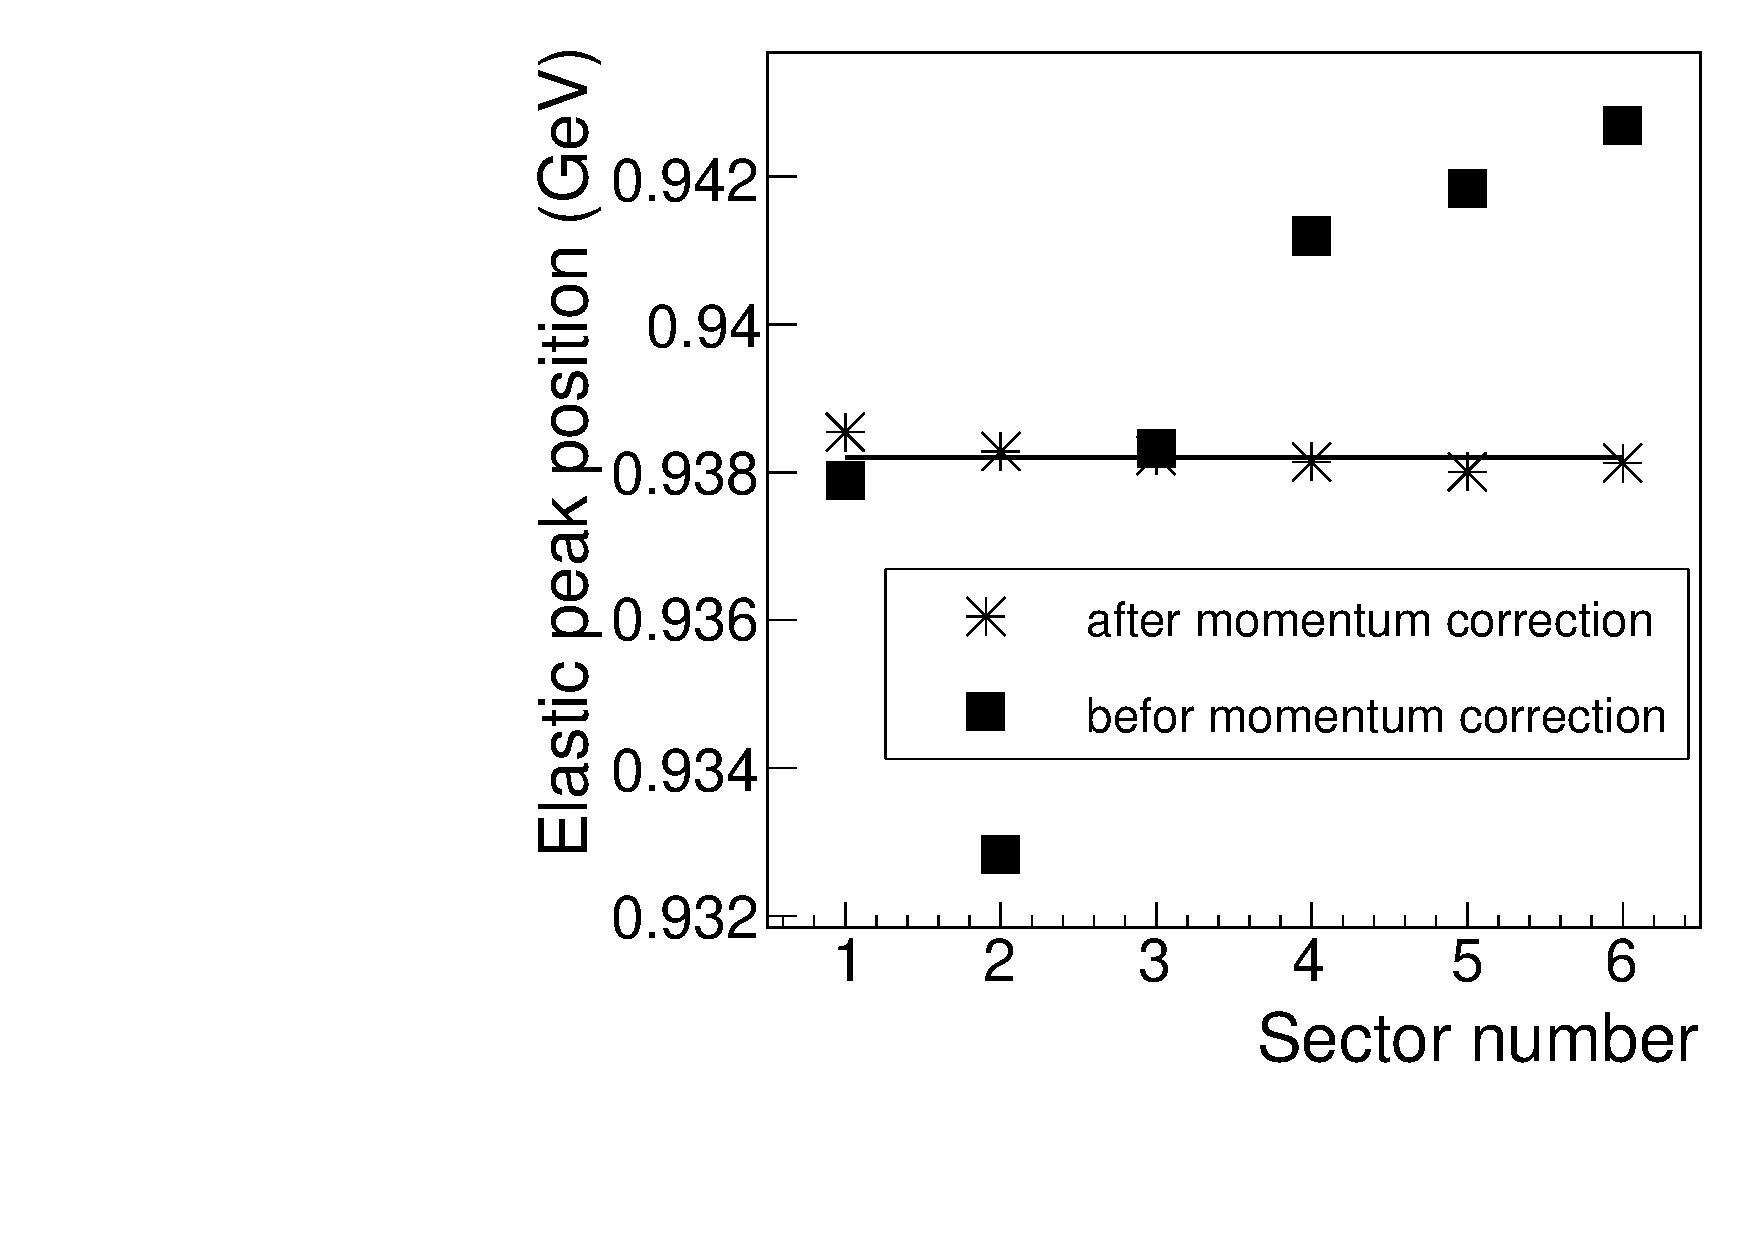
\includegraphics[width=6cm,keepaspectratio]{pictures/mom_corr/elast_pic_position.pdf}
\vspace{-0.1cm}
\caption{Elastic peak position for six CLAS sectors before (squares) and after (stars) electron momentum correction. Horizontal line shows the proton mass. }
\label{fig:elast_pic_position}
\end{center}
\end{figure} 

Although the named above effects do not lead to the substential distortions of the hadron momenta, hadrons lose part of their energy due to the interaction with detector and target media, hence their measured momentum appears to be lower than the ones the hadrons actually had right after the interaction. 
Simulation of the CLAS detector  correctly propagates hadrons through the media and therefore the effect of the hadron energy loss being included into the efficiency do not impact the extracted cross section value.
However in order to avoid shifts in distributions of some kinematical quantities (e.g. missing masses) from their expected values 
the energy loss correction was applied to the proton momentum magnitude (both experimental and reconstructed Monte Carlo),
 since the low-energetic protons are mostly affected by this effect.

\subsection{Other cuts}

\subsubsection{Fiducial cuts}

An active detection solid angle of the CLAS detector
 was smaller than $4\pi$~\cite{Me03}.
This happened because the areas covered by the torus field coils
 were not 
equipped with any detection system thus forming gaps in the azimutal angle coverage. In addition to that the detection area was also limited in polar angle from 8$^{o}$ up to 45$^{o}$ for electrons and up to 140$^{o}$ for other charged particles.
Moreover, the edges of the detection area do not provide a safe region
for particle registration, being affected by rescattering from the
coils, field distortions, and similar effects. Therefore it is now
a common practice to consider only those particles that were registered in ``safe" areas inside specific fiducial cuts, i.e. cuts on the kinematic variables
(momentum and angles) of each particle. These cuts are applied for both real events and Monte Carlo reconstructed events.

\begin{figure}[htp]
\begin{center}
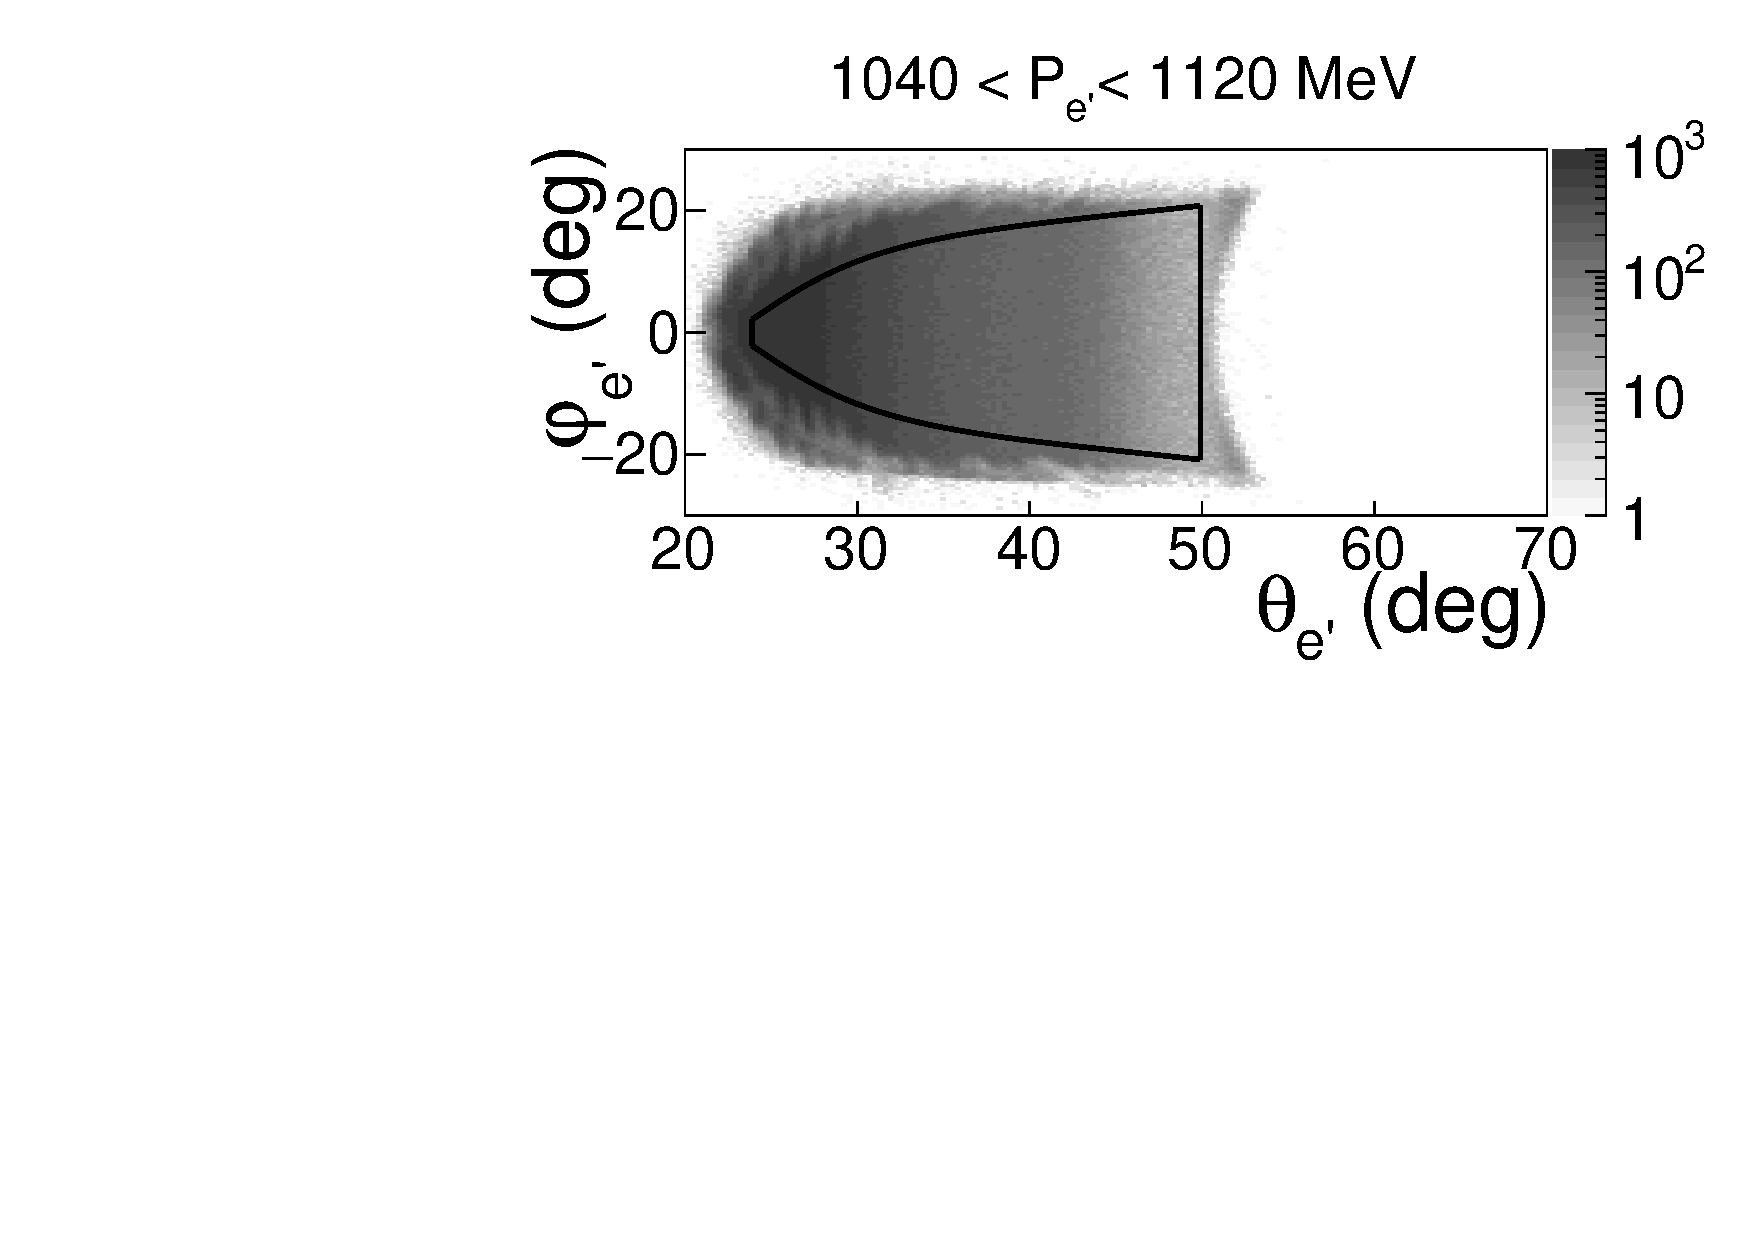
\includegraphics[width=7cm,keepaspectratio]{pictures/fiducial_cuts/electrons.pdf}
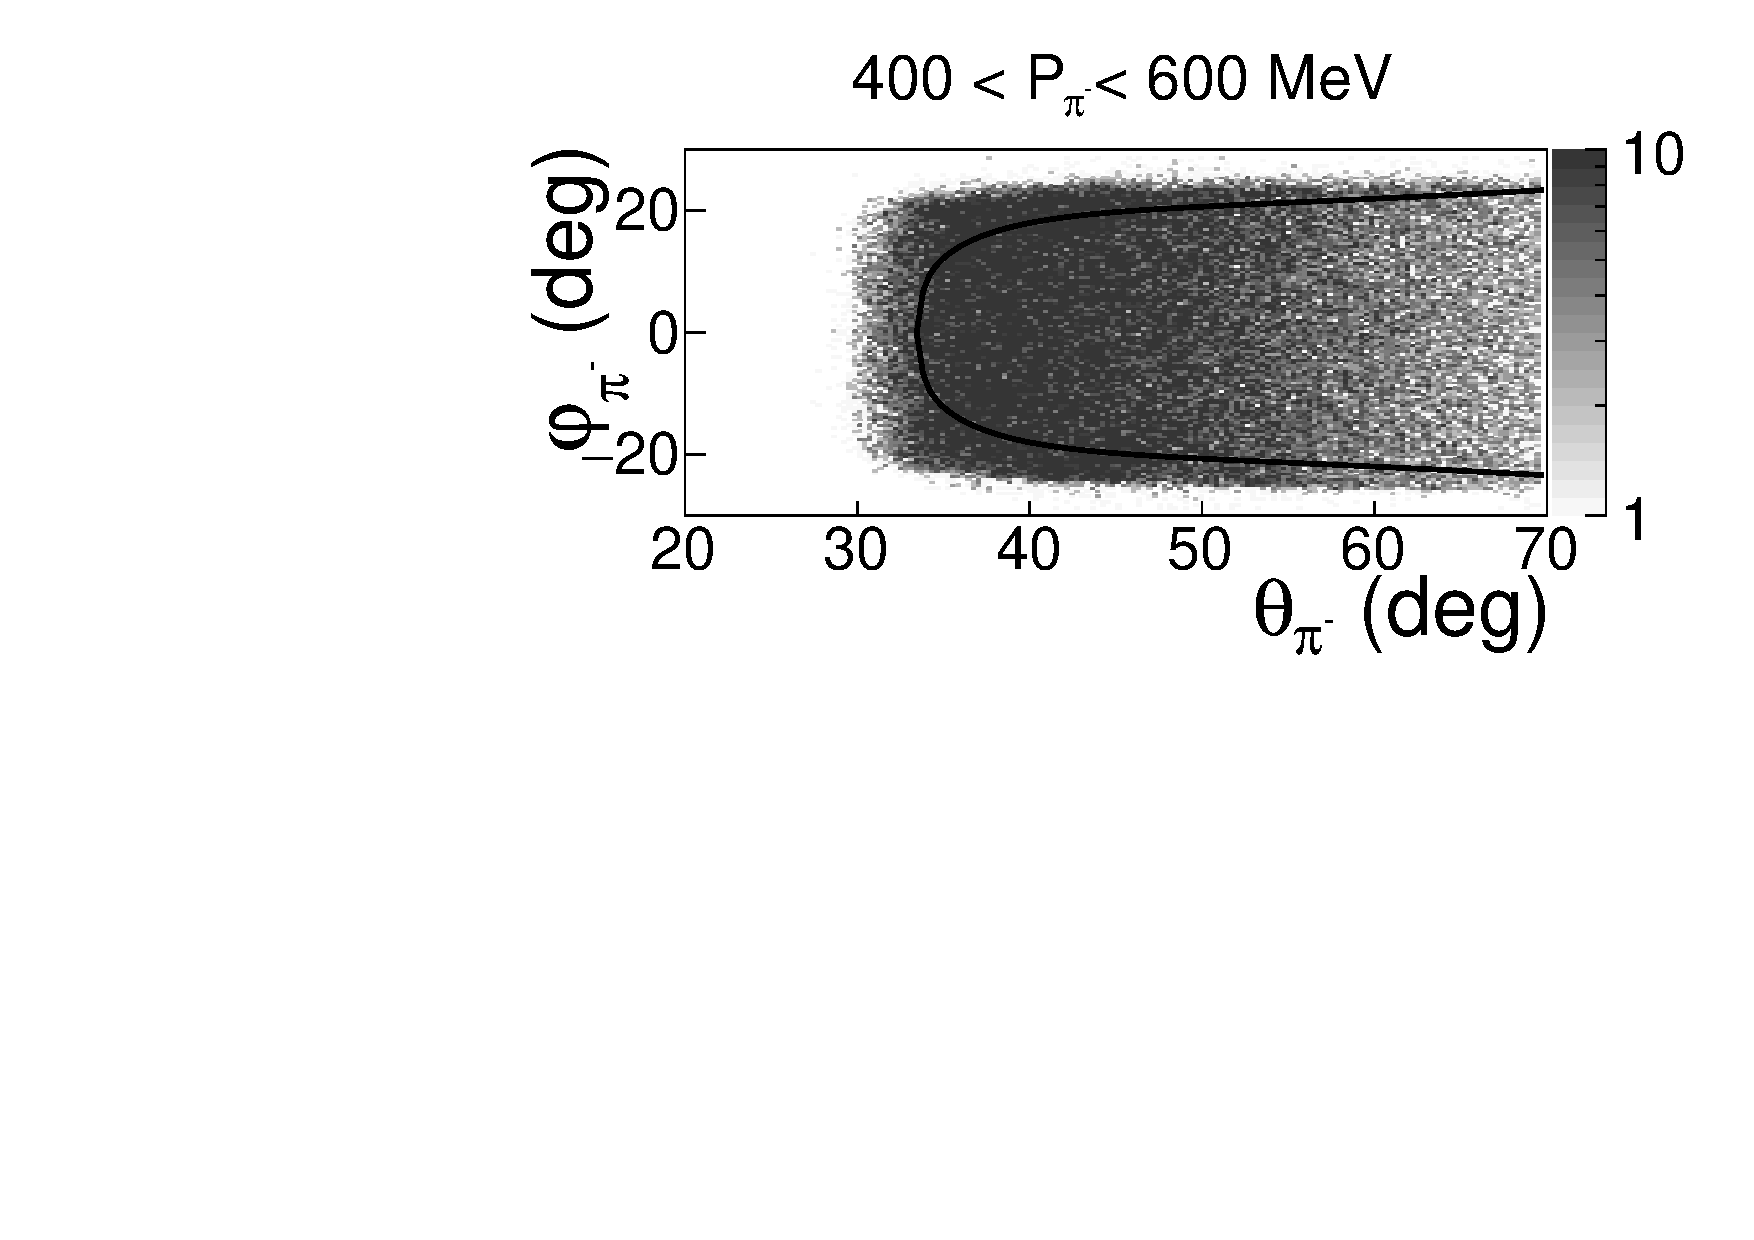
\includegraphics[width=7cm,keepaspectratio]{pictures/fiducial_cuts/pim.pdf} 
\vspace{-0.1cm}
\caption{Fiducial cuts for negatively charged particles. Top plot shows $\varphi$ versus $\theta$ destribution for electrons, while bottom plot corresponds to that for $\pi^{-}$. Both distributions are given for CLAS sector one and corresponding range over momentum specified in the plots.  Solid black curves stand for the applied fiducial cuts. }
\label{fig:fid_cuts_neg}
\end{center}
\end{figure} 

The ``e1e" run period had  the normal direction of the torus magnetic field that forces negatively charged particles to be inbending. For that type of particles sector independent, symmetrical, and momentum dependent cuts are applied. 
Fig.~\ref{fig:fid_cuts_neg} shows the number of registered electrons (top plot) and $\pi^{-}$ (bottom plot) as a function of angles $\varphi$ and $\theta$  for CLAS sector one and one slice over corresponded particle momentum. The angles $\varphi$ and $\theta$ are taken at the interaction vertex. Solid black curves correspond to the applied fiducial cuts. These cuts isolate the regions with relatively stable yield of events along azimutal angle. 


\begin{figure}[htp]
\begin{center}
 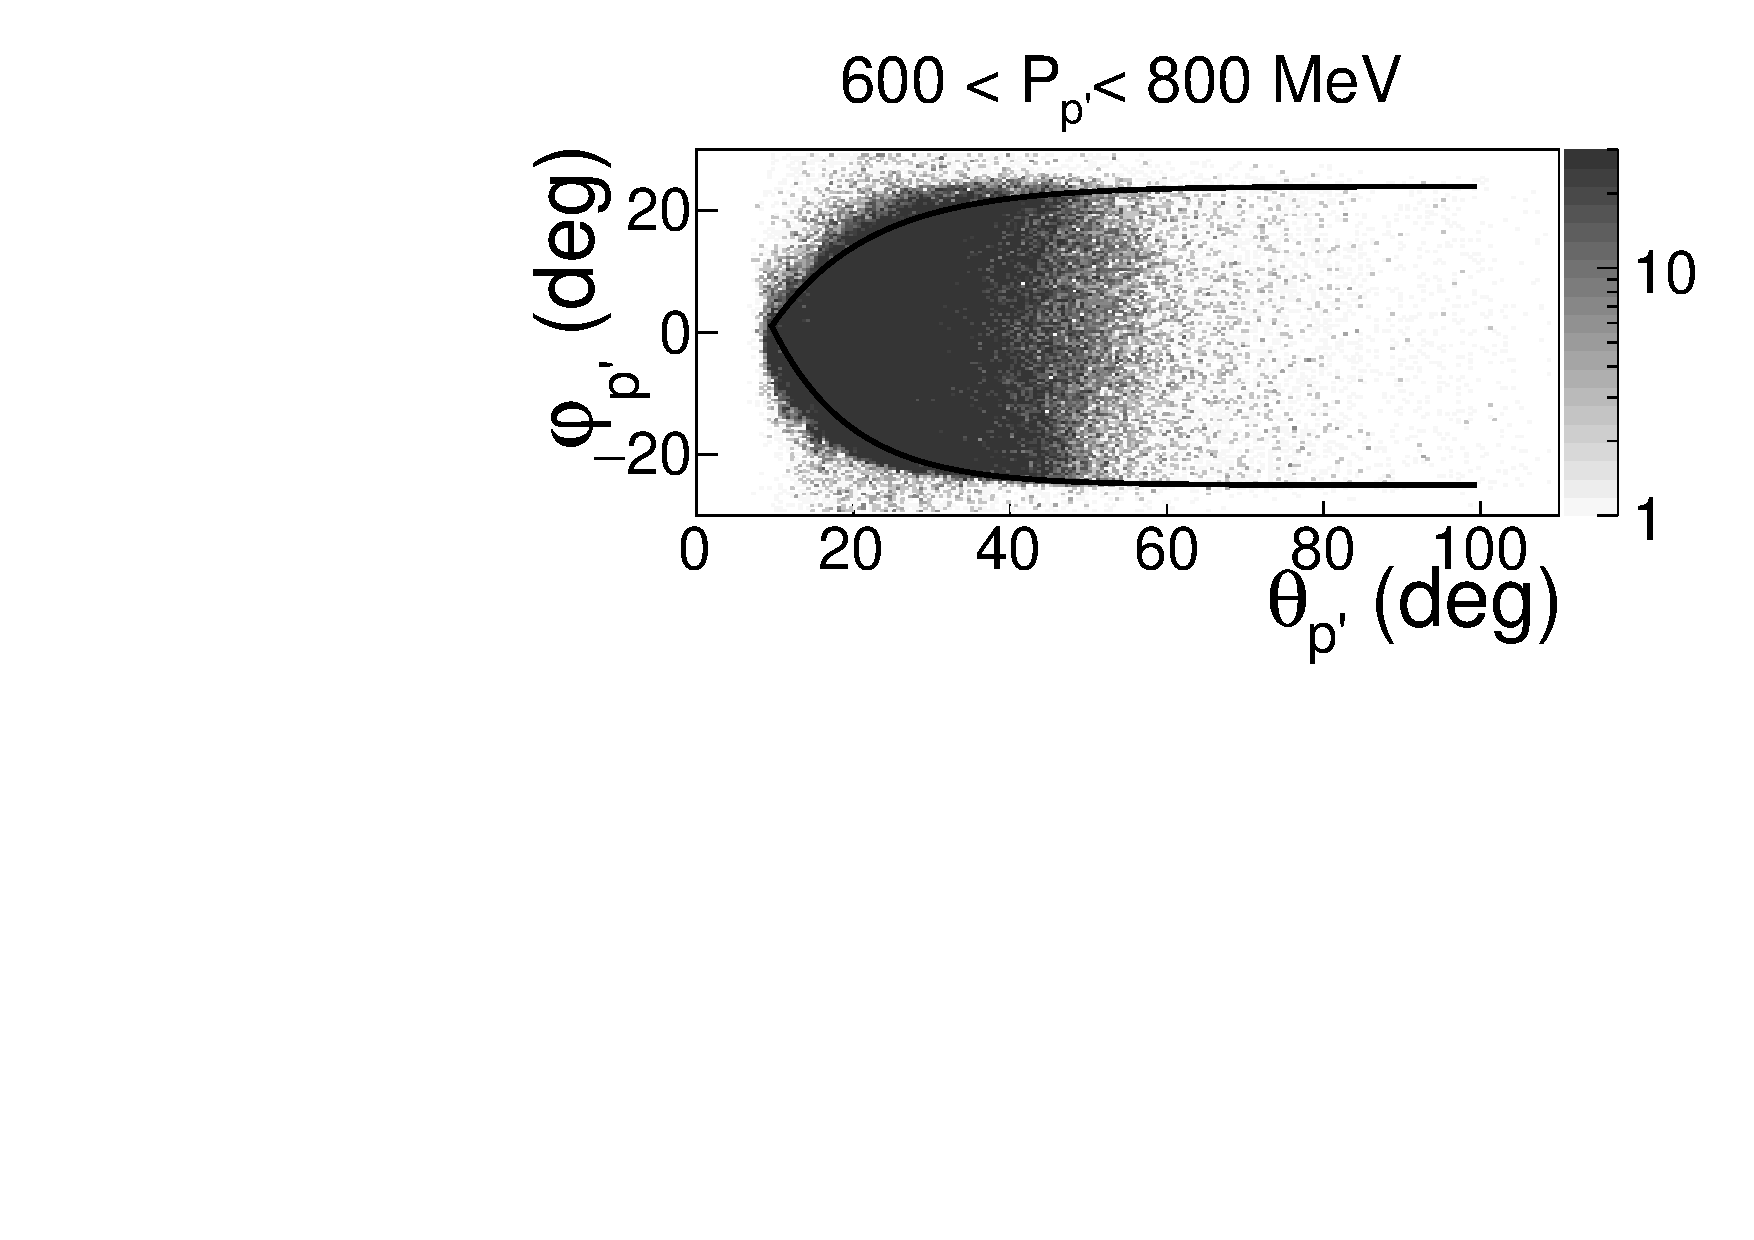
\includegraphics[width=7cm,keepaspectratio]{pictures/fiducial_cuts/protons.pdf}
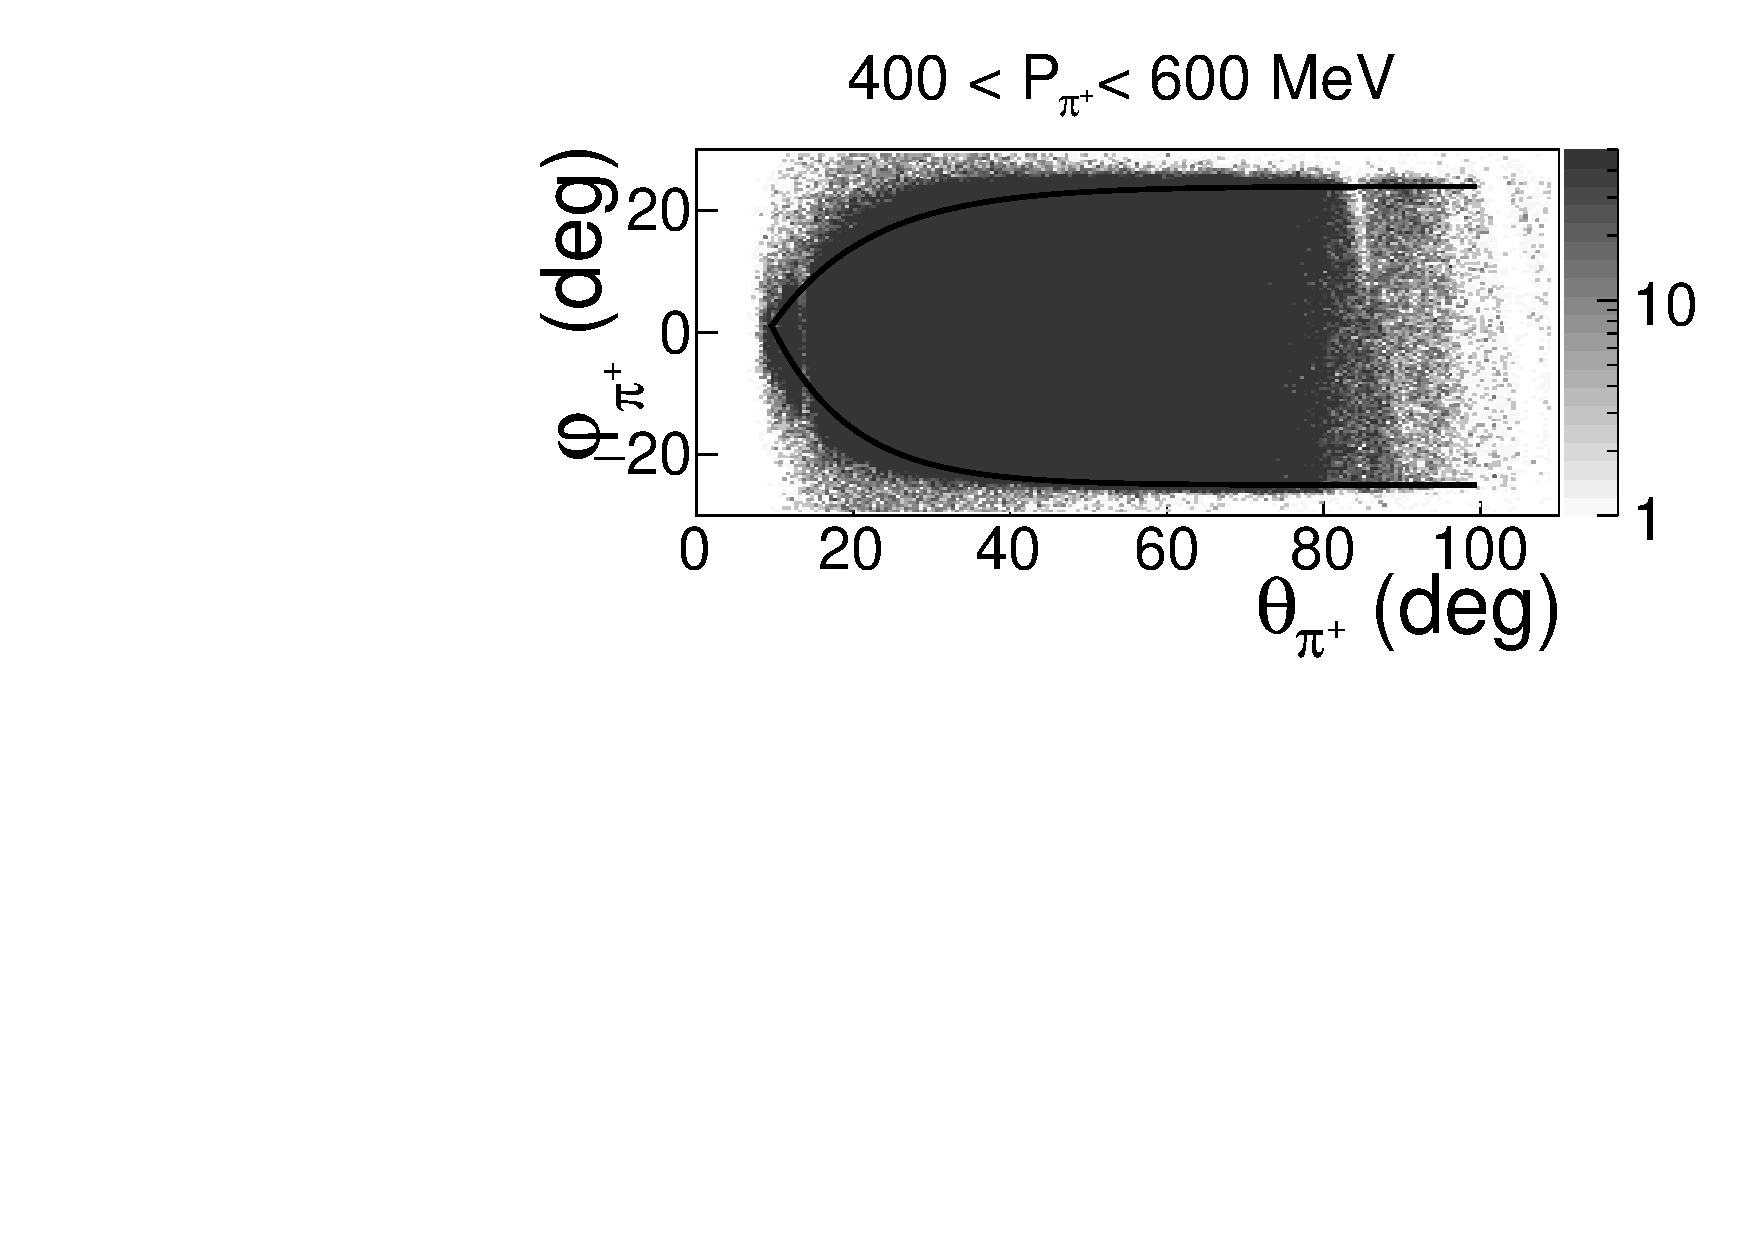
\includegraphics[width=7cm,keepaspectratio]{pictures/fiducial_cuts/pip.pdf} 
\vspace{-0.1cm}
\caption{Fiducial cuts for positively charged particles. Top plot shows $\varphi$ versus $\theta$ destribution for protons, while bottom plot corresponds to that for $\pi^{+}$. Both distributions are given for CLAS sector one and corresponding range over momentum specified in the plots.  Solid black curves stand for the applied fiducial cuts. }
\label{fig:fid_cuts_pos}
\end{center}
\end{figure} 



For positively charged particles, which were outbending in ``e1e" run period, momentum independent and slightly asymmetrical fiducial cuts are the best choice. These cuts were established in the same way as for negatively charged particles, i.e.
by selecting the areas with relatively stable event yield along the $\varphi$ angle. In Fig.~\ref{fig:fid_cuts_pos} these cuts shown by black curves are superimposed on $\varphi$ versus $\theta$ event distributions for protons (top plot) and $\pi^{+}$ (bottom plot). All angles are given at the interaction vertex.  


\begin{figure}[htp]
\begin{center}
 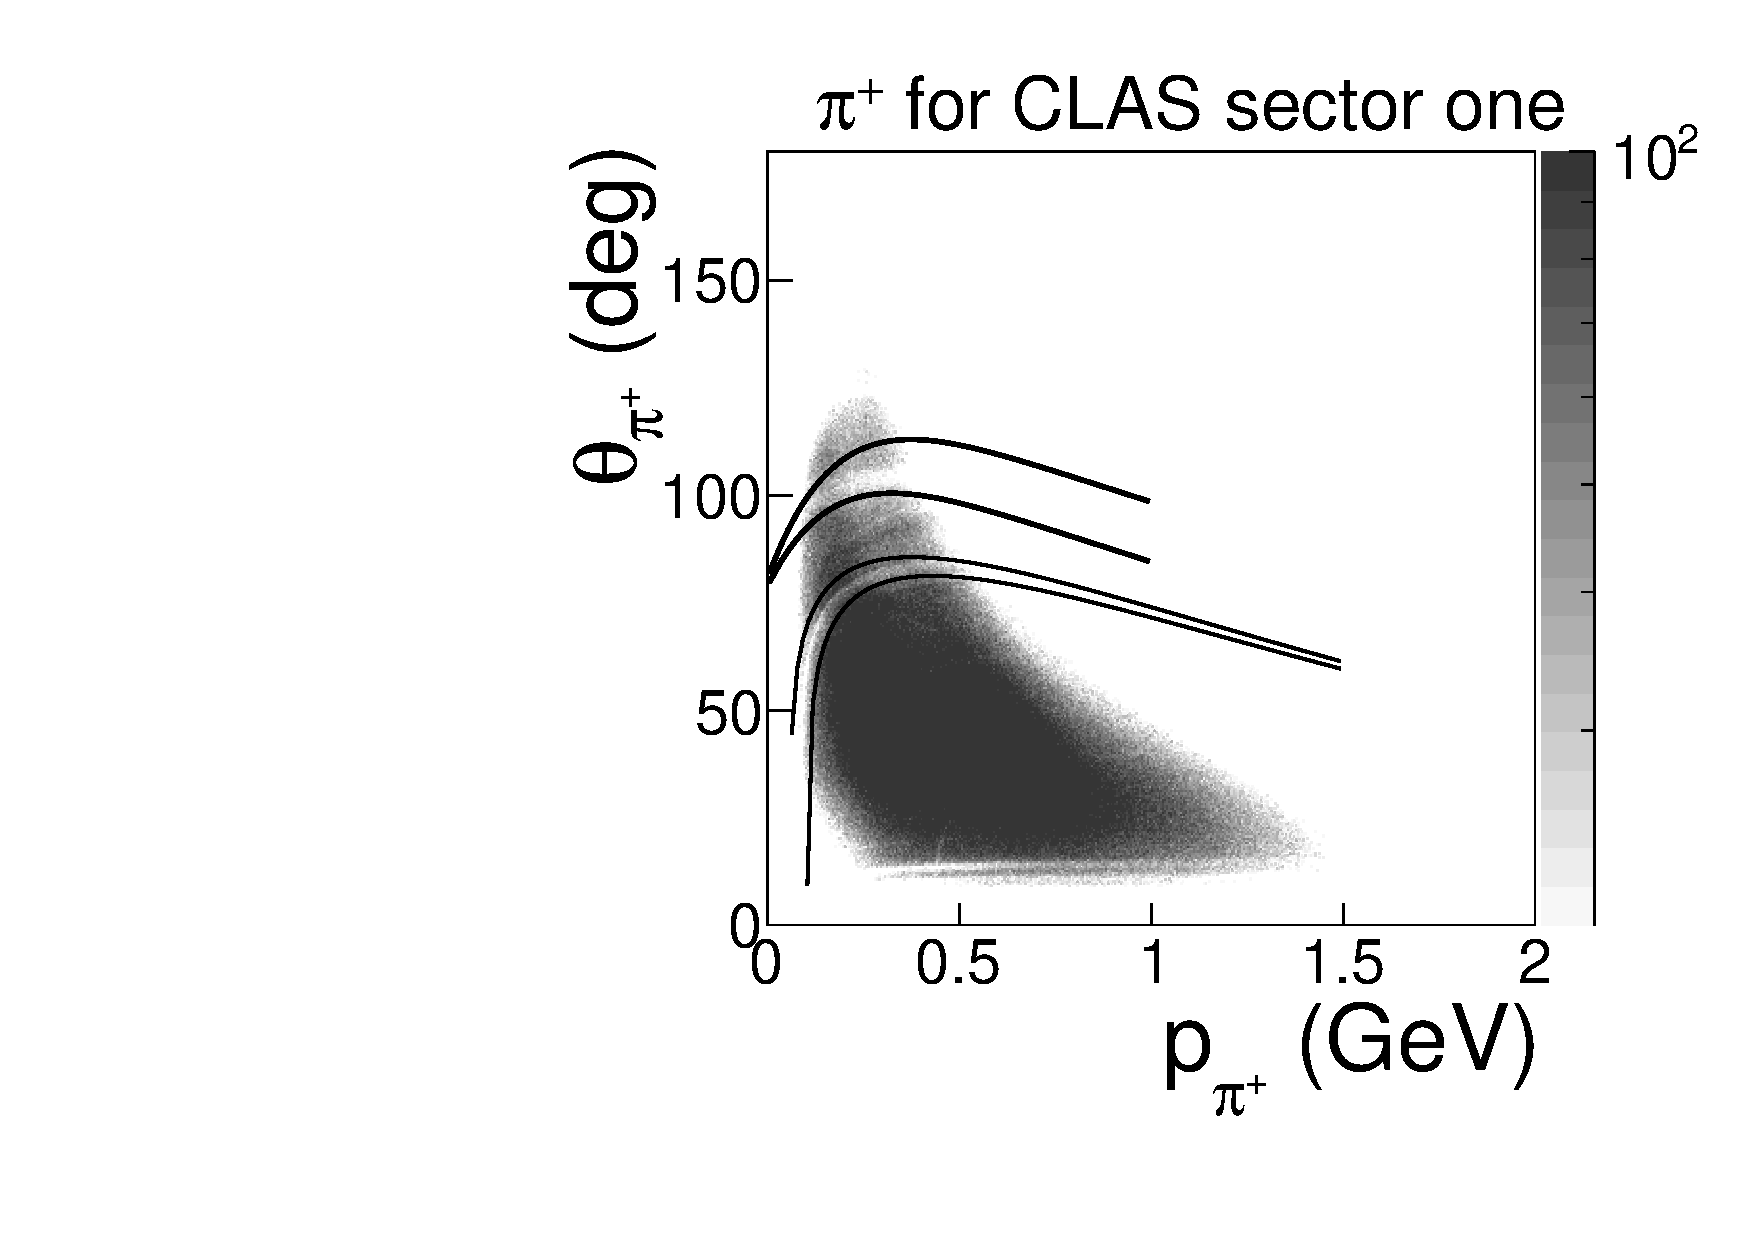
\includegraphics[width=8cm,keepaspectratio]{pictures/fiducial_cuts/th_vs_p_pip.pdf} 
\vspace{-0.1cm}
\caption{$\theta$ versus momentum distribution for $\pi^{+}$ in CLAS sector one. The angle $\theta$ is taken at the point of interaction. Black curves show the applied fiducial cuts.}
\label{fig:fid_cuts_th_vs_p}
\end{center}
\end{figure}




Some additional inefficient areas not related to the CLAS geometrical acceptance were revealed in this dataset. These areas are typicaly caused by drift chamber and time-of-flight system inefficiencies (dead wires or PMTs).  To exclude them from the consederation additional fiducial cuts on $\theta$ versus momentum distributions were applied, where $\theta$ was taken at the point of interaction.  These cuts are individual for each CLAS sector. An eaxample of the cut for $\pi^{+}$ in CLAS sector one is shown by black curves in Fig.~\ref{fig:fid_cuts_th_vs_p}. 

 


\subsubsection{Quality check cut}

\begin{figure}[htp]
\begin{center}
 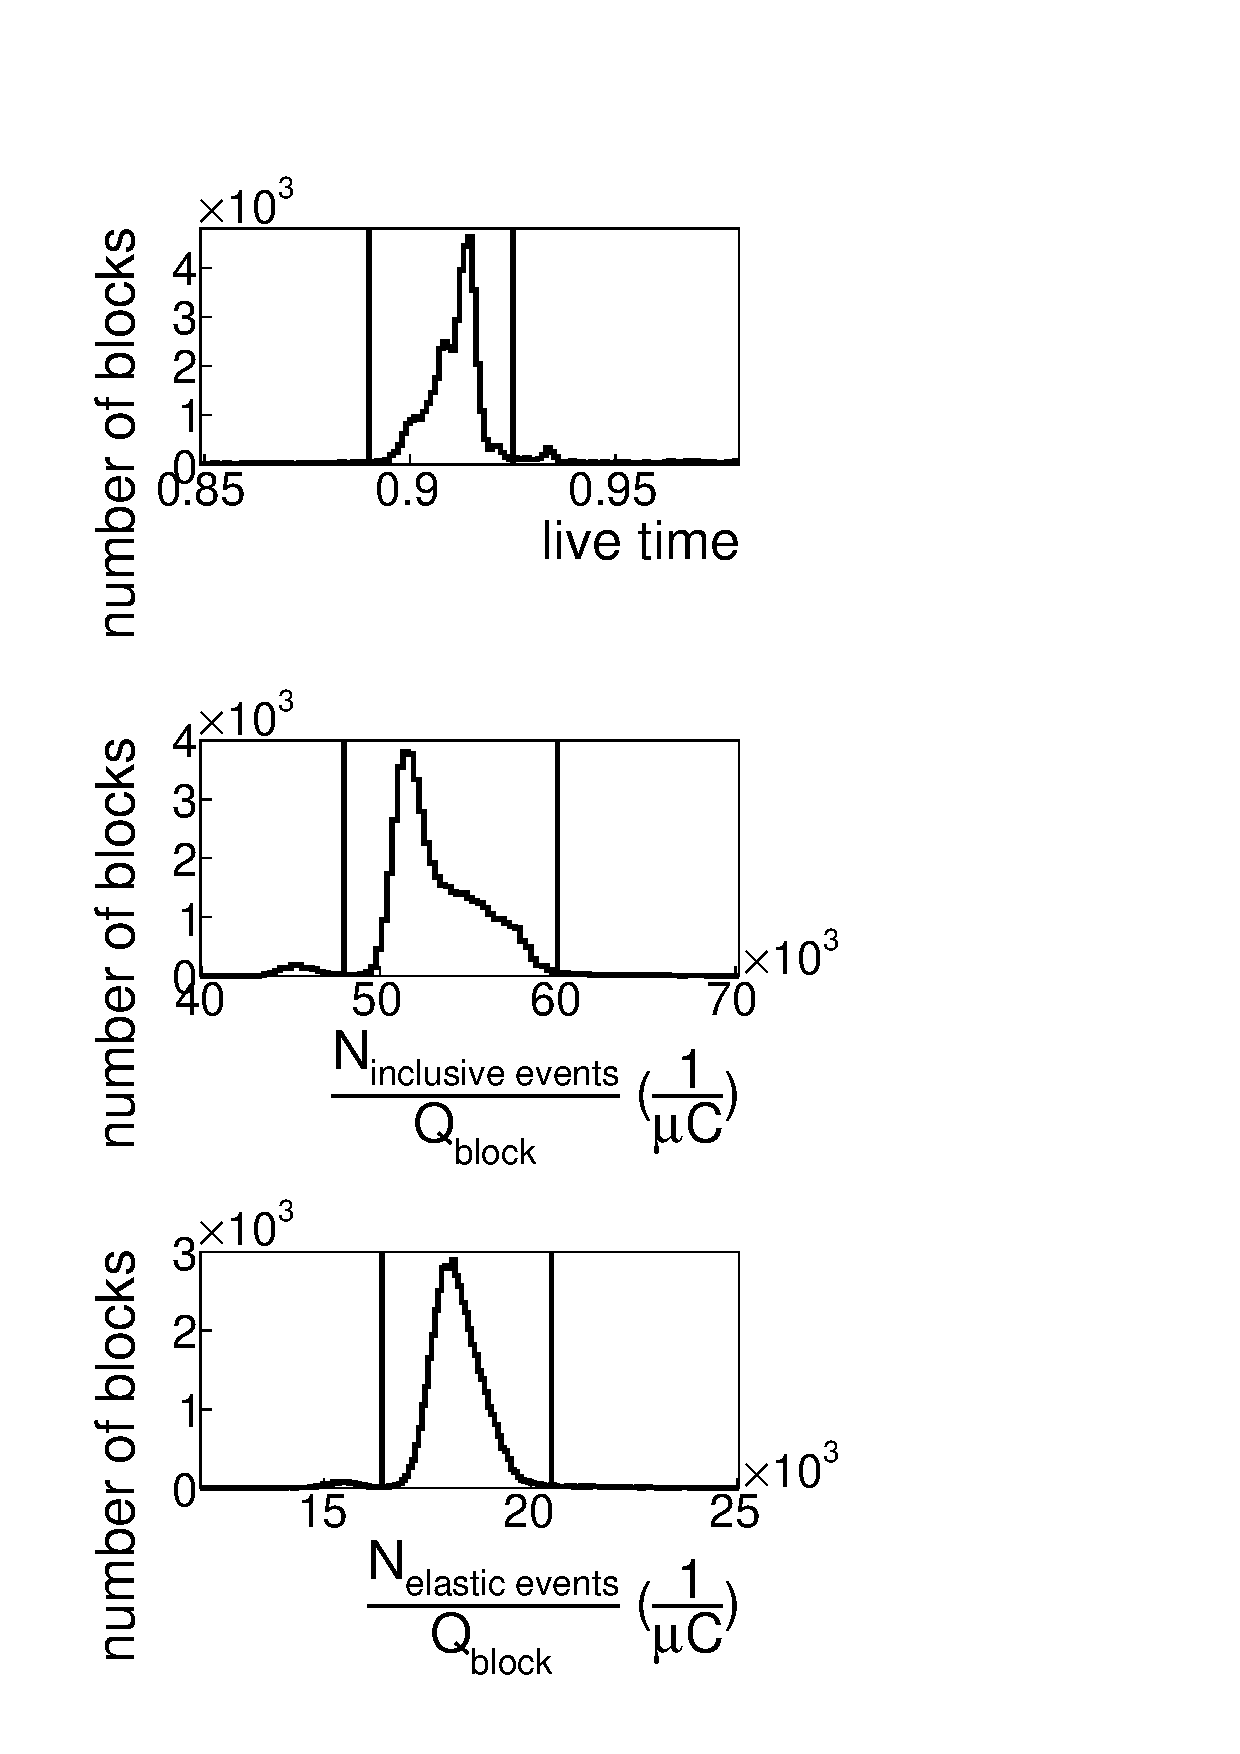
\includegraphics[width=8cm,keepaspectratio]{pictures/qcheck/qcheck1d.pdf} 
\vspace{-0.1cm}
\caption{Quality check plots. The number of blocks as functions of DAQ live time (top plot), and   yields of elastic (middle plot) and inclusive events (bottom plot) normalized to FC charge are shown. The vertical black  lines stand for the applied cuts.}
\label{fig:qcheck}
\end{center}
\end{figure} 


During the quite long experimental run the variations of the experimental conditions, like the target density deviation or improper operation of some parts of the detector, can lead to fluctuations in event yields.
 Only parts of the run with relatively stable event rates should be considered.
Therefore cuts on DAQ live time and number of events per Faraday cup (FC) charge need to be established. 

FC charge updated with a given frequency, hence the whole run time could be divided into so-called blocks. Each block corresponded to the portion of time between two FC charge readouts. The block number ranged from one to the certain maximum number over the run time. 


DAQ live time is the portion of time within the block during which the DAQ was able to accumulate events. A significant deviation of the live time from the average value indicates event rate alteration. 

In Fig.~\ref{fig:qcheck} the number of blocks is shown as functions of DAQ live time and  yields of elastic and inclusive events normalized to FC charge (from top to bottom). 
The blocks between the vertical black  lines in Fig.~\ref{fig:qcheck} were taken into the consideration.






\subsubsection{Exclusivity cut}



For picking out the reaction $e p \rightarrow e' p' \pi^{+} \pi^{-} $ it is sufficient to register at least two final hadrons along with the scattered electron. The four-momentum of the remaining unregistered hadron can be restored using the energy-momentum conservation (so-called ``the missing mass technique"). Thus one can distinguish between four so-called ``topologies" depending on the specific combination of registered final hadrons. 

\begin{enumerate}
\item $e p \rightarrow e' p' \pi^{+} X$
\item $e p \rightarrow e' p' \pi^{-} X$
\item $e p \rightarrow e' \pi^{+} \pi^{-} X$
\item $e p \rightarrow e' p \pi^{+} \pi^{-} X$
\end{enumerate}


\begin{figure}[htp!]
\begin{center}
 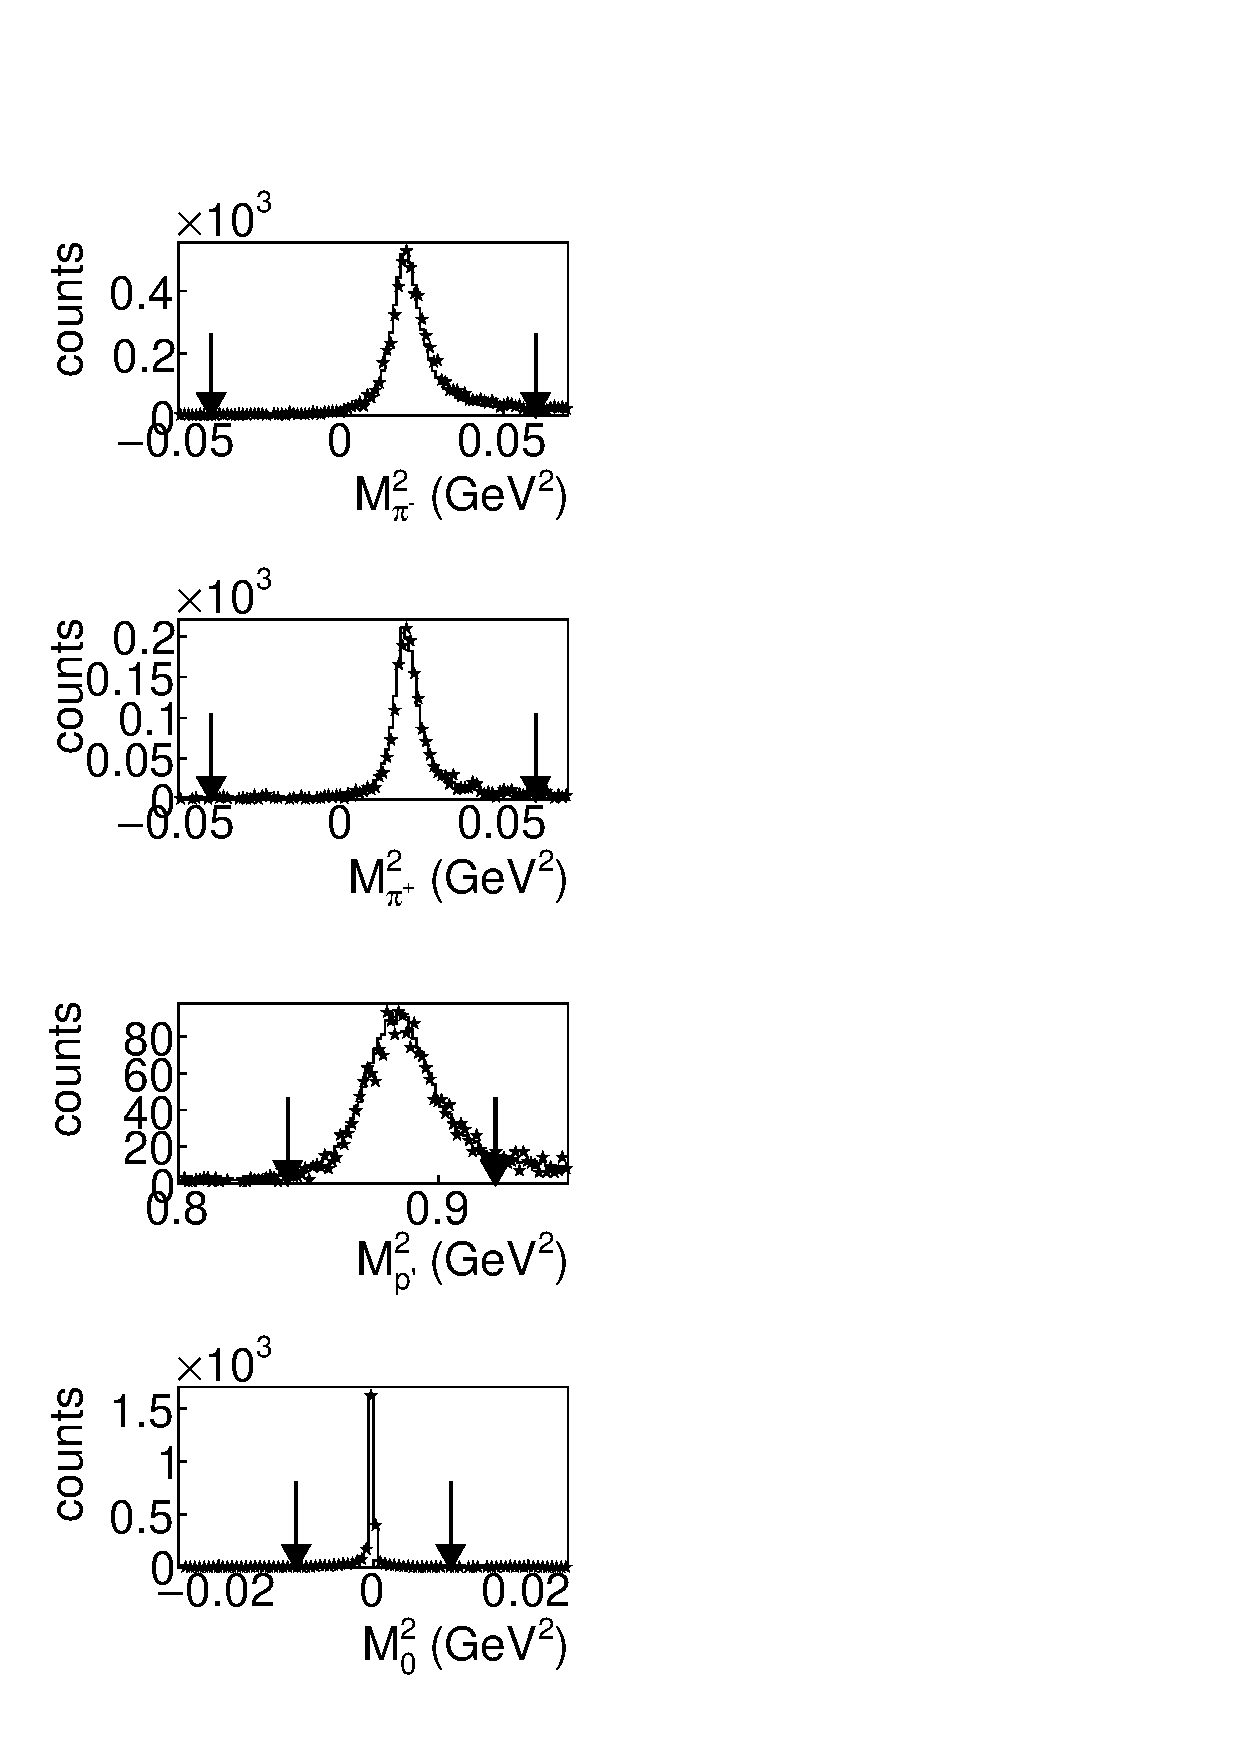
\includegraphics[width=7cm,keepaspectratio]{pictures/excl_cut/miss_mass.pdf} 
\vspace{-0.1cm}
\caption{
Missing mass squared distributions for various topologies for $1.675 < W < 1.7$~GeV in comparison with Monte Carlo. Stars show the experimental data, while curves stand for the simulation.
The plots stand for the topologies one to four from top to bottom. The arrows show the applied exclusivity cuts. 
Each distribution is normalized to the corresponded integral.}
\label{fig:miss_mass}
\end{center}
\end{figure}

Due to the experimental conditions the topology with $\pi^{-}$ missing contains about 70\% of total statistics, leaving each topology that requires $\pi^{-}$ registration to acquire only about 10\% of that. This uneven distribution of the statistics between the topologies originates from the fact that CLAS does not cover the polar angle range $0\,^{\circ}\mathrm{} < \theta_{lab} < 8\,^{\circ}\mathrm{}$ ~\cite{Me03}. 
The presence of this forward acceptance hole does not affect much the registration of the positive particles ($p$ and $\pi^{+}$), since their trajectories are bent by the magnetic field away from the hole, whereas the negative particles ($e$ and $\pi^{-}$) are inbending that means that their trajectories are bent in the forward direction. Electrons being very light and rapid undergo small track curvature and therefore the presence of the forward hole leads for them only to
the constraint on the minimal achivable $Q^2$. However, for the negative pions the situation is dramatic: being heavier and slower they are bent dominantly into the forward detector hole and, therefore, most of them can not be registered. This leads to the fact that the $\pi^{-}$ missing topology contains the dominant part of the statistics.


The topologies are defined in a way they do not overlap. For example the topology $e p \rightarrow e' p' \pi^{+} X$ requires the presence of $e'$, $p'$ and $\pi^{+}$ candidates and absence of $\pi^{-}$ candidates, avoiding in this way double counting. In most of the CLAS papers on double pion electroproduction~\cite{Isupov:2017lnd,Ripani:2002ss,Fedotov:2008aa} only topologies one and four are used. However here all four topologies are used in combination. 
This approach allows not only to slightly increase the statistics (about 20\%) but also to populate with events broader part of the reaction phase-space, since the topologies have non-identical kinematical coverage. 


%Since the topologies are different not only in statistics but also in kinematical coverage, this approach adding only about 20\% of the statistics allows to decrease model dependence of the obtained cross sections populating with events kinematical cells not avaliable in topologies one and four. 


%to increase statistics and populate with events kinematical cells not avaliable in topologies one and four.




For the case when one of the final hadrons is not registered, the missing mass $M_{X}$ for the reaction $e p \rightarrow e' h_1 h_2 X$ is determined by 



\begin{equation}
M_{X}^{2} = (P_{e} + P_{p} -P_{e'} - P_{h_1} - P_{h_2})^{2},
\label{eg:miss_mass}
\end{equation} 
where $P_{h_1}$ and $P_{h_2}$ are the four-momenta of the registered final hadrons, $P_{e}$ and $P_{p}$ - four-momenta of initial electron and proton, and $P_{e'}$ - four-momentum of the scattered electron.

While for the topology four, the missing mass $M_{X}$ for the reaction $e p \rightarrow e' p' \pi^+ \pi^- X$ is given by

\begin{equation}
M_{X}^{2} = (P_{e} + P_{p} -P_{e'} - P_{\pi^+} - P_{\pi^-} - P_{p'})^{2},
\label{eg:miss_mass_zero}
\end{equation} 
where $P_{e}$, $P_{p}$, $P_{e'}$, $P_{\pi^+}$, $P_{\pi^-}$,  and $P_{p'}$  are the four-momenta of the initial and final particles.

 


Distributions of the missing mass squared for various topologies are shown in Fig.~\ref{fig:miss_mass} for $1.675 < W < 1.7$~GeV in comparison with Monte Carlo. Stars show the experimental data, while curves stand for the simulation.
The plots in Fig.~\ref{fig:miss_mass} stand for the topologies one to four from top to bottom. The arrows show the applied exclusivity cuts. 
Each distribution in Fig.~\ref{fig:miss_mass} is normalized to the corresponded integral.

 
The Fig.~\ref{fig:miss_mass} demonstrates a good agreement between the experemental and Monte Carlo distributions,  since the simulation included both radiative effects and a background from other exclusive channels. 
The former were taken into account according to inclusive approach~\cite{Mo:1968cg}. 
The main source of the exclusive background was found to be the reaction $e p \rightarrow e' p' \pi^{+} \pi^{-} \pi^{0}$. The events for that reaction were combined with the double-pion events 
considering the ratio of three-pion/double-pion cross sections
 taken from~\cite{Wu:2005wf}. The simulation of double-pion events was carried out based on the JM05 version of double-pion production model~\cite{Ripani:2000va,Aznauryan:2005tp,Mokeev:2005re}, while for the $3\pi$ events a phase space distribution was assumed. 
 
For the purpose of the cross section calculation experimental events from all four topologies were summed up together in each multi dimentional bin. With respect to the simulation,  reconstructed Monte Carlo events were also subject to the summation.

%The $3\pi$ background can be barely seen as a separate peak on the right side of the missing mass squared distributions for the exclusive topology in last two $W$ bins (see Fig.~\ref{fig:excl_miss_mass} bottom row). For the other topologies the $3\pi$ background can not be seen as a separate peak and it manifests itself as a contribution to the tail on the right side of the missing mass squared distributions.



























%\begin{figure*}[htp]
%\begin{center}
%\frame{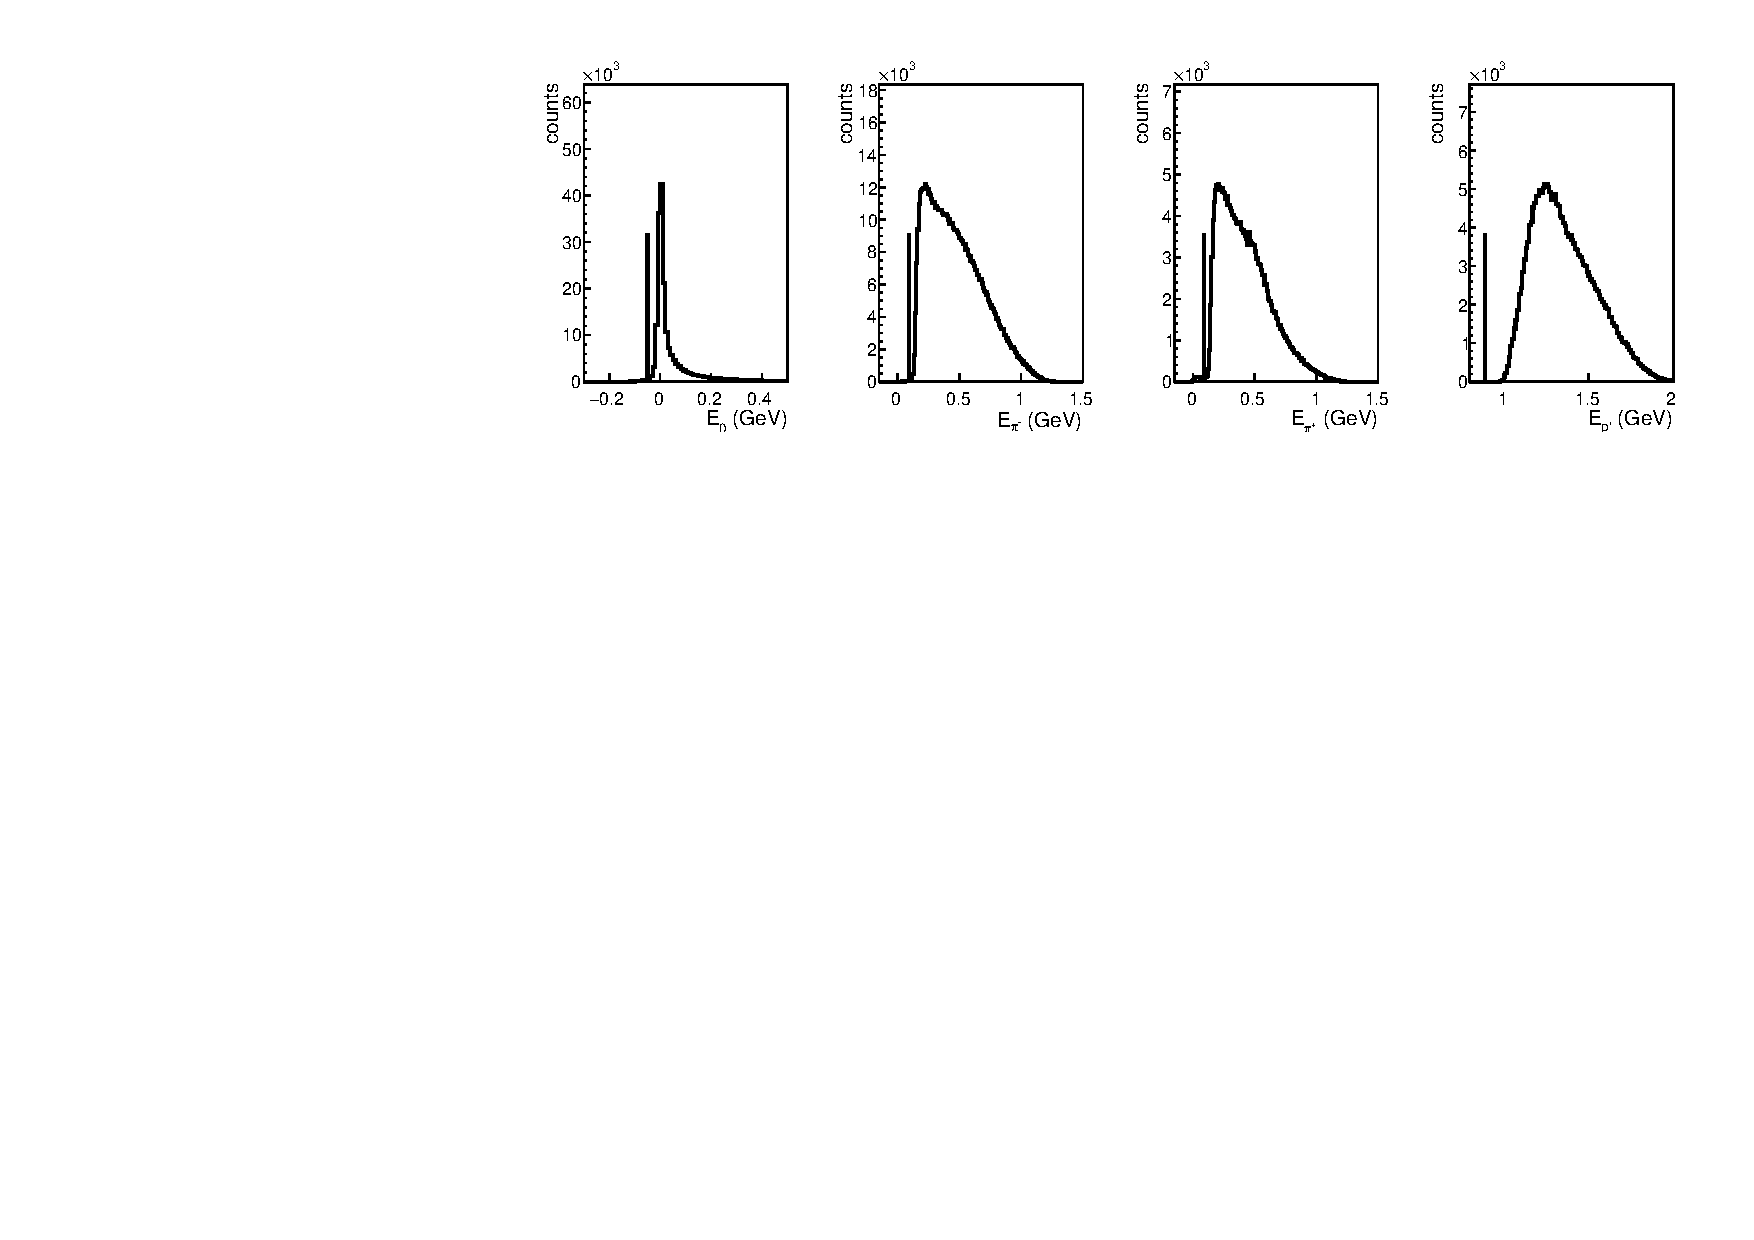
\includegraphics[width=0.95\textwidth]{pictures/miss_en/miss_en.pdf}}
%\caption{\small   Missing energy distributions for various topologies. Left plot corresponds to the topology where all final hadrons are registered and other plots correspond to the topologies with missing $\pi^-$, $\pi^+$, or proton, respectively. Vertecal lines show the applied cut. All events on the right side of the lines are selected as good for analysis.\label{fig:miss_en}}
%\end{center}
%\end{figure*}



\section{Cross section calculation}

\subsection{Kinematical variables}
\label{sec_kin_var}

Once the described above selection of the double-pion events is carried out, the four-momenta of the final hadrons are known (either registered or calculated as missing) and defined in the lab frame that corresponds to the system, where the target proton is at rest and the axis orientation is the following: $z_{lab}$ -- along the beam, $y_{lab}$ -- up, and $x_{lab}$ -- along $[\vec y_{lab} \times \vec z_{lab}]$.


The cross sections are obtained in the single-photon exchange approximation in the center of mass frame of the {\em virtual photon -- initial proton} system (c.m.s.).   
The c.m.s. is uniquely defined as the system, where the initial proton and the vitrual photon move towards each other with the axis $z_{cms}$ along the photon and the net momentum equal to zero. The axis $x_{cms}$ is situated in the elctron scattering plane, while $y_{cms}$ is along $[\vec z_{lab} \times \vec x_{lab}]$.

To transform lab system to the c.m.s. two rotations and one
boost should be perfomed~\cite{Fed_an_note:2017}.
The first rotation situates the axis $x$ in the electron scattering plane.
The second one alignes the axis $z$ with the virtual photon direction. 
Then the boost along $z$ is performed. 


To calculate the kinematical variables that describe the final hadron state the four-momenta of the final hadrons in the c.m.s. must be used.
The three-body final state is 
unambiguously determined by five kinematical
variables. 
Beside that the variables $W$ and $Q^{2}$ are needed to describe the initial state.
 
There are many ways to choose the five variables for the final hadron state description. Here the following generalized set of
variables is used~\cite{Fed_an_note:2017,Byckling:1971vca}.

\begin{itemize}
\item invariant mass of the first pair of the
hadrons $M_{h_{1}h_{2}}$;
\item invariant mass of the second pair of the
hadrons $M_{h_{2}h_{3}}$;
\item the first hadron solid angle $\Omega_{h_{1}} = (\theta_{h_{1}}, \varphi_{h_{1}})$;
\item the angle $\alpha_{h_{1}}$ between two planes: one of
them is defined by the three-momenta of
the virtual photon (or initial proton) and the first final hadron, the second
plane is defined by the three-momenta of all final hadrons (see Appendix~\ref{app_a}).
\end{itemize}

%\afterpage{\clearpage}

The cross sections  were obtained in three sets of variables depending on
various assignments for the first, second, and
third final hadrons:

\begin{enumerate}
\item $\boldsymbol{first\; - p',\; second \; - \pi^{+},\; third - \pi^{-}}$: \\ $M_{p'\pi^{+}}$, $M_{\pi^{+}\pi^{-}}$, $\theta_{p'}$, $\varphi_{p'}$,  $\alpha_{p'}$ (or $\alpha_{(p,p')(\pi^{+},\pi^{-})}$);
\item $\boldsymbol{first\; - \pi^{-},\; second \; - \pi^{+},\; third - p'}$: $M_{\pi^{-}\pi^{+}}$, $M_{\pi^{+}p'}$, $\theta_{\pi^{-}}$, $\varphi_{\pi^{-}}$, $\alpha_{\pi^{-}}$ (or $\alpha_{(p\pi^{-})(p'\pi^{+})}$ ) and
\item $\boldsymbol{first\; - \pi^{+},\; second \; - \pi^{-},\; third - p'}$: $M_{\pi^{+}\pi^{-}}$, $M_{\pi^{-}p'}$, $\theta_{\pi^{+}}$, $\varphi_{\pi^{+}}$, $\alpha_{\pi^{+}}$ (or $\alpha_{(p\pi^{+})(p'\pi^{-})}$ ).
\end{enumerate}







\subsection{Binning and kinematical coverage}

The kinematical coverage in the initial state variables is shown by the $Q^{2}$ versus $W$ distribution in Fig. \ref{fig:q2vsw}. The color code of the distribution represents the number of exclusive double-pion events left after the cuts and corrections described above. 
The white boundary limits the kinematical area, where the double-pion cross sections were extracted. The black grid demonstates the chosen binning in the initial state variables. 



\begin{figure}[htp]
\begin{center}
 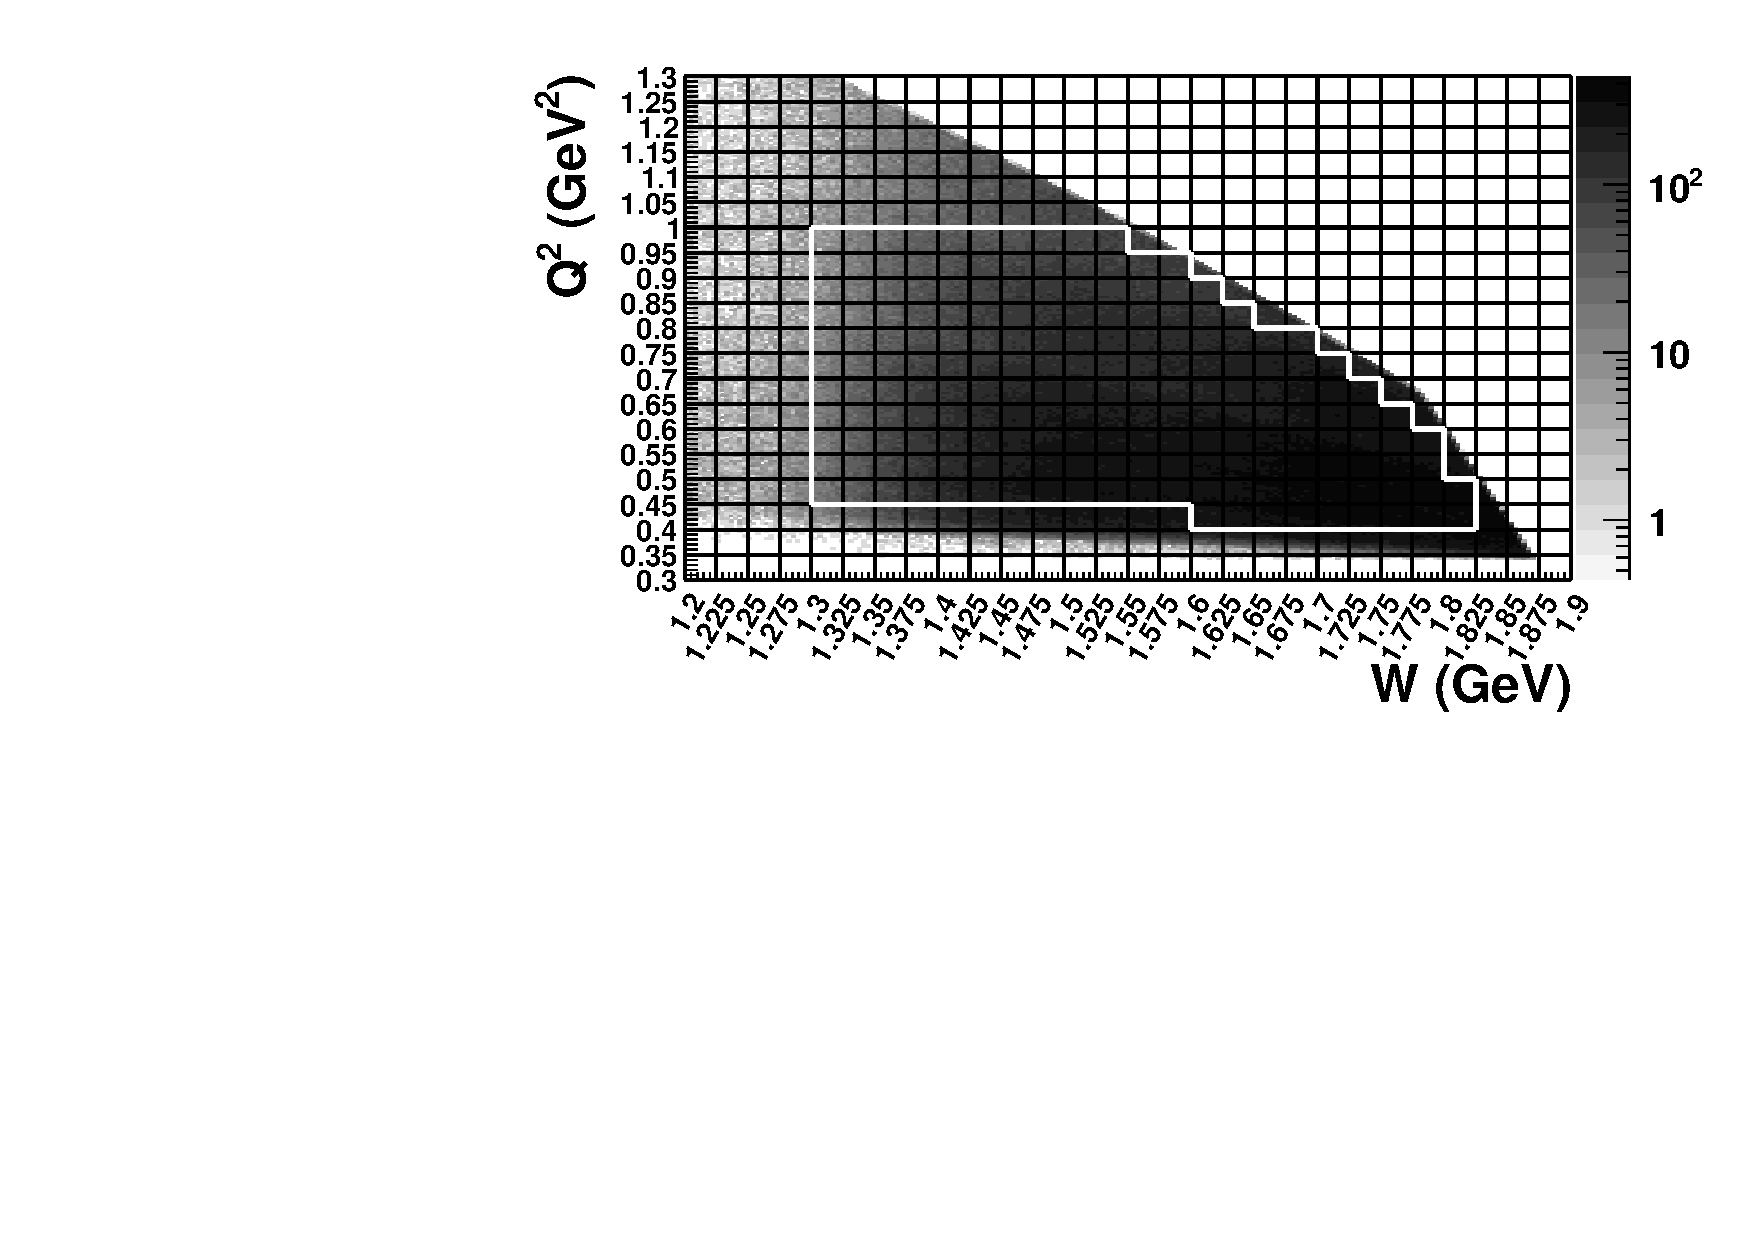
\includegraphics[width=8.5cm,keepaspectratio]{pictures/binning/q2vsw.pdf} 
\vspace{-0.1cm}
\caption{$Q^2$ versus $W$ distribution populated with selected double-pion events. The cross section was calculated in 2D cells within the white boundaries.}
\label{fig:q2vsw}
\end{center}
\end{figure} 

The binning in the final hadron variables is listed in Tab.~\ref{tab:summary_bins}. It is chosen to maintain the resonable statistical uncertanties in all $W$ and $Q^{2}$ bins. The binning choice also takes into account the cross section drop near the double-pion production threshold at $\approx 1.22$~GeV as well as the broadening of the reaction phase space with increase of $W$. 

The binning in invariant masses requires a special attention.
As it is shown in Eq.~\ref{eq:inv_mass_boundary} the left boundary of the invariant mass distributions is fixed, while the right one grows with $W$. 
\begin{equation}
\begin{aligned}
M_{left} & = m_{h1} + m_{h_2} \\
M_{right} & = W_{center} - m_{h_3}, \label{eq:inv_mass_boundary}
\end{aligned}  
\end{equation}
where $M_{left}$ and $M_{right}$ are the left and right boundaries of  the invariant mass distribution. $m_{h_1}$, $m_{h_2}$, and $m_{h_3}$ are the masses of the final hadrons. The value of $W_{center}$ is taken at the center of the corresponding bin $W_{left} < W < W_{right}$ , since the exctracted cross section is assumed to be assigned to the center of a bin.

%It leads to the fact that invariant mass distributions are broader at high $W$ and hence a more detailed binning in that area is necessary (see Tab.~\ref{tab:summary_bins}).

\begingroup
\squeezetable
\begin{table}[htp]
\centering 

\begin{tabular}{|c|C{0.065\textwidth}|C{0.065\textwidth}|C{0.075\textwidth}|C{0.09\textwidth}|}
\hline \multirow{2}{*}{\diagbox[width=2.9cm, height=1.cm]{\raisebox{2.5pt}{$W$ range}}{\raisebox{-3pt}{Variable}}} & Number of bins in invariant mass $M$ &Number of  bins in polar angle $\theta$ &Number of bins in  azimuthal angle $\varphi$ &Number of bins in angle between two planes $\alpha$ \\
\hline
 1.3 - 1.35 GeV & 8 & 6 & 5 & 5\\
\hline
1.35 - 1.4 GeV & 10 & 8 & 5 & 6\\
\hline 
 1.4 - 1.45 GeV & 12 & 10 & 5 & 8\\
\hline 
 $ > 1.45$ GeV & 12 & 10 & 8 & 8\\
\hline 
\end{tabular}
\caption{\small Number of bins for the given final hadron variables. \label{tab:summary_bins}}
\end{table}
\endgroup

\begin{figure}[htp]
\begin{center}
\frame{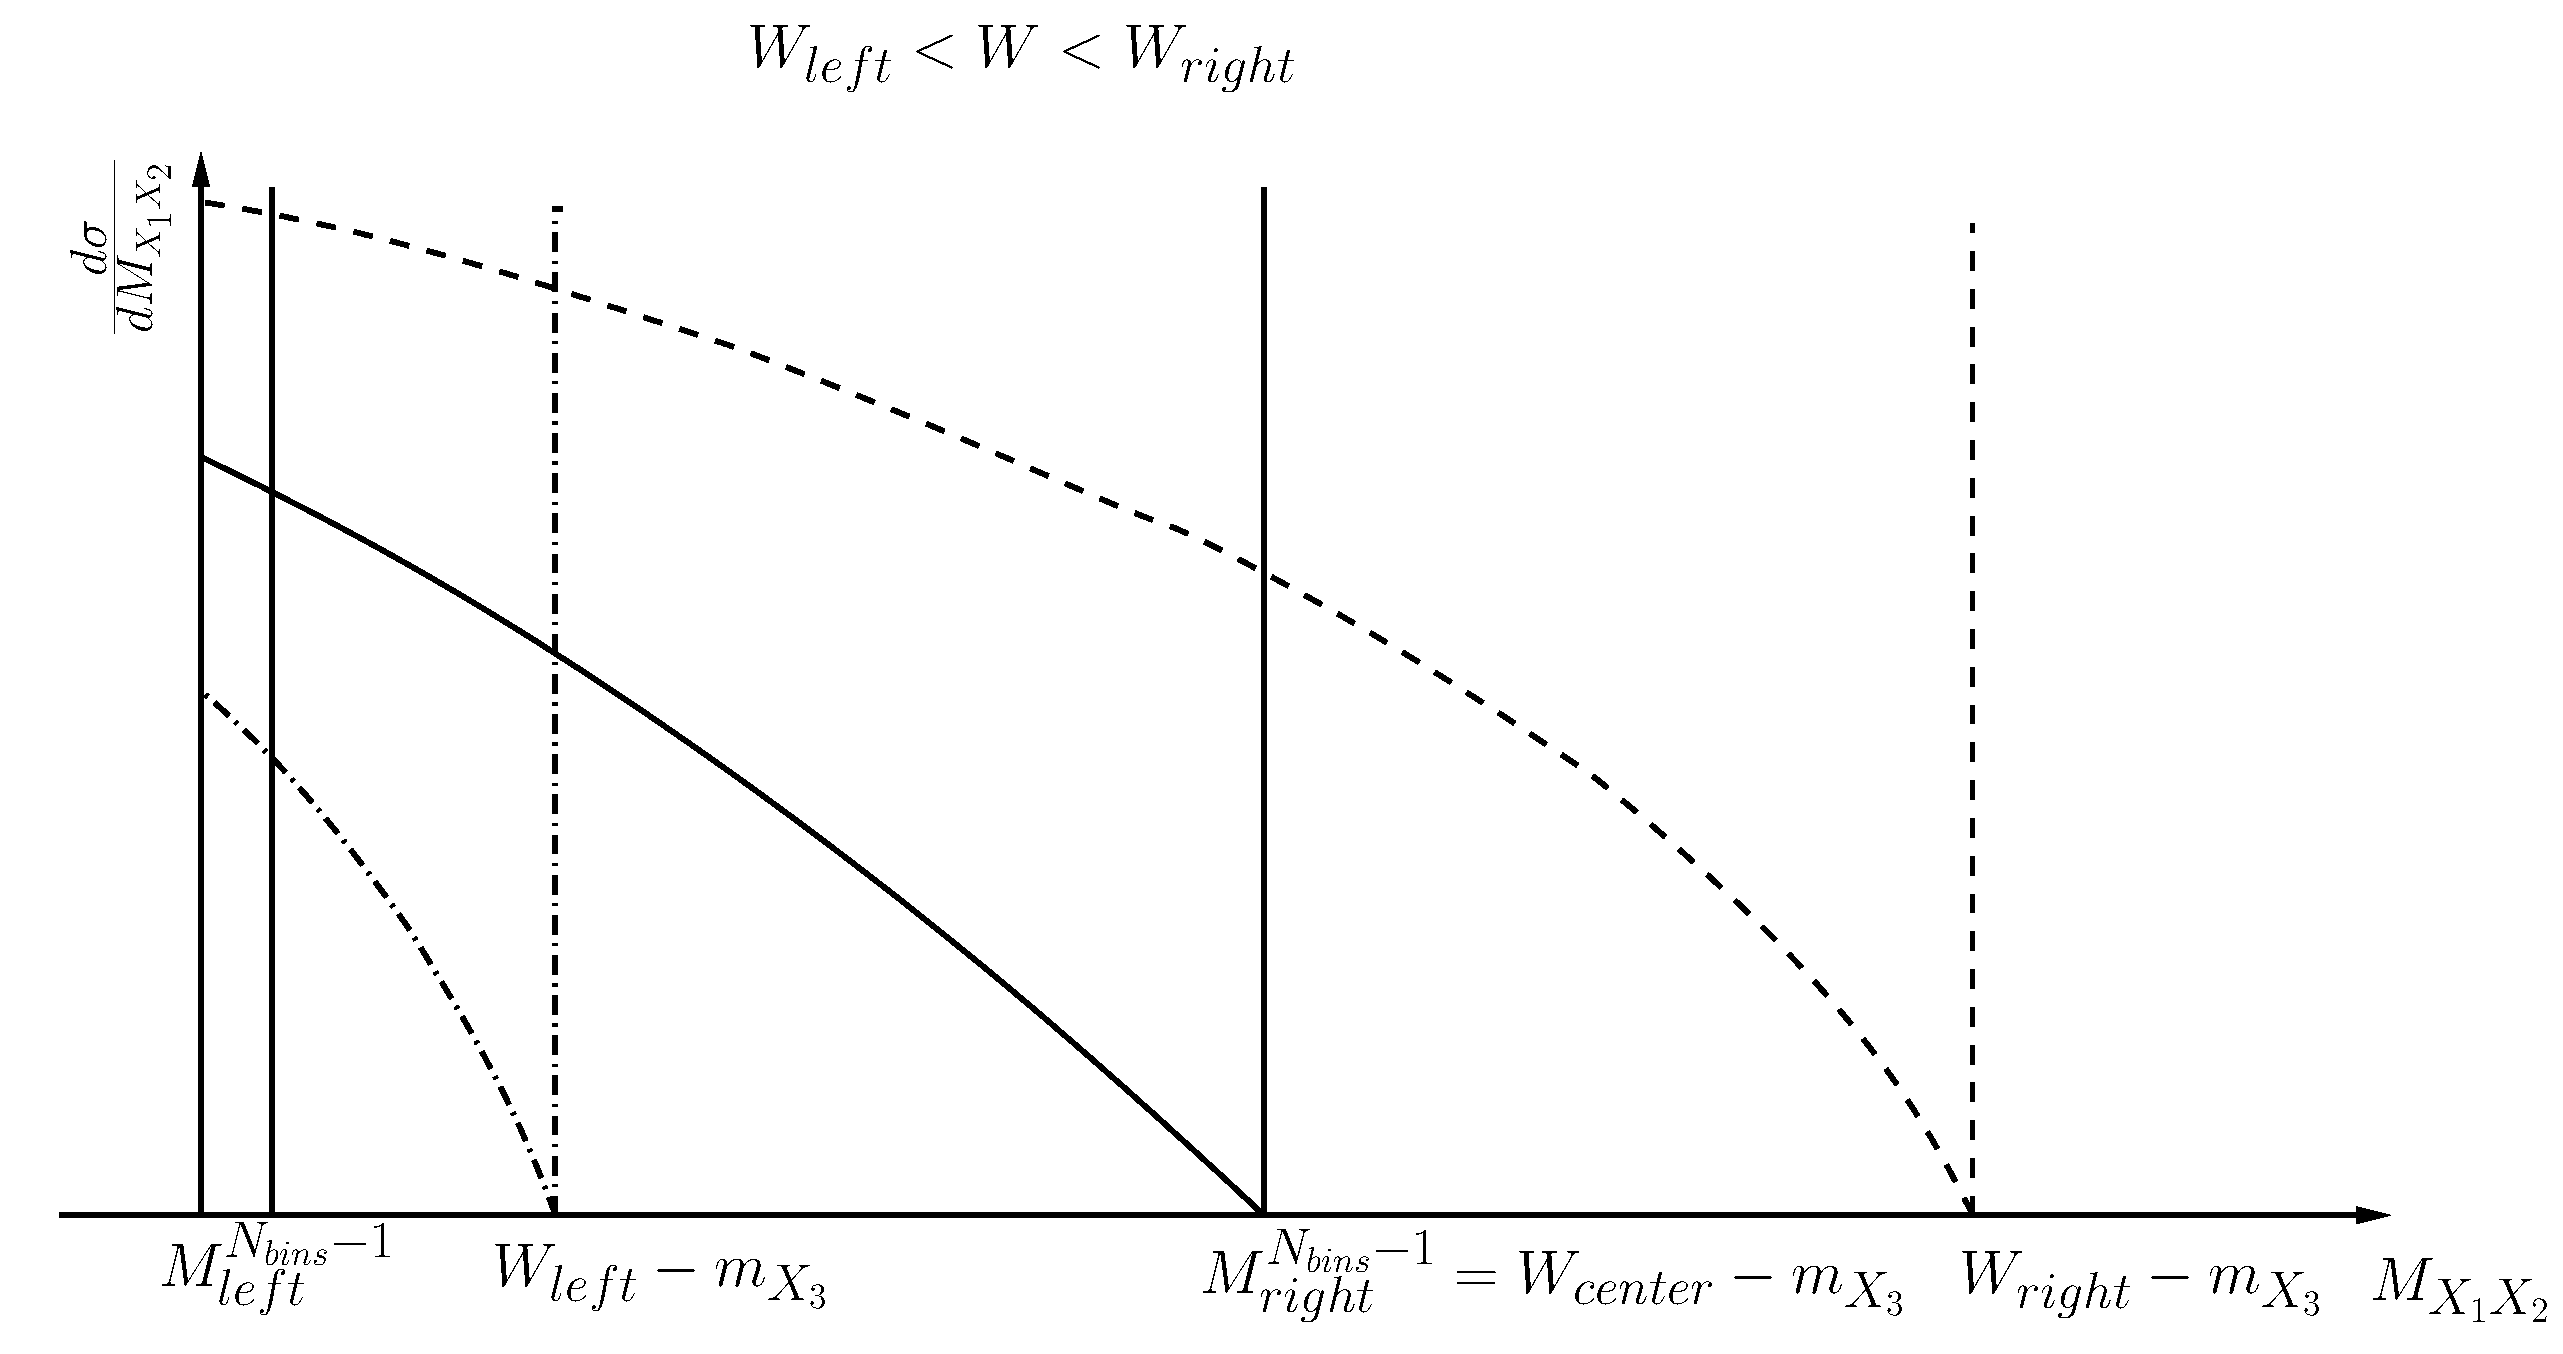
\includegraphics[width=8cm]{pictures/mass_corr/mass_tex.pdf}}
\caption{\small Schematic representation of the cross sections in the next to last bin in the invariant mass $(M_{h_{1}h_{2}})$ for various $W$. Dot-dashed and dashed vertical lines show  maximal invariant mass values that can be reached with $W_{left}$ and $W_{right}$, respectively, while vertical black  lines show the boundaries of the next to last bin in the invariant mass.  \label{fig:mass_corr}}
\end{center}
\end{figure}

All events from the range $W_{left} < W < W_{right}$ contribute to the invariant mass distributions. Since
the right boundary of these distributions  is calculated using $W_{center}$ some events turned out to be located beyond $M_{right}$. 
Hence it was decided to use the following specific arrangment of bins.
 Firstly the bin width $\Delta M$ is determined as:
\begin{equation}
\begin{aligned}
\Delta M = \frac{M_{right}-M_{left}}{N_{bins}-1}, \label{eq:bin_width}
\end{aligned}  
\end{equation} 
where $N_{bins}$ is the number of the bins specified in Tab.~\ref{tab:summary_bins}. 

Then the invariant mass distributions are obtained within the limits from $M_{left}$ to $M_{right}+\Delta M$ causing the last bin to be situated completely out of the boundaries given by Eq.~\ref{eq:inv_mass_boundary}. Although the cross section obtained in this bin is very small, this bin is however kept since its content contributes to all other cross sections obtained by integration over the corresponding invariant mass. 
After the binning corrections this effect is assumed to be taken into account and this last bin in invariant masses is neglected. 

The cross section in the next to last bin should be treated carefully.
In Fig.~\ref{fig:mass_corr} the distributions of the invariant mass $M_{h_{1}h_{2}}$ are schematically illustrated for three values of $W$, i.e. $W_{left}$ -- dot-dashed curve, $W_{center}$ -- solid curve, and $W_{right}$ -- dashed curve. 
The dot-dashed and dashed vertical lines show  maximal invariant mass values that can be reached with $W_{left}$ and $W_{right}$, respectively, while the vertical black solid lines show the boundaries of the next to last bin in the invariant mass.
The invariant mass distributions for $W$ from $W_{left}$ to $ W_{center}$  have the right edges within this bin.
As a consequence events that contribute to the next to last bin are distributed in the range, which is less than invariant mass bin width $\Delta M$ defined by Eq.~\ref{eq:bin_width}. Since on a level of cross section extraction the bin width $\Delta M$ given by Eq.~\ref{eq:bin_width} is always used this effect leads to the cross section underestimation.



The correction for this effect is made using TWOPEG double pion event generator~\cite{Skorodum:EG}. For that purpose for each invariant mass two  one-dimensional distributions are generated in each $W$ bin. The first one mimics the data distribution, for which all events in the next to last bin are divided by the same bin width $\Delta M$.  For the second one events with $W$ between $W_{center}$ and $W_{right}$ are divided by $\Delta M$, while events with $W$ between $W_{left}$ and $W_{center}$ are divided by the bin width that is individual for each event and equal to $W - m_{h_{3}} - M_{left}^{N_{bins}-1}$, where $M_{left}^{N_{bins}-1}$ is the left boundary of the nex to last bin (see left solid vertical line in Fig.~\ref{fig:mass_corr}). The correction factor, by which obtained single-differential cross sections in the next to last bin should be multiplied, is defined as the ratio of the second distribution over the first one. This factor provides the correction to the cross section in the nex two last bin that varies from 5\% to 10\%. 

























\subsection{Cross section formula}
\label{cr_sect_formula}


In the single photon exchange approximation the virtual photoproduction cross section $\sigma_{v}$ is connected with the experimental electron scattering cross section $\sigma_{e}$ via Eq.~\eqref{fulldiff}. 

\begin{equation}
\begin{aligned}
\frac{d^{5}\sigma_{v}}{d^{5}\tau} & = \frac{1}{\Gamma_{v}}
\frac{d^{7}\sigma_{e}}{dWdQ^{2}d^{5}\tau}; \\
d^{5}\tau & = dM_{h_{1}h_{2}}dM_{h_{2}h_{3}}d\Omega_{h_{1}}
d\alpha_{h_{1}} \textrm{ ,}
\label{fulldiff}
\end {aligned}
\end{equation}
where $d^{5}\tau$ is the differential of the five independent variables of the final $\pi^{+}\pi^{-}p$, which were described in Sec.~\ref{sec_kin_var}, $\Gamma_{v}$ is the 
virtual photon flux, given by

\begin{equation}
\Gamma_{v}(W,Q^{2}) =
\frac{\alpha}{4\pi}\frac{1}{E_{beam}^{2}m_{p}^{2}}\frac{W(W^{2}-m_{p}^{2})}
{(1-\varepsilon_{T})Q^{2}} \textrm{ ,}
\label{flux}
\end{equation}
where $\alpha$ is the fine structure constant $\left(1/137\right)$, $m_{p}$ is the proton
mass, $E_{beam} = 2.039$~GeV is the energy of the incoming electron beam, and $\varepsilon_{T}$ is the virtual photon transverse polarization, given by

\begin{equation}
\varepsilon_{T} = \left( 1 + 2\left( 1 +
\frac{\nu^{2}}{Q^{2}} \right)
tan^{2}\left(\frac{\theta_{e'}}{2}\right) \right)^{-1} \textrm{ ,}
\label{polarization}
\end{equation}
where $\nu = E_{beam} - E_{e'}$ is the virtual photon energy, while $E_{e'}$ and
$\theta_{e'}$ are the energy and the polar angle of the scattered electron in the
lab frame, respectively. 
%$W$, $Q^{2}$ and $\theta_{e'}$ are
%taken in the center of the bin.

The experimentalelectron scattering cross section $\sigma_{e}$ introduced in Eq.~\eqref{fulldiff} in turn can be calculated as
  
 
\begin{equation}
\frac{d^{7}\sigma_{e}}{dWdQ^{2}d^{5}\tau} = \frac{1}{F \cdot R} 
\frac{\left( \frac{\Delta N_{full}}{Q_{full}}-\frac{\Delta N_{empty}}{Q_{empty}} \right)}{
\Delta W \Delta Q^{2} \Delta^{5} \tau \left( \frac{l \rho N_{A}}{q_{e}M_{H}} \right)} \textrm{ ,}
\label{expcrossect}
\end{equation}
where $\Delta N_{full}$ and $\Delta N_{empty}$ are the numbers of selected double-pion events inside the
seven-dimensional bin for runs with hydrogen and
empty target, respectively. 
Each event is weighted with the corresponding photoelectron correction factor given by Eq.~\ref{eq:cc_corr_fact}.
 $F = F(\Delta W, \Delta Q^{2}, \Delta \tau)$ is the detector efficiency for the seven-dimensional bin
 coming from the  Monte Carlo simulation,
$R = R(\Delta W, \Delta Q^{2})$ is the
radiative correction factor described in Sec.~\ref{rad_corr},  $Q_{full}= 5999.64$~$\mu$C and $Q_{empty} = 334.603$~$\mu$C are the  values of the charge accumulated on the Faraday cup for runs with hydrogen and empty target, respectively. $q_{e} =1.610^{-19}$ C is the elementary charge, $\rho = 0.0708$  g/cm$^{3}$ is the density of liquid hydrogen at $T = 20$~K,
$l = 2$ cm is the length of the target, $M_{H} = 1.00794$ g/mol is the molar density of
the natural mixture of hydrogen,  $N_{A} =6.0210^{23}$ mol$^{-1}$ is Avogadro's
number.

%Infinitesimal differentials in the left hand side of Eq.~\ref{expcrossect} 
The electron scattering cross section in the left hand side of Eq.~\ref{expcrossect} is assumed to be obtained in the center of the finite seven-dimentional kinematical bin $\Delta W \Delta Q^{2} \Delta^{5} \tau$.





The limited
statistics of the experiment does not allow to estimate
the five-differential cross section $\sigma_{v}$ with the reasonable
accuracy. Therefore being obtained on the multi-dimentional grid, the cross section $\sigma_{v}$ is futher integrated over all hadron variables except of one. Hence only the sets of the single-differential and fully integrated cross sections are presented as a result here.

For each bin in $W$ and $Q^2$ the following cross sections are obtained
\begin{equation}
\begin{aligned}
\frac{d\sigma}{dM_{h_{1}h_{2}}} & =
\int\frac{d^{5}\sigma}{d^{5}\tau}dM_{h_{2}h_{3}}d\Omega_{h_{1}}d\alpha_{h_{1}};  \\
\frac{d\sigma}{dM_{h_{2}h_{3}}} & =
\int\frac{d^{5}\sigma}{d^{5}\tau}dM_{h_{1}h_{2}}d\Omega_{h_{1}}d\alpha_{h_{1}}; \\
\frac{d\sigma}{d(-cos\theta_{h_{1}})} & =
\int\frac{d^{5}\sigma}{d^{5}\tau}dM_{h_{1}h_{2}}dM_{h_{2}h_{3}}d\varphi_{h_{1}}d\alpha_{h_{1}};  \\
\frac{d\sigma}{\alpha_{h_{1}}} & =
\int\frac{d^{5}\sigma}{d^{5}\tau} dM_{h_{1}h_{2}}dM_{h_{2}h_{3}}d\Omega_{h_{1}}; \\
\sigma_{int}(W,Q^{2}) & =
\int\frac{d^{5}\sigma}{d^{5}\tau}dM_{h_{1}h_{2}}dM_{h_{2}h_{3}}d\Omega_{h_{1}}d\alpha_{h_{1}}.
\end{aligned}
\label{inegr5diff}
\end{equation}

Since the cross sections are obtained on the
five-dimensional kinematical grid,
integrals in~(\ref{inegr5diff}) are calculated numerically 
on that grid. 

%For other sets of kinematical variables single-fold differentional cross sections were determined in the same way.







\subsection{Efficiency evaluation}
\label{eff_err}

For the Monte Carlo simulation the GENEV event generator developed by 
Genova group was used. This event generator uses the JM05 model~\cite{JM05} for the investigated double-pion channel,
while for the background channel $e p \rightarrow e'p'\pi^{+}\pi^{-}\pi^{0}$, which was generated along with the main one, GENEV assumes the phase space distributions for all kinematical variables.



\begin{figure}[htp]
\begin{center}
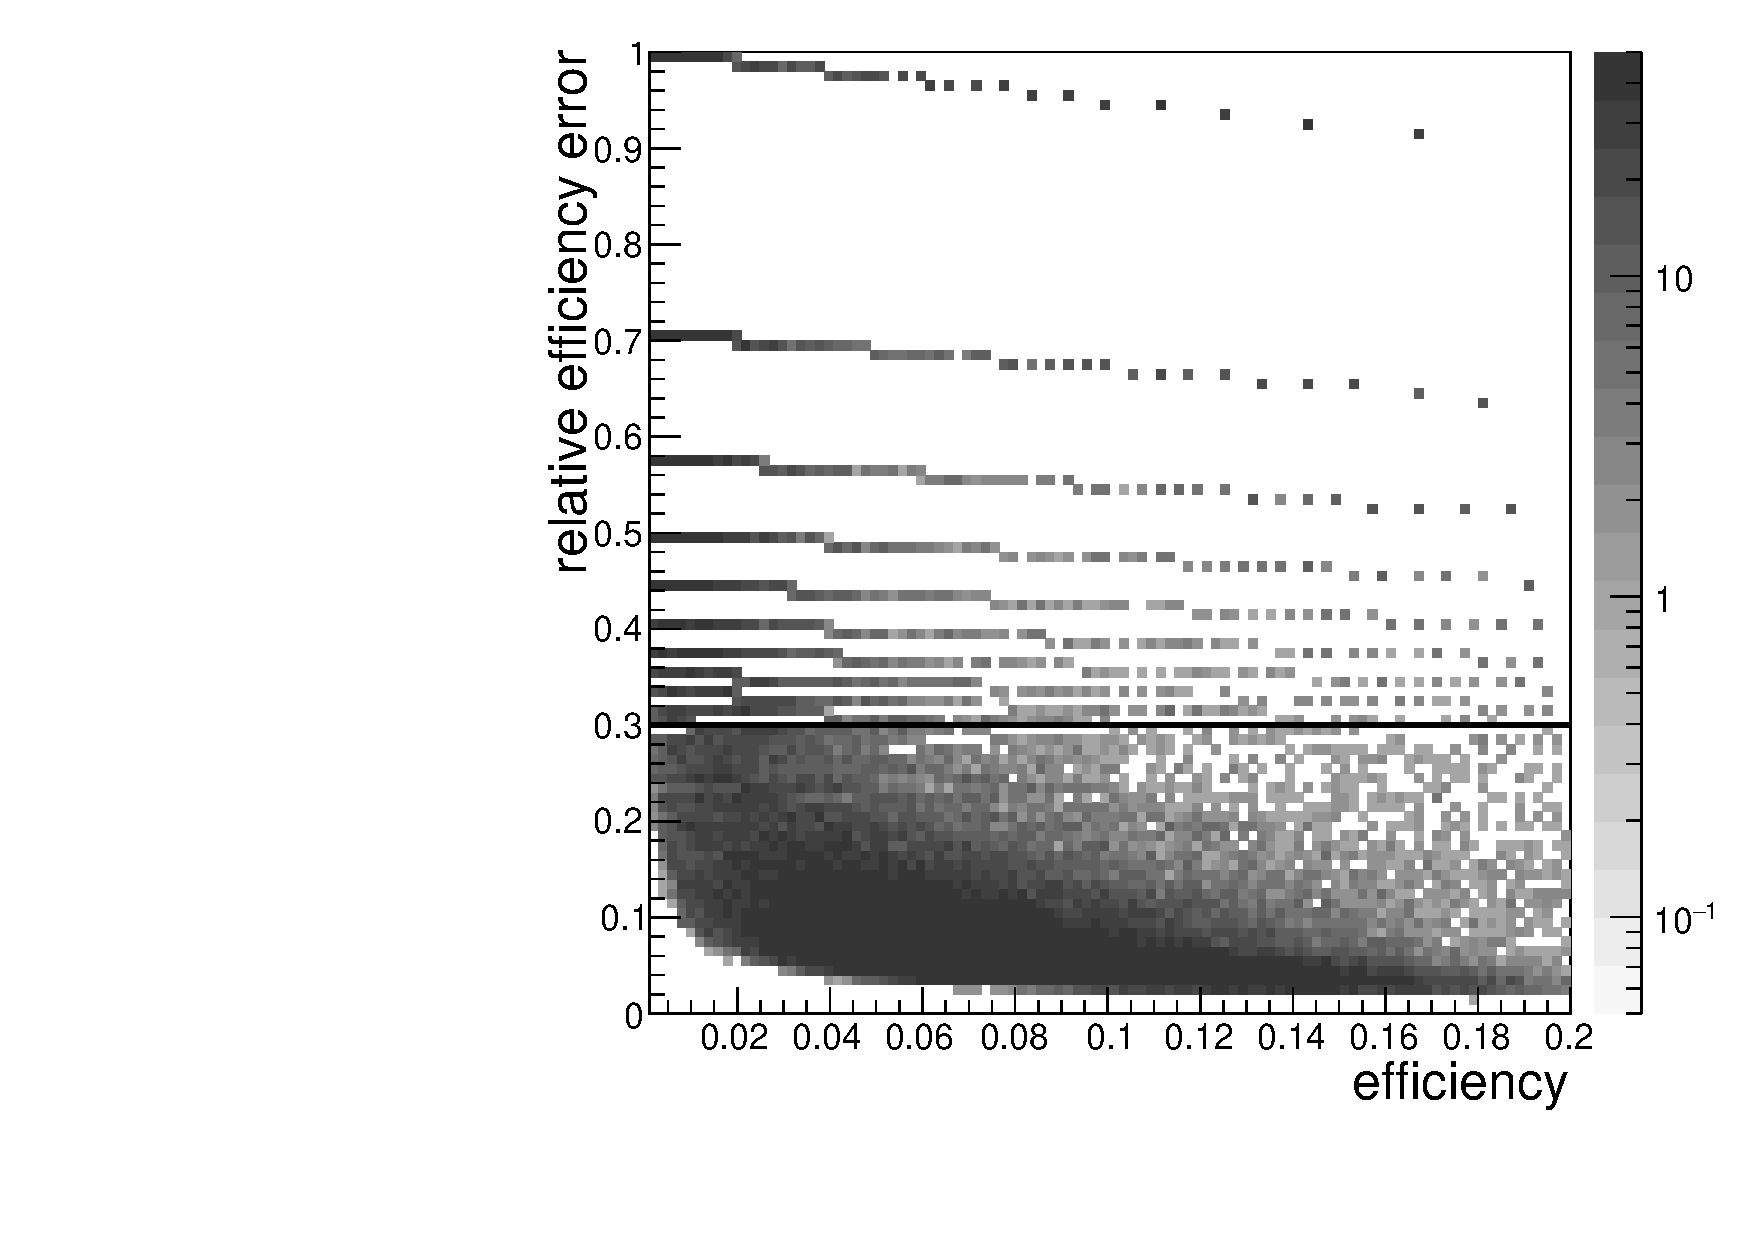
\includegraphics[width=7cm]{pictures/efficiency/eff_err.pdf}
\caption{\small Relative efficiency error versus efficiency for one particular bin in $W$ and $Q^2$ ($W = 1.6375$~GeV, $Q^2 = 0.525$~GeV$^2$). Color code shows the number of five-dimensional cells.} \label{fig:eff_err}
\end{center}
\end{figure}

The generated events were passed through the GEANT based detector siumulation and reconstruction procedures. Then the efficiency factor $F$ from Eq.~\eqref{expcrossect} is calculated in each $\Delta W\Delta Q^{2}\Delta^{5} \tau$ bin as:
\begin{equation}
F(\Delta W, \Delta Q^{2}, \Delta^{5} \tau) = \frac{N_{rec}}{N_{gen}},
\label{efficiency}
\end{equation}
where $N_{gen}$ is the number of generated double-pion events inside the multi-dimensional bin, while $N_{rec}$ is the number of reconstructed either double- and three-pion events survived in that bin after the event selection. This definition of the efficiency factor $F$ allows to account for the three-pion background that is negligible at $W < 1.6$ GeV  and
grows up to a few percent at $W \approx 1.8$ GeV. 

\begin{figure*}[htp]
\begin{center}
\frame{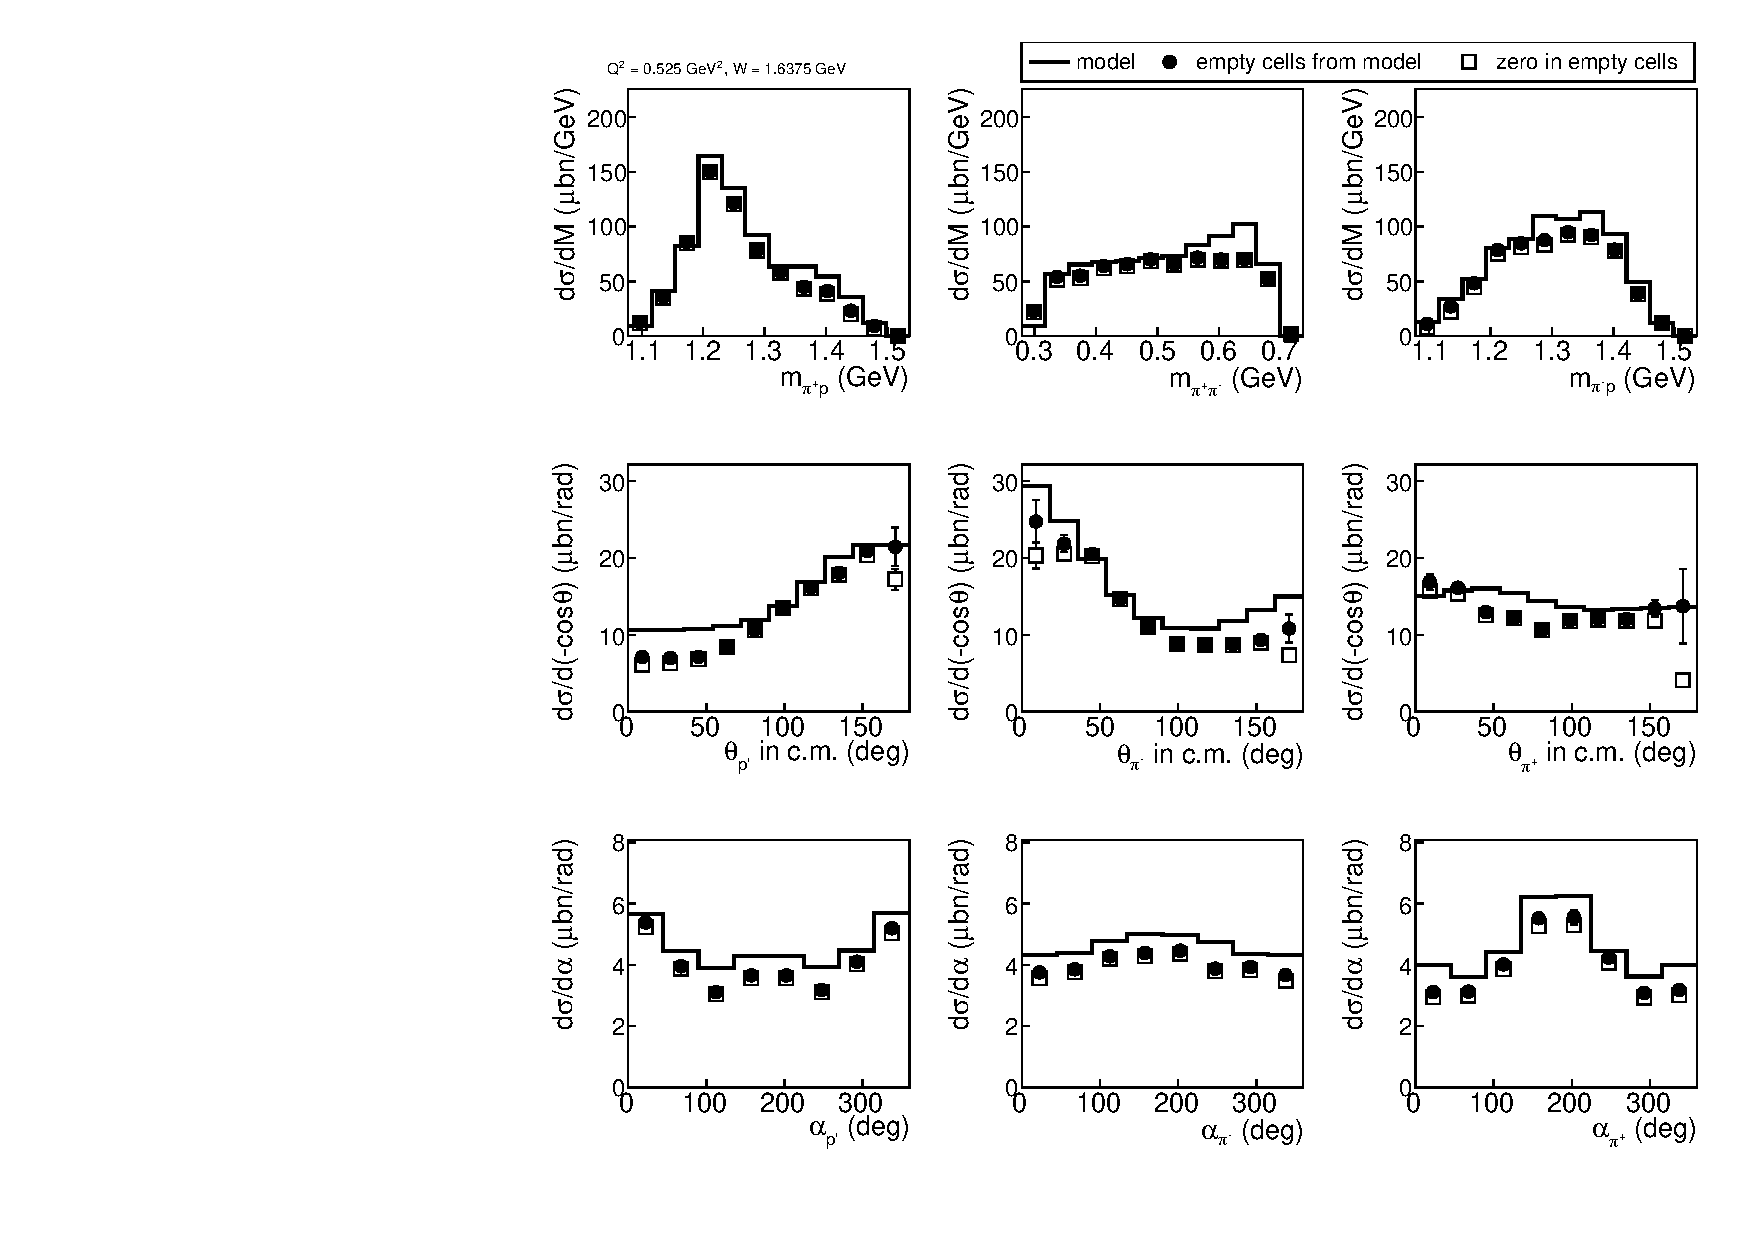
\includegraphics[width=13cm,keepaspectratio]{pictures/topologies/cr_sec_all_top.pdf}}
\caption{\small  
The extracted single-differential cross sections  for the two cases: when the contribution from empty cells is ignored (empty squares) and when that is taken into account (black circles).
Curves show the TWOPEG cross sections that were used as a model assumption for the empty cell contribution. All distributions are given for one particular bin in $W$ and $Q^2$ ($W = 1.6375$~GeV, $Q^2 = 0.525$~GeV$^2$).} \label{fig:topologies}
\end{center}
\end{figure*}

%Include how empty cells were filled out + combinations of various topologies. 1D plots with comparison of the cross section with and without empty cells filled out. Describe efficiency error cut.

%It needs to be mentioned that kinematical cells where $N_{rec} >= N_{gen}$ are treated as empty cells with no efficiency. Such cells are very rare and usually located near the edges of the invariant mass distributions where the cross section is close to zero.




Due to the blind areas in the geometrical coverage of the CLAS detector, some kinematical bins of the double-pion production phase space turned out to have zero acceptance. 
In such bins, which are usually called empty cells,  the cross section can not be experimentally defined. The empty cells contribute to the integrals in~\eqref{inegr5diff} along with other kinematical bins.  Ignoring the contribution from empty cells leads to the systematical cross section underestimation and therefore some model assumtions for the cross section in these cells are needed. 

A special procedure was developed in order to take into account the contrubutions from empty cells to the integrals~\eqref{inegr5diff}.
As a first step of this procedure the map of the empty cells was determined using the Monte Carlo simulation. A cell is treated as empty, if it contains generated events ($N_{gen} > 0$), but does not contain any reconstructed events ($N_{rec} = 0$). 

Beside that, the efficiency in some kinematical bins can not be reliably determined due to the boundary effects, bin to bin event migration, and limited Monte Carlo statistics.  
These cells were excluded from the consideration and also treated as the empty cells.
In order to determine the criterion for cell exclusion the distribution shown in Fig.~\ref{fig:eff_err} is produced.
This figure shows the relative efficiency error $\frac{\delta F}{F}$ (absolute efficiency error $\delta F$ is defined in Sect.~\ref{stat_unc})  versus efficiency $F$, while the color code stands for the number of multi-dimensional cells. As it is seen in  Fig.~\ref{fig:eff_err} cells with relative efficiency errors greater than 30\% are clustered along the horizontal stripes. This effect  reveals the bins with small statistics of the generated events and originates from the fact that efficiency is obtained by division of two integer numbers. Moreover these horizontal stripes contain many non-trustable cells with extremely small efficiency. Therefore,  the multi-dimensional bins that are located above the horizontal  line in Fig.~\ref{fig:eff_err} are excluded from the analysis being treated as empty cells.



Once the map of empty cells had been determined the cross section produced by the TWOPEG event  generator was used as a model assumption for these kinematical bins. 
This event generator employs the double-pion cross sections from the recent version of the JM15 model fit to the data~\cite{Ripani:2002ss,Mokeev:2012vsa,Fedotov:2008aa,Golovach:note}) as well as the data~\cite{Wu:2005wf,ABBHHM:1968aa} itself and therefore provides the best cross section estimation up to now.
The paper~\cite{Skorodum:EG} describes in details the approach used in TWOPEG in order to estimate the cross section value. 



Fig.~\ref{fig:topologies} introduces the single-differential cross sections given by Eq.~\eqref{inegr5diff} extracted for three sets of the kinematical variables described in Sect.~\ref{sec_kin_var}.  The empty squares correspond to the case, when the contribution from empty cells is ignored, the  black circles are for the case, when that is taken into account in the way described above, while the black curves stand for the TWOPEG cross sections which were used as a model assumtion. The figure demonstrates reasonably small contribution from empty cells that was achieved using all four avaliable reaction topologies in combination. Only the edge points in $\theta$ distributions reveal pronounceable empty cell contributions  due to the complete absence of the CLAS acceptance in the corresponding directions. 
To account for the possible descrepancies with the model, the part of the cross section that comes from the empty cells was assigned with 50\% relative error. Finally this additional error was combined with the total statistical one. 






\subsection{Radiative correction}
\label{rad_corr}


The radiative correction to the extracted cross sections was performed using TWOPEG event generator for the double-pion electroproduction~\cite{Skorodum:EG} which accounts the radiative effects by means of the well-known approach~\cite{Mo:1968cg}. 
This approach has successfully proven itself as an efficient tool to calculate inclusive radiative cross section from the non-radiative one.
In~\cite{Mo:1968cg} the approach is applied to the inclusive case, while in TWOPEG double pion integral cross sections are used instead~\cite{Skorodum:EG}. The radiative photons are suposed to be emitted colliniarly either to the direction of the initial or scattered electron (so-called ``peaking approximation").

In~\cite{Mo:1968cg,Skorodum:EG} the calculation of the radiative cross section is split into two parts. The ``soft" part assumes the energy of the  emitted radiative photon to be less than the certain minimal value (10 MeV), while the ``hard" part is for the photons with energy greater than that value. 
The ``soft" part is evaluated
explicitly, while for the calculation of the ``hard" part the inclusive hadronic
tensor is assumed. 
The latter assumption is however considered adequate, since the approaches
that are capable at describing radiative processes
in exclusive double-pion electroproduction, are not yet available.

\begin{figure}[htp]
\begin{center}
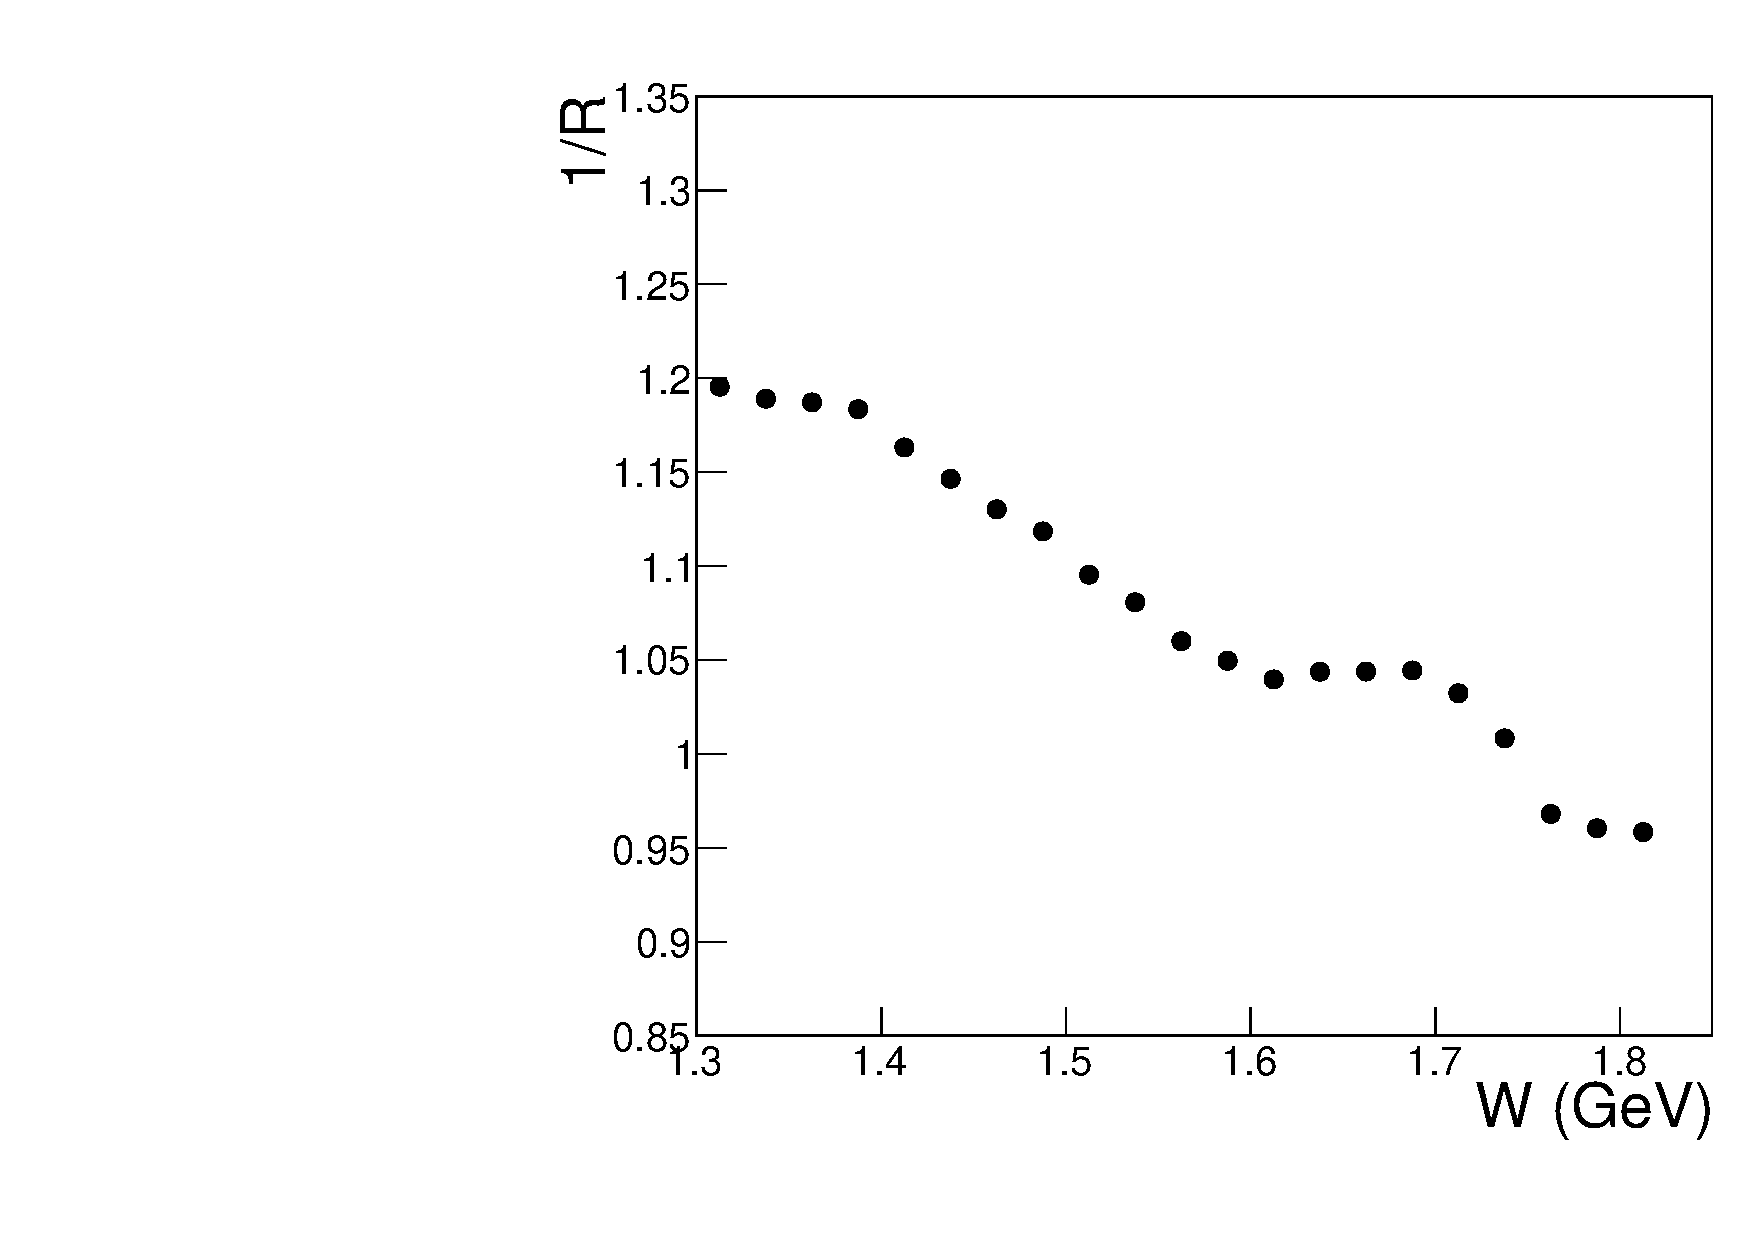
\includegraphics[width=8cm]{pictures/rad_corr/rad_corr_avrg.pdf}
\caption{\small One over radiative correction factor $R$ (see Eq.~\ref{expcrossect})
as function of $W$ averaged over all considered $Q^{2}$ bins.} \label{radcorrfact}
\end{center}
\end{figure}


The radiative
correction factor $R$ in Eq.~(\ref{expcrossect})
was determined in the following way.
The double-pion events either with and without radiative effects were generated with TWOPEG, then the ratio given by Eq.~\eqref{radcorrfact} was taken in each $\Delta W \Delta Q^{2}$ bin. 
\begin{equation}
\label{radcorrfact}
R(\Delta W,\Delta Q^{2}) = \frac{N_{rad}^{2D}}{N_{norad}^{2D}} \textrm{ ,}
\end{equation}
where $N_{rad}^{2D}$ and $N_{norad}^{2D}$ are the
numbers of generated events in each $\Delta W \Delta Q^{2}$ bin
with and without radiative effects, respectively.



The used approach allows to obtain the correction factor $R$ only as a function of $W$ and $Q^{2}$ disregarding its dependence on the final hadron variables.
However 
the need to integrate the cross section at least over four final hadron variables (see Eq.~\eqref{inegr5diff}) considerably reduces the influence of
the final hadron kinematics on the
radiative correction factor thus even stronger justifying 
the applicability of the procedure~\cite{Mo:1968cg,Skorodum:EG}.




 The quantity one over $R$, which is averaged over all considered $Q^{2}$ bins, is plotted in  Fig.~\ref{radcorrfact} as a function of $W$. The dependence of this quantity on $Q^{2}$ was found to be negligible.  The uncertainties associated with the statistics of the generated events are very small and therefore  not seen in Fig.~\ref{radcorrfact}.















\subsection{Statistical uncertainties}
\label{stat_unc}

The limited statistics of either the experimental data and the Monte Carlo simulation  are two sources of the statistical fluctuations of the extracted cross sections.
The cut on the efficiency error discribed in Sec.~\ref{eff_err} is chosen in a way that the latter source gives the minor contribution to the total statistical uncertainty .


The absolute statistical  uncertainty to the five-differential
virtual photoproduction cross section caused by the statistics of the experimental data can be written as
 \begin{equation}
\delta_{stat,exp}(\Delta^{5} \tau) = \frac{1}{F} \frac{1}{R}
\frac{1}{ \Gamma_{v} }
\frac{\sqrt{\left( \frac{\Delta
N_{full}}{Q_{full}^{2}}+\frac{\Delta N_{empty}}{Q_{empty}^{2}} \right) } }{
\Delta W \Delta Q^{2} \Delta^{5} \tau \left( \frac{l \rho N_{A}}{q_{e}M_{H}} \right)}.
\label{staterrors}
\end{equation}


The absolute error to the cross section due to the limited Monte Carlo statistic is  in turn given by
\begin{equation}
\delta_{stat,MC} = \frac{d^{5}\sigma}{d^{5}\tau} \left( \frac{\delta F)}{F} \right),
\label{montecarloerror}
\end{equation}

where $F$ is the efficiency inside the multi-dimetional bin defined by Eq.~\eqref{efficiency}, while $\delta F$ is its absolute statistical error. 



Due to the fact that $N_{gen}$ and $N_{rec}$ in Eq.~\eqref{efficiency} are not independent the usual method of partial dirivatives is not applicable in order to calculate $\delta F$.
Therefore the special approach described in~\cite{Laforge:1996ts} was used for this purpose.
Neglecting the event migration between the bins, this approach gives the following expression for  
 the absolute statistical error of the efficiency
\begin{equation}
\delta F =
\sqrt{\frac{(N_{gen}-N_{rec})N_{rec}}{N_{gen}^{3}}}.
\label{efferror}
\end{equation}

Finally two parts of the statistical uncertainty given by Eq.~\eqref{staterrors} and \eqref{montecarloerror} are combined quadratically into the total absolute statistical uncertainty to the cross section in the multi-demensional bin


\begin{equation}
\delta_{stat,tot} =
\sqrt{\delta_{stat,exp}^{2} + \delta_{stat,MC}^{2}}.
\label{errortot}
\end{equation}











\subsection{Systematical uncertainties}

The systematical uncertainties in this experiment appear to dominate the statistical ones and originate from the several sources.

The presence of the elastic events
in the dataset advantages the normalization verification of the extracted cross sections. For this purpose the elastic cross section was extracted and compared with the parametrization~\cite{Bosted:1994tm}, and 3\% fluctuation was revealed. Therefore this value was included into the systematical uncertainty  to the extracted double-pion cross sections as a global factor. This factor takes into account  inaccuracy in the luminosity calculation (due to miscalibrations of the Faraday cup, target
density instabilities, etc.) as well as errors in the electron registration and identification.


In order to study the systematical uncertainties, the double pion cross sections were obtained using the alternative method of the topology combination. In contrast with the main method, where the events from all four topologies were summed up in each multidumention bin, the alternative one considered only the events from the topology with the maximal efficiency. 
 The difference between the cross sections obtained in these two ways was interpreted as a systematical uncertainty.
Since various topologies correspond to the different registered final hadrons  this uncertainty includes the errors due to the hadron registration and identification. 
This uncertainty was calculated for each bin in  $W$ and $Q^{2}$ and found to be of the order of 2\%.




According to Sect.~\ref{sec_kin_var} the double-pion cross sections was extracted in three sets of the  kinematical variables. The difference between the cross sections obtained by integration over these three kinematical grids was interpreted as a systematical uncertainty. This  uncertainty was computed for each bin in $W$ and $Q^{2}$ and was typically of the order of 5\%.
As the final results, the integrated cross sections that were averaged over these three grids are reported.


Beside that, as a common practice~\cite{Fedotov:2008aa,Isupov:2017lnd},  an extra 5\% global uncertainty was assigned to the cross section due to the inclusive radiative correction procedure (see Sect.~\ref{rad_corr}).


The uncertainties due to the sources mentioned above were summed up in qudrature to obtain the total systematical uncertainty to the integral double pion cross sections.



\section{Comparison with the model and previously avaliable data}

\subsection{Previously avaliable data}

\begin{figure*}[htp]
\begin{center}
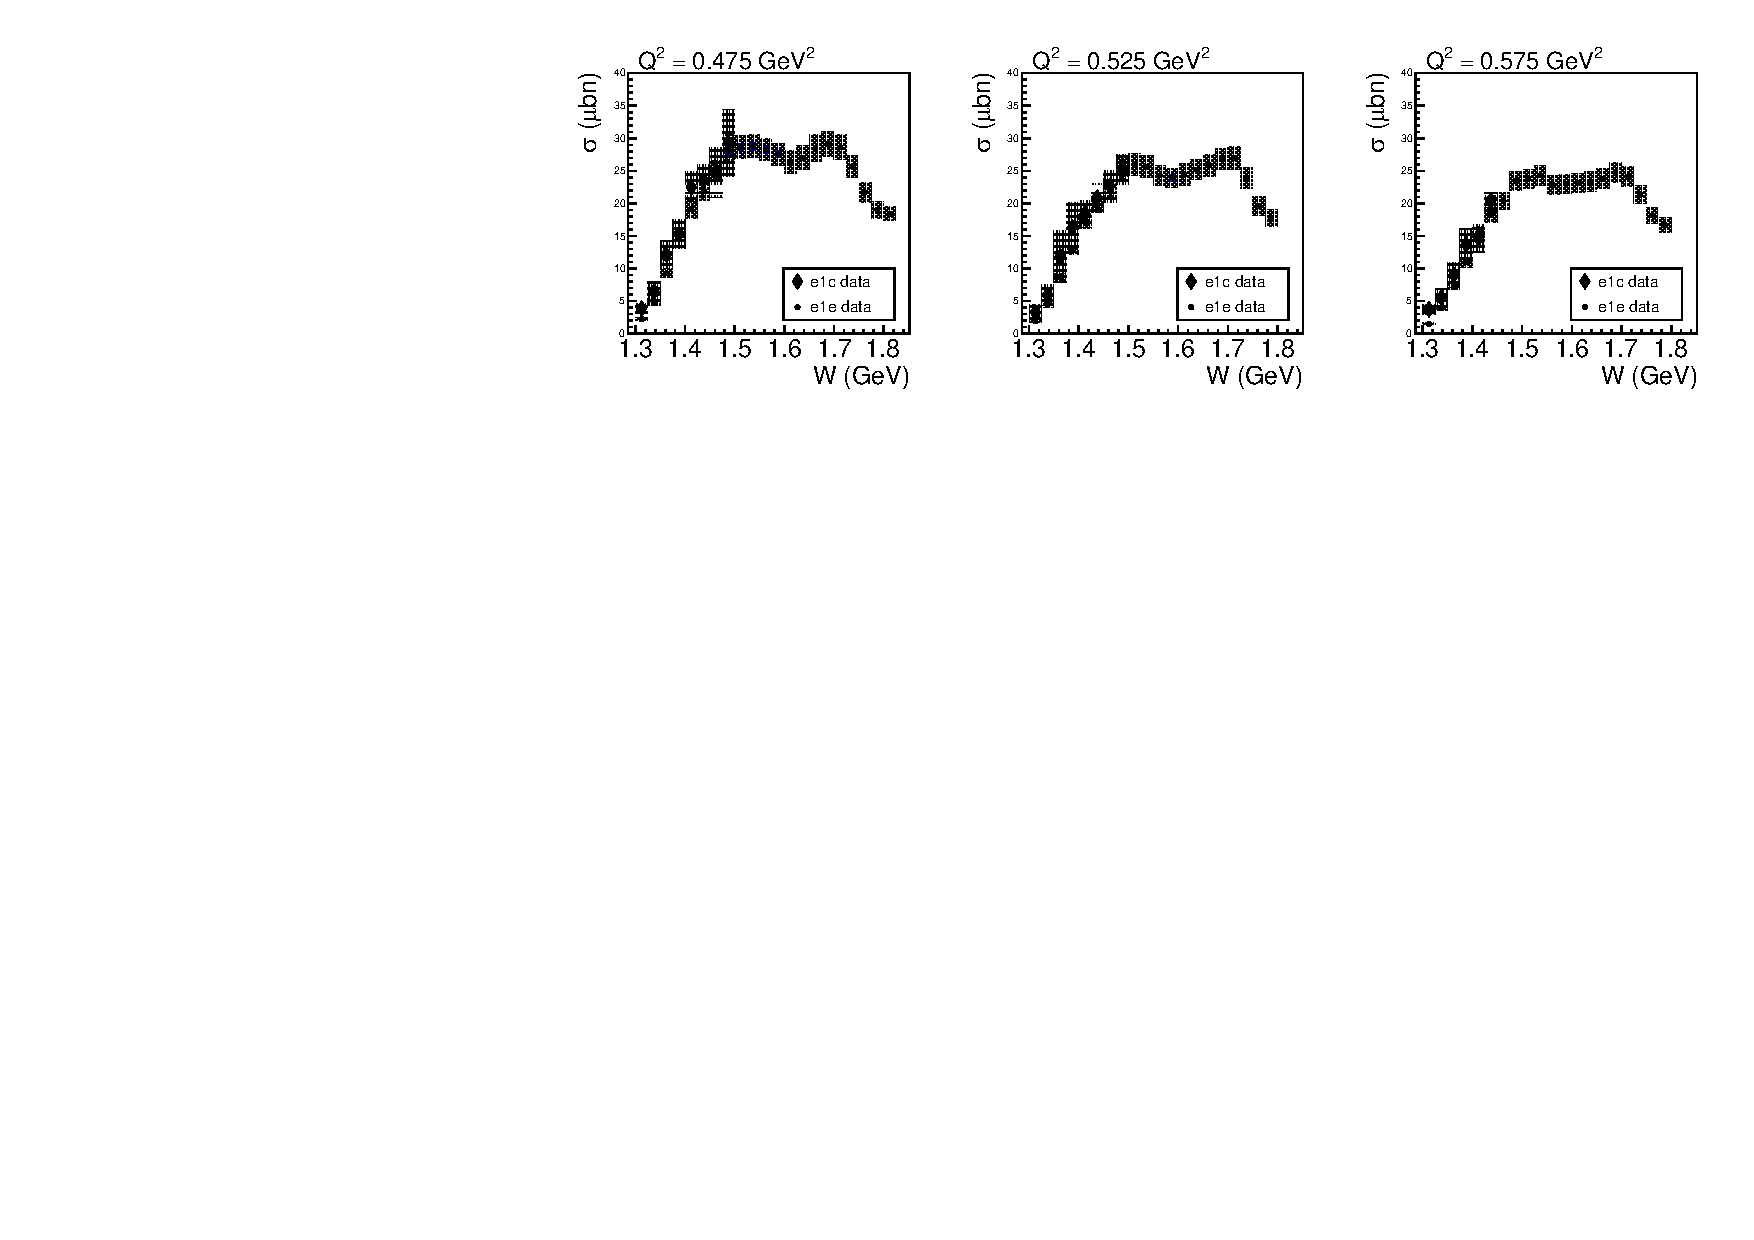
\includegraphics[width=15cm]{pictures/conclusions/e1e_e1c.pdf}
\caption{\small The $W$ dependencies of the extracted  cross sections (circles) in comparison with the avaliable data~\cite{Fedotov:2008aa} (dimonds) for three bins in $Q^{2}$. Hatched areas correspond to the total uncertainties (sistematical and statistical).}
\label{fig:e1e_e1c}
\end{center}
\end{figure*}


In Fig.~\ref{fig:e1e_e1c} the comparison of integral double pion cross sections with the avaliable data~\cite{Fedotov:2008aa} is shown. 
The cross sections~\cite{Fedotov:2008aa} were obtained with 1.515~GeV electron beam energy that makes their longitudinal parts slightly differ, thus intruducing a small systematical distortion into the comparison. The kinematical coverages of these two datasets overlap only in three bins in $Q^{2}$ which are shown in Fig.~\ref{fig:e1e_e1c}. Meanwhile, the cross sections presented here should be treated as more reliable since they were extracted with more advanced technique -- i.e., the combination of all four avaliable topologies was used instead of only two in the data~\cite{Fedotov:2008aa}, the map of empty cells was better determined using  the cut on the efficiency error, the contribution from the empty cells was accounted for by the advanced method using TWOPEG~\cite{Skorodum:EG}, and furthermore, finer binning in hadron variables was achieved. Nevertheless, Fig.~\ref{fig:e1e_e1c} demonstrates reasonable agreement between these two sets of cross sections within the total uncertainties.  


\subsection{Comparison with the model }

\begin{figure*}[htp]
\begin{center}
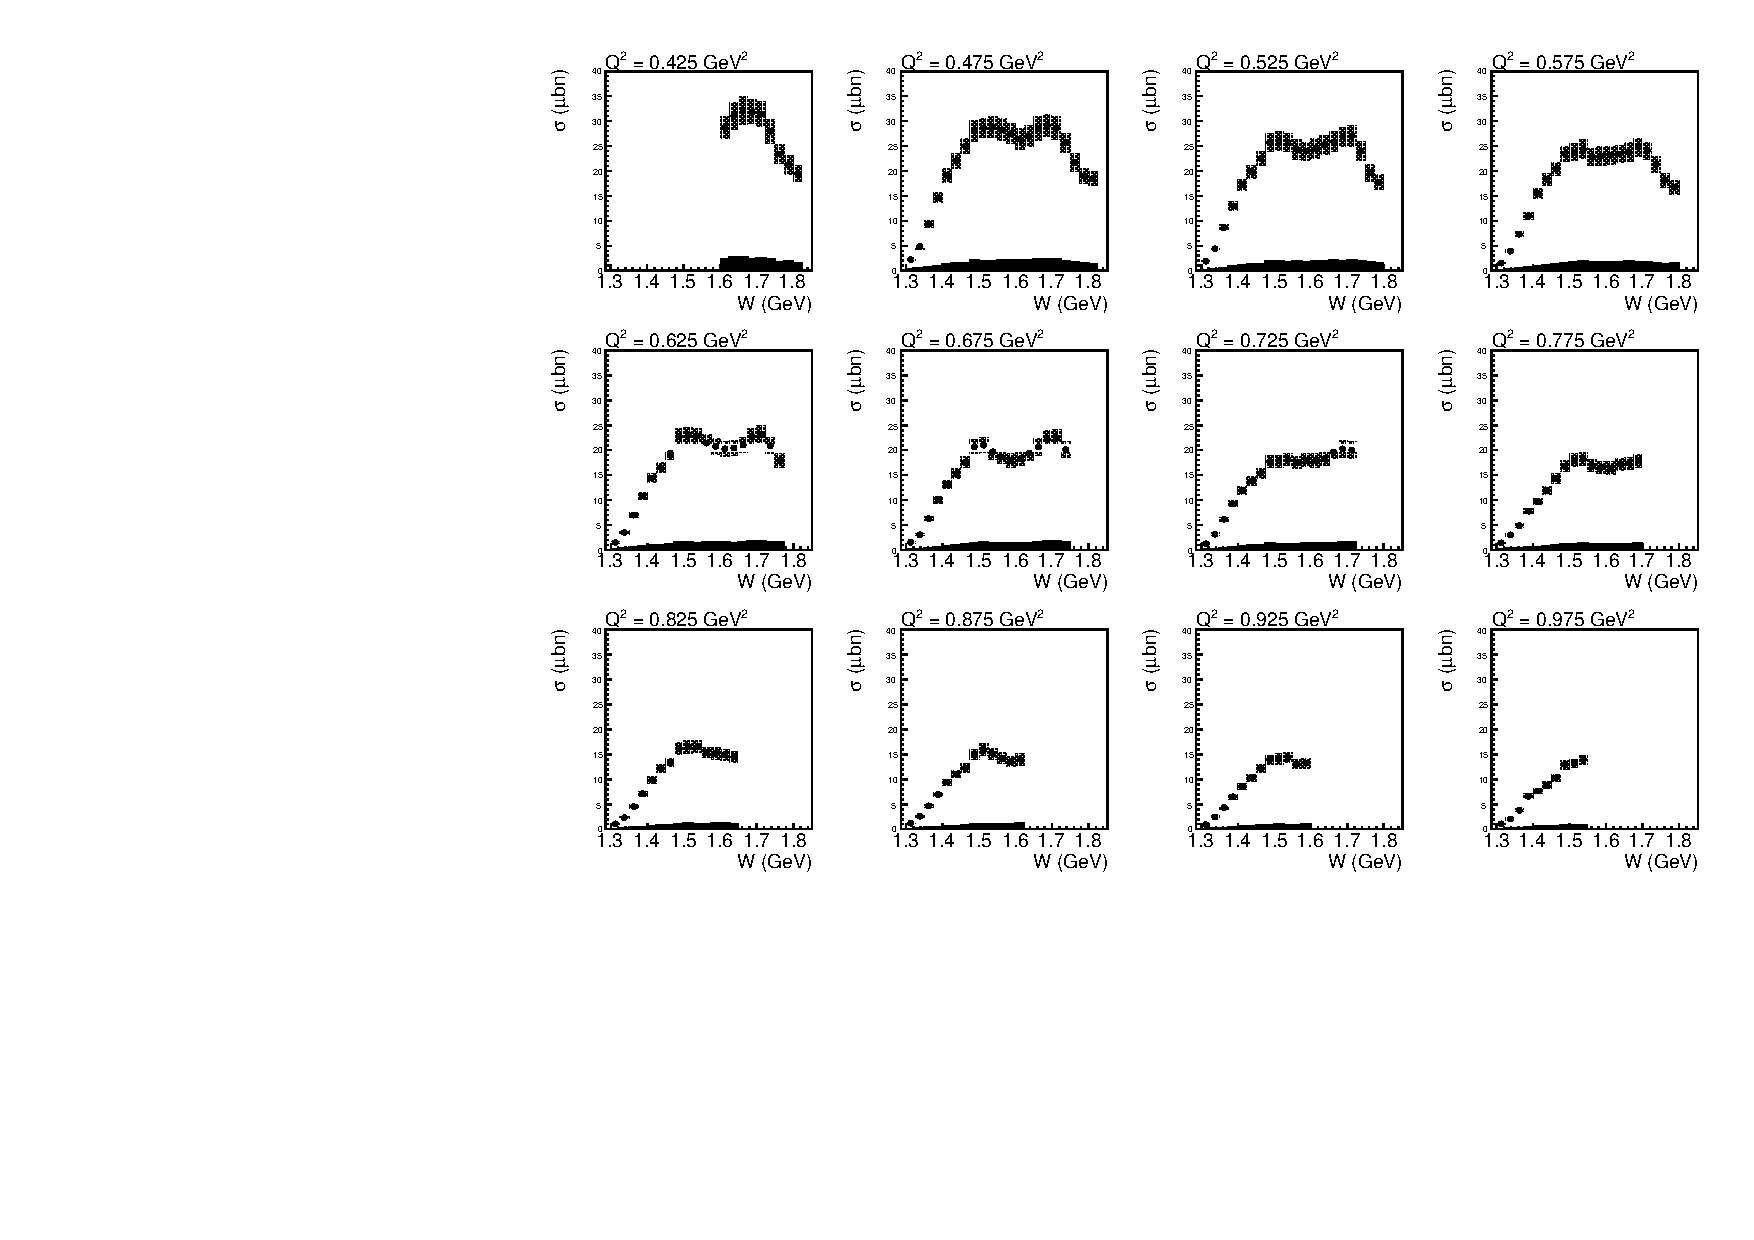
\includegraphics[width=15cm]{pictures/sys_err/sys_err.pdf}
\caption{\small Systematical errors of the integrated cross sections. The plots show $W$ dependencies of the integrated cross section in various bins in $Q^{2}$. The systematical uncertanties are shown as the black bands at the bottom of each plot. The total cross section uncertainty (both statistical and systematical ones summed up in quadrature) is shown by the hatched black areas.}
\label{fig:sys_err}

\end{center}
\end{figure*}



1D plot for one Q2 \& W bin + int plots with sys errors.

\section{CONCLUSIONS}





Comparison with previously avaliable data.

\begin{acknowledgments}


\end{acknowledgments}

\clearpage
\section*{Appendix A: The definition of the angle $\alpha$}
\label{app_a}


The calculation of the angle $\alpha_{\pi^{-}}$ from the second set of hadron variables mentioned in Sec.~\ref{sec_kin_var} is given below. The angles $\alpha_{p'}$ and $\alpha_{\pi^{+}}$ from two other sets are calculated analogously~\cite{Fed_an_note:2017}.

The angle $\alpha_{\pi^{-}}$ is the angle between two planes A and B (see Fig.~\ref{fig:cr_sec_kinematic2}).
The plane A is defined by
the initial proton and $\pi^{-}$, while the plane B is defined by the momenta of
all final hadrons. Note that the three-momenta of $\pi^{+}$,
$\pi^{-}$, $p'$ are in the same plane, since in c.m.s.
their total three-momentum has to be equal to zero.


\begin{figure}[htp]
\begin{center}
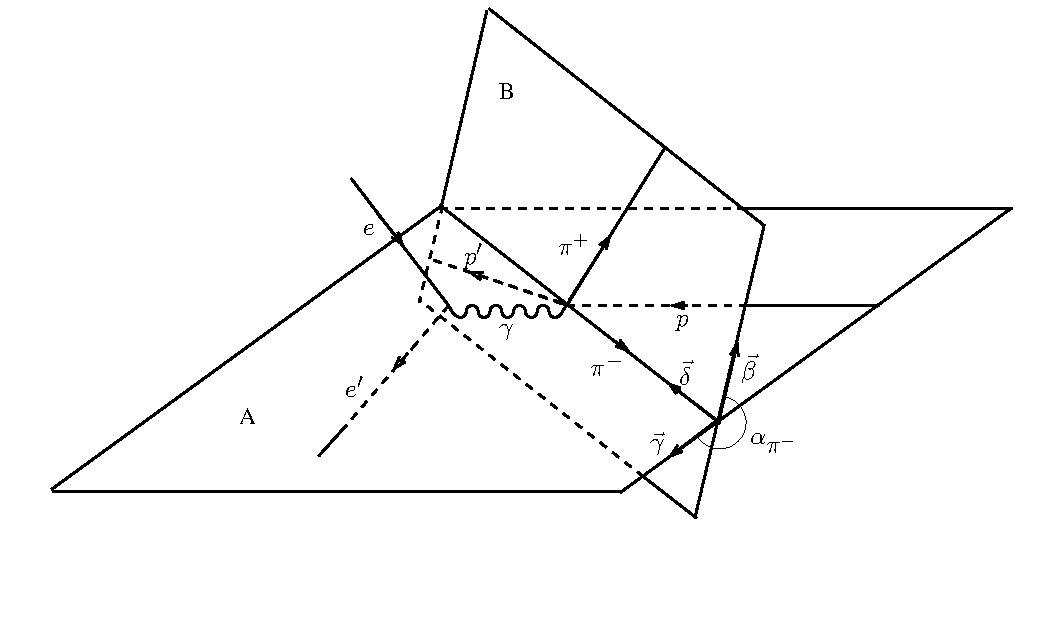
\includegraphics[width=8cm]{pictures/angles/alpha1.pdf}
\caption{\small Definition of the angle $\alpha_{\pi^{-}}$ between two planes: the plane B is defined by the three-momenta of all final hadrons, while the plane A defined by  the three-momenta of $\pi^{-}$ and initial proton. The definitions of  auxiliary vectors $\vec \beta$, $\vec \gamma$, $\vec \delta$ are given in the text.} \label{fig:cr_sec_kinematic2}
\end{center}
\end{figure}


To calculate the angle $\alpha_{\pi^{-}}$ firstly two
auxiliary vectors $\vec \gamma$  and
$\vec \beta$ should be determined. The vector $\vec \gamma$ is the unit vector perpendicular to the three-momentum
$\vec P_{\pi^{-}}$, directed toward the vector $(-\vec n_{z})$ and situated in the plane A. $\vec
n_{z}$ is the unit vector directed along $z$-axis.
The vector $\vec \beta$ is the unit vector perpendicular to the three-momentum of $\pi^{-}$, 
directed toward the three-momentum of $\pi^{+}$ and situated in the plane B. 
 Then the angle between two planes  $\alpha_{\pi^{-}}$ is
\begin{equation}
\alpha_{\pi^{-}} = acos(\vec \gamma \cdot \vec \beta),
\label{eq:cr_sec_anglealpha}
\end{equation}
where $acos$ is a function that runs between zero and
$\pi$, while the angle $\alpha_{\pi^{-}}$ may vary between zero and
$2\pi$. To determine the $\alpha$ angle in the
range between $\pi$ and $2\pi$ 
the relative direction between the $\pi^{-}$ three-momentum and the vector product $\vec \delta = [ \vec \gamma \times \vec \beta ]$ of the auxiliary vectors $\vec
\gamma$ and $\vec \beta$ should be taken into account.
%\begin{equation}
%\vec \delta = [ \vec \gamma \times \vec \beta ]
%\label{vecprod}
%\end{equation}
If the vector $\vec \delta$ is colinear to the three-momentum of $\pi^{-}$, the angle $\alpha_{\pi^{-}}$ is determined
by~(\ref{eq:cr_sec_anglealpha}), and in a case of anti-collinearity by
\begin{equation}
\alpha_{\pi^{-}} = 2\pi - acos(\vec \gamma \cdot \vec \beta).
\label{eq:cr_sec_anglealpha_var}
\end{equation}
The defined above vector $\vec \gamma$ can be expressed as
\begin{eqnarray}
\vec \gamma = a_{\alpha}(-\vec n_{z}) + b_{\alpha}\vec n_{P_{\pi^{-}}} & \text{with} \nonumber \\
a_{\alpha} = \sqrt{\frac{1}{1 - (\vec n_{P_{\pi^{-}}} \cdot (-\vec n_{z} ) )^{2}}} & \text{and} \label{alphavec}\\
b_{\alpha} = - (\vec n_{P_{\pi^{-}}} \cdot (-\vec n_{z} ) ) a_{\alpha} \textrm{ ,} \nonumber
\end{eqnarray} 
where $\vec n_{P_{\pi^{-}}}$ is the unit vector directed along the three-momentum of $\pi^{-}$ (see Fig.~\ref{fig:cr_sec_kinematic2}).

Taking the scalar products $(\vec \gamma \cdot \vec
n_{P_{\pi^{-}}})$ and $(\vec \gamma \cdot \vec  \gamma)$,
it is straightforward to verify, that $\vec \gamma$ is the unit vector perpendicular to the three-momentum of $\pi^{-}$.

The vector $\vec \beta$ can be obtained as
\begin{eqnarray}
\vec \beta = a_{\beta}\vec n_{P_{\pi^{+}}} + b_{\beta}\vec n_{P_{\pi^{-}}} & \text{with} \nonumber \\
a_{\beta} = \sqrt{\frac{1}{1 - (\vec n_{P_{\pi^{+}}} \cdot \vec n_{P_{\pi^{-}}})^{2}}} & \text{and} \label{betavec}\\
b_{\beta} = - (\vec n_{P_{\pi^{+}}} \cdot \vec n_{P_{\pi^{-}}}) a_{\beta} \textrm{ ,} \nonumber
\end{eqnarray} 
where $\vec n_{P_{\pi^{+}}}$ is the unit vector directed along the three-momentum of $\pi^{+}$.

Again taking the scalar products $(\vec \beta \cdot \vec
n_{P_{\pi^{-}}})$ and $(\vec \beta \cdot \vec  \beta)$,
it is straightforward to see, that $\vec \beta$ is
the unit vector perpendicular to the 
three-momentum of $\pi^{-}$. 






Further detailed information about kinematic of the reactions with three-particle final states can be found here~\cite{Byckling:1971vca}.



\bibliography{e1e_paper}{}
\bibliographystyle{apsrev4-1}
%\include{appendix1}


\end{document}
